\documentclass[twoside]{book}

% Packages required by doxygen
\usepackage{calc}
\usepackage{doxygen}
\usepackage{graphicx}
\usepackage[utf8]{inputenc}
\usepackage{makeidx}
\usepackage{multicol}
\usepackage{multirow}
\usepackage{textcomp}
\usepackage[table]{xcolor}

% Font selection
\usepackage[T1]{fontenc}
\usepackage{mathptmx}
\usepackage[scaled=.90]{helvet}
\usepackage{courier}
\usepackage{amssymb}
\usepackage{sectsty}
\renewcommand{\familydefault}{\sfdefault}
\allsectionsfont{%
  \fontseries{bc}\selectfont%
  \color{darkgray}%
}
\renewcommand{\DoxyLabelFont}{%
  \fontseries{bc}\selectfont%
  \color{darkgray}%
}

% Page & text layout
\usepackage{geometry}
\geometry{%
  a4paper,%
  top=2.5cm,%
  bottom=2.5cm,%
  left=2.5cm,%
  right=2.5cm%
}
\tolerance=750
\hfuzz=15pt
\hbadness=750
\setlength{\emergencystretch}{15pt}
\setlength{\parindent}{0cm}
\setlength{\parskip}{0.2cm}
\makeatletter
\renewcommand{\paragraph}{%
  \@startsection{paragraph}{4}{0ex}{-1.0ex}{1.0ex}{%
    \normalfont\normalsize\bfseries\SS@parafont%
  }%
}
\renewcommand{\subparagraph}{%
  \@startsection{subparagraph}{5}{0ex}{-1.0ex}{1.0ex}{%
    \normalfont\normalsize\bfseries\SS@subparafont%
  }%
}
\makeatother

% Headers & footers
\usepackage{fancyhdr}
\pagestyle{fancyplain}
\fancyhead[LE]{\fancyplain{}{\bfseries\thepage}}
\fancyhead[CE]{\fancyplain{}{}}
\fancyhead[RE]{\fancyplain{}{\bfseries\leftmark}}
\fancyhead[LO]{\fancyplain{}{\bfseries\rightmark}}
\fancyhead[CO]{\fancyplain{}{}}
\fancyhead[RO]{\fancyplain{}{\bfseries\thepage}}
\fancyfoot[LE]{\fancyplain{}{}}
\fancyfoot[CE]{\fancyplain{}{}}
\fancyfoot[RE]{\fancyplain{}{\bfseries\scriptsize Generated on Wed Jun 5 2013 23:45:49 for oFreq by Doxygen }}
\fancyfoot[LO]{\fancyplain{}{\bfseries\scriptsize Generated on Wed Jun 5 2013 23:45:49 for oFreq by Doxygen }}
\fancyfoot[CO]{\fancyplain{}{}}
\fancyfoot[RO]{\fancyplain{}{}}
\renewcommand{\footrulewidth}{0.4pt}
\renewcommand{\chaptermark}[1]{%
  \markboth{#1}{}%
}
\renewcommand{\sectionmark}[1]{%
  \markright{\thesection\ #1}%
}

% Indices & bibliography
\usepackage{natbib}
\usepackage[titles]{tocloft}
\setcounter{tocdepth}{3}
\setcounter{secnumdepth}{5}
\makeindex

% Hyperlinks (required, but should be loaded last)
\usepackage{ifpdf}
\ifpdf
  \usepackage[pdftex,pagebackref=true]{hyperref}
\else
  \usepackage[ps2pdf,pagebackref=true]{hyperref}
\fi
\hypersetup{%
  colorlinks=true,%
  linkcolor=blue,%
  citecolor=blue,%
  unicode%
}

% Custom commands
\newcommand{\clearemptydoublepage}{%
  \newpage{\pagestyle{empty}\cleardoublepage}%
}


%===== C O N T E N T S =====

\begin{document}

% Titlepage & ToC
\hypersetup{pageanchor=false}
\pagenumbering{roman}
\begin{titlepage}
\vspace*{7cm}
\begin{center}%
{\Large o\-Freq \\[1ex]\large 1.\-0 }\\
\vspace*{1cm}
{\large Generated by Doxygen 1.8.4}\\
\vspace*{0.5cm}
{\small Wed Jun 5 2013 23:45:49}\\
\end{center}
\end{titlepage}
\clearemptydoublepage
\tableofcontents
\clearemptydoublepage
\pagenumbering{arabic}
\hypersetup{pageanchor=true}

%--- Begin generated contents ---
\chapter{Hierarchical Index}
\section{Class Hierarchy}
This inheritance list is sorted roughly, but not completely, alphabetically\-:\begin{DoxyCompactList}
\item \contentsline{section}{Active\-Force\-Matrix}{\pageref{class_active_force_matrix}}{}
\item \contentsline{section}{Body}{\pageref{class_body}}{}
\item \contentsline{section}{Body\-With\-Force\-Matrix}{\pageref{class_body_with_force_matrix}}{}
\item \contentsline{section}{Body\-With\-Solution}{\pageref{class_body_with_solution}}{}
\item \contentsline{section}{Derivative}{\pageref{class_derivative}}{}
\item \contentsline{section}{Equation}{\pageref{class_equation}}{}
\item \contentsline{section}{Equation\-Of\-Motion}{\pageref{class_equation_of_motion}}{}
\begin{DoxyCompactList}
\item \contentsline{section}{Equation\-Of\-Motion\-\_\-01}{\pageref{class_equation_of_motion__01}}{}
\end{DoxyCompactList}
\item \contentsline{section}{File\-Writer}{\pageref{class_file_writer}}{}
\item \contentsline{section}{Force}{\pageref{class_force}}{}
\begin{DoxyCompactList}
\item \contentsline{section}{Force\-Active}{\pageref{class_force_active}}{}
\item \contentsline{section}{Force\-Reactive}{\pageref{class_force_reactive}}{}
\begin{DoxyCompactList}
\item \contentsline{section}{Force\-Cross\-Body}{\pageref{class_force_cross_body}}{}
\end{DoxyCompactList}
\end{DoxyCompactList}
\item \contentsline{section}{Motion\-Model}{\pageref{class_motion_model}}{}
\item \contentsline{section}{Motion\-Solver}{\pageref{class_motion_solver}}{}
\item \contentsline{section}{Output\-Derived}{\pageref{class_output_derived}}{}
\begin{DoxyCompactList}
\item \contentsline{section}{Global\-Solution}{\pageref{class_global_solution}}{}
\begin{DoxyCompactList}
\item \contentsline{section}{Global\-Acceleration}{\pageref{class_global_acceleration}}{}
\item \contentsline{section}{Global\-Motion}{\pageref{class_global_motion}}{}
\item \contentsline{section}{Global\-Velocity}{\pageref{class_global_velocity}}{}
\end{DoxyCompactList}
\end{DoxyCompactList}
\item \contentsline{section}{Outputs\-Body}{\pageref{class_outputs_body}}{}
\item \contentsline{section}{Outputs\-List}{\pageref{class_outputs_list}}{}
\item \contentsline{section}{Reactive\-Force\-Matrix}{\pageref{class_reactive_force_matrix}}{}
\item \contentsline{section}{Read\-Input}{\pageref{class_read_input}}{}
\begin{DoxyCompactList}
\item \contentsline{section}{Bodiesinput}{\pageref{class_bodiesinput}}{}
\item \contentsline{section}{Control\-Input}{\pageref{class_control_input}}{}
\item \contentsline{section}{Data\-Input}{\pageref{class_data_input}}{}
\item \contentsline{section}{Forces\-Input}{\pageref{class_forces_input}}{}
\item \contentsline{section}{Hydrodynamic\-Input}{\pageref{class_hydrodynamic_input}}{}
\item \contentsline{section}{Seaenv\-Input}{\pageref{class_seaenv_input}}{}
\end{DoxyCompactList}
\item \contentsline{section}{Sea\-Enviroment}{\pageref{class_sea_enviroment}}{}
\item \contentsline{section}{System}{\pageref{class_system}}{}
\item \contentsline{section}{User\-Forces}{\pageref{class_user_forces}}{}
\item \contentsline{section}{Wave\-Directions}{\pageref{class_wave_directions}}{}
\item \contentsline{section}{Wave\-Frequencies}{\pageref{class_wave_frequencies}}{}
\item \contentsline{section}{Wave\-Spectrum\-Model}{\pageref{class_wave_spectrum_model}}{}
\item \contentsline{section}{Wave\-Spread\-Model}{\pageref{class_wave_spread_model}}{}
\end{DoxyCompactList}

\chapter{Class Index}
\section{Class List}
Here are the classes, structs, unions and interfaces with brief descriptions\-:\begin{DoxyCompactList}
\item\contentsline{section}{\hyperlink{class_active_force_matrix}{Active\-Force\-Matrix} }{\pageref{class_active_force_matrix}}{}
\item\contentsline{section}{\hyperlink{class_bodiesinput}{Bodiesinput} }{\pageref{class_bodiesinput}}{}
\item\contentsline{section}{\hyperlink{class_body}{Body} }{\pageref{class_body}}{}
\item\contentsline{section}{\hyperlink{class_body_with_force_matrix}{Body\-With\-Force\-Matrix} }{\pageref{class_body_with_force_matrix}}{}
\item\contentsline{section}{\hyperlink{class_body_with_solution}{Body\-With\-Solution} }{\pageref{class_body_with_solution}}{}
\item\contentsline{section}{\hyperlink{class_control_input}{Control\-Input} }{\pageref{class_control_input}}{}
\item\contentsline{section}{\hyperlink{class_data_input}{Data\-Input} }{\pageref{class_data_input}}{}
\item\contentsline{section}{\hyperlink{class_derivative}{Derivative} }{\pageref{class_derivative}}{}
\item\contentsline{section}{\hyperlink{class_equation}{Equation} }{\pageref{class_equation}}{}
\item\contentsline{section}{\hyperlink{class_equation_of_motion}{Equation\-Of\-Motion} }{\pageref{class_equation_of_motion}}{}
\item\contentsline{section}{\hyperlink{class_equation_of_motion__01}{Equation\-Of\-Motion\-\_\-01} }{\pageref{class_equation_of_motion__01}}{}
\item\contentsline{section}{\hyperlink{class_file_writer}{File\-Writer} }{\pageref{class_file_writer}}{}
\item\contentsline{section}{\hyperlink{class_force}{Force} }{\pageref{class_force}}{}
\item\contentsline{section}{\hyperlink{class_force_active}{Force\-Active} }{\pageref{class_force_active}}{}
\item\contentsline{section}{\hyperlink{class_force_cross_body}{Force\-Cross\-Body} }{\pageref{class_force_cross_body}}{}
\item\contentsline{section}{\hyperlink{class_force_reactive}{Force\-Reactive} }{\pageref{class_force_reactive}}{}
\item\contentsline{section}{\hyperlink{class_forces_input}{Forces\-Input} }{\pageref{class_forces_input}}{}
\item\contentsline{section}{\hyperlink{class_global_acceleration}{Global\-Acceleration} }{\pageref{class_global_acceleration}}{}
\item\contentsline{section}{\hyperlink{class_global_motion}{Global\-Motion} }{\pageref{class_global_motion}}{}
\item\contentsline{section}{\hyperlink{class_global_solution}{Global\-Solution} }{\pageref{class_global_solution}}{}
\item\contentsline{section}{\hyperlink{class_global_velocity}{Global\-Velocity} }{\pageref{class_global_velocity}}{}
\item\contentsline{section}{\hyperlink{class_hydrodynamic_input}{Hydrodynamic\-Input} }{\pageref{class_hydrodynamic_input}}{}
\item\contentsline{section}{\hyperlink{class_motion_model}{Motion\-Model} }{\pageref{class_motion_model}}{}
\item\contentsline{section}{\hyperlink{class_motion_solver}{Motion\-Solver} }{\pageref{class_motion_solver}}{}
\item\contentsline{section}{\hyperlink{class_output_derived}{Output\-Derived} }{\pageref{class_output_derived}}{}
\item\contentsline{section}{\hyperlink{class_outputs_body}{Outputs\-Body} }{\pageref{class_outputs_body}}{}
\item\contentsline{section}{\hyperlink{class_outputs_list}{Outputs\-List} }{\pageref{class_outputs_list}}{}
\item\contentsline{section}{\hyperlink{class_reactive_force_matrix}{Reactive\-Force\-Matrix} }{\pageref{class_reactive_force_matrix}}{}
\item\contentsline{section}{\hyperlink{class_read_input}{Read\-Input} }{\pageref{class_read_input}}{}
\item\contentsline{section}{\hyperlink{class_seaenv_input}{Seaenv\-Input} }{\pageref{class_seaenv_input}}{}
\item\contentsline{section}{\hyperlink{class_sea_enviroment}{Sea\-Enviroment} }{\pageref{class_sea_enviroment}}{}
\item\contentsline{section}{\hyperlink{class_system}{System} }{\pageref{class_system}}{}
\item\contentsline{section}{\hyperlink{class_user_forces}{User\-Forces} }{\pageref{class_user_forces}}{}
\item\contentsline{section}{\hyperlink{class_wave_directions}{Wave\-Directions} }{\pageref{class_wave_directions}}{}
\item\contentsline{section}{\hyperlink{class_wave_frequencies}{Wave\-Frequencies} }{\pageref{class_wave_frequencies}}{}
\item\contentsline{section}{\hyperlink{class_wave_spectrum_model}{Wave\-Spectrum\-Model} }{\pageref{class_wave_spectrum_model}}{}
\item\contentsline{section}{\hyperlink{class_wave_spread_model}{Wave\-Spread\-Model} }{\pageref{class_wave_spread_model}}{}
\end{DoxyCompactList}

\chapter{Class Documentation}
\hypertarget{class_active_force_matrix}{\section{Active\-Force\-Matrix Class Reference}
\label{class_active_force_matrix}\index{Active\-Force\-Matrix@{Active\-Force\-Matrix}}
}


{\ttfamily \#include $<$activeforcematrix.\-h$>$}

\subsection*{Public Member Functions}
\begin{DoxyCompactItemize}
\item 
\hyperlink{class_active_force_matrix_afb5b8d68549da5c8469b313fca84a5c9}{Active\-Force\-Matrix} ()
\item 
\hyperlink{class_active_force_matrix_a45a848d84e22a2503a4b111ccb571c9e}{$\sim$\-Active\-Force\-Matrix} ()
\end{DoxyCompactItemize}
\subsection*{Public Attributes}
\begin{DoxyCompactItemize}
\item 
cx\-\_\-mat \hyperlink{class_active_force_matrix_addea428759e0034e7a3f0ae7c1881762}{coefficients}
\end{DoxyCompactItemize}


\subsection{Detailed Description}
This class holds all data for an active force matrix. 

\subsection{Constructor \& Destructor Documentation}
\hypertarget{class_active_force_matrix_afb5b8d68549da5c8469b313fca84a5c9}{\index{Active\-Force\-Matrix@{Active\-Force\-Matrix}!Active\-Force\-Matrix@{Active\-Force\-Matrix}}
\index{Active\-Force\-Matrix@{Active\-Force\-Matrix}!ActiveForceMatrix@{Active\-Force\-Matrix}}
\subsubsection[{Active\-Force\-Matrix}]{\setlength{\rightskip}{0pt plus 5cm}Active\-Force\-Matrix\-::\-Active\-Force\-Matrix (
\begin{DoxyParamCaption}
{}
\end{DoxyParamCaption}
)}}\label{class_active_force_matrix_afb5b8d68549da5c8469b313fca84a5c9}
The default constructor. \hypertarget{class_active_force_matrix_a45a848d84e22a2503a4b111ccb571c9e}{\index{Active\-Force\-Matrix@{Active\-Force\-Matrix}!$\sim$\-Active\-Force\-Matrix@{$\sim$\-Active\-Force\-Matrix}}
\index{$\sim$\-Active\-Force\-Matrix@{$\sim$\-Active\-Force\-Matrix}!ActiveForceMatrix@{Active\-Force\-Matrix}}
\subsubsection[{$\sim$\-Active\-Force\-Matrix}]{\setlength{\rightskip}{0pt plus 5cm}Active\-Force\-Matrix\-::$\sim$\-Active\-Force\-Matrix (
\begin{DoxyParamCaption}
{}
\end{DoxyParamCaption}
)}}\label{class_active_force_matrix_a45a848d84e22a2503a4b111ccb571c9e}
The default destructor, nothing happens here. 

\subsection{Member Data Documentation}
\hypertarget{class_active_force_matrix_addea428759e0034e7a3f0ae7c1881762}{\index{Active\-Force\-Matrix@{Active\-Force\-Matrix}!coefficients@{coefficients}}
\index{coefficients@{coefficients}!ActiveForceMatrix@{Active\-Force\-Matrix}}
\subsubsection[{coefficients}]{\setlength{\rightskip}{0pt plus 5cm}cx\-\_\-mat Active\-Force\-Matrix\-::coefficients}}\label{class_active_force_matrix_addea428759e0034e7a3f0ae7c1881762}
Matrix of force coefficients. 

The documentation for this class was generated from the following files\-:\begin{DoxyCompactItemize}
\item 
Visual Studio 2010/\-Projects/o\-Freq Windows V\-S2010/o\-Freq/activeforcematrix.\-h\item 
Visual Studio 2010/\-Projects/o\-Freq Windows V\-S2010/o\-Freq/activeforcematrix.\-cpp\end{DoxyCompactItemize}

\hypertarget{class_bodiesinput}{\section{Bodiesinput Class Reference}
\label{class_bodiesinput}\index{Bodiesinput@{Bodiesinput}}
}


{\ttfamily \#include $<$bodiesinput.\-h$>$}

Inheritance diagram for Bodiesinput\-:\begin{figure}[H]
\begin{center}
\leavevmode
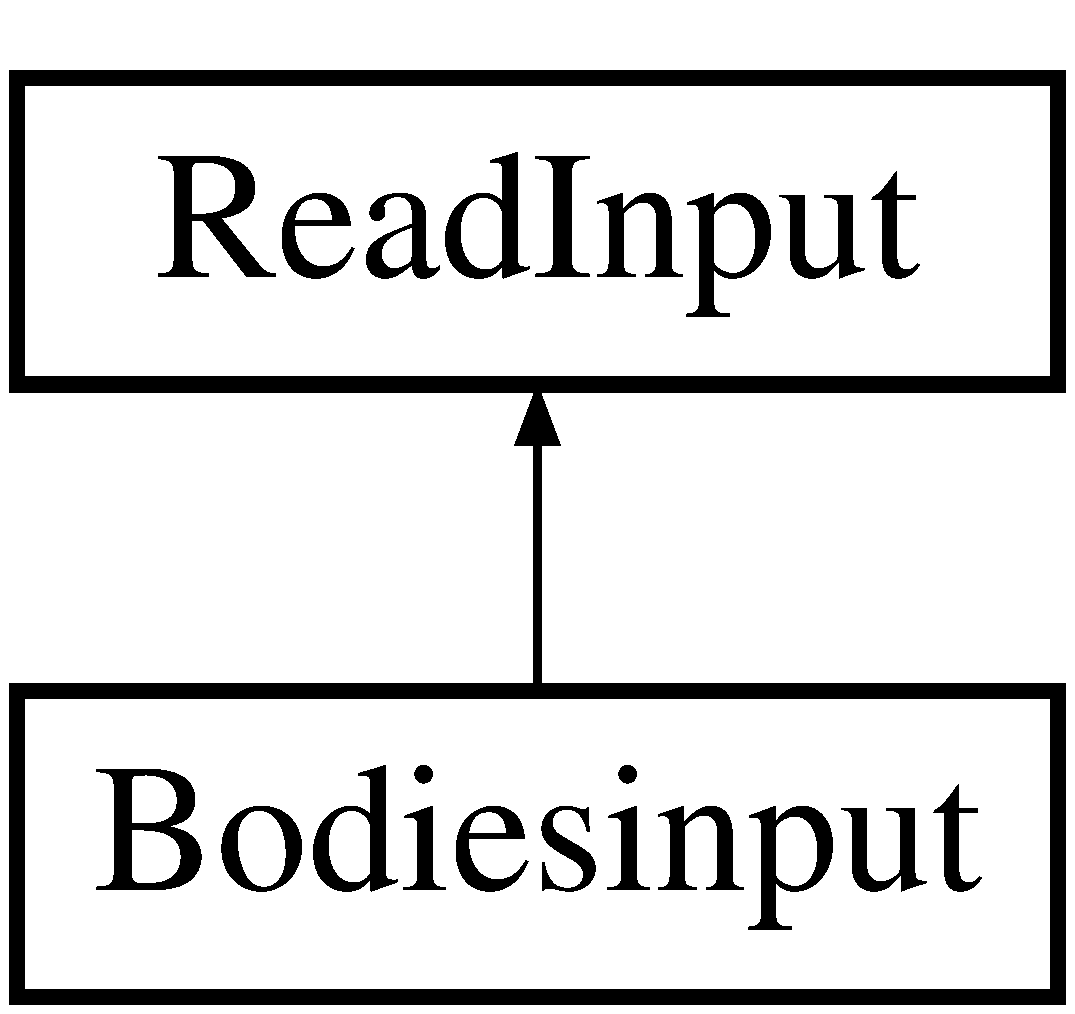
\includegraphics[height=2.000000cm]{class_bodiesinput}
\end{center}
\end{figure}
\subsection*{Public Member Functions}
\begin{DoxyCompactItemize}
\item 
\hyperlink{class_bodiesinput_a978009fcccf310bddf3ecb2261f7b9ed}{Bodiesinput} ()
\item 
\hyperlink{class_bodiesinput_ab478797f356b2d02c7be5a04c5e08d69}{$\sim$\-Bodiesinput} ()
\item 
void \hyperlink{class_bodiesinput_ab4dda6e4b858b9e349b5cc9ba155b4cd}{test\-Print} ()
\item 
vector$<$ \hyperlink{class_body}{Body} $>$ \& \hyperlink{class_bodiesinput_a0526664103347cd11e2b6fc15e8f8e61}{get\-Body\-Data} ()
\end{DoxyCompactItemize}
\subsection*{Protected Member Functions}
\begin{DoxyCompactItemize}
\item 
void \hyperlink{class_bodiesinput_ae7c0a7ee2c02e1ed63658a7d06f257e5}{initialize\-Defaults} ()
\item 
int \hyperlink{class_bodiesinput_abe777be6f9181f1d0f8c5ad523eff6e3}{legal\-Keyword} (string)
\item 
bool \hyperlink{class_bodiesinput_a2bf5785740ebd6e397477e667af16a05}{keyword\-Handler} (int, string, string)
\item 
bool \hyperlink{class_bodiesinput_af735a952cbd5b1a0c5db67c7209ba847}{keyword\-Handler} (int, vector$<$ string $>$, bool)
\item 
void \hyperlink{class_bodiesinput_a752cc5feeefe16345651b8133a132411}{add\-New\-Body} (string)
\end{DoxyCompactItemize}


\subsection{Detailed Description}
This class parses input from file and stores the data appropriately in the \hyperlink{class_body}{Body} object(s). 

\subsection{Constructor \& Destructor Documentation}
\hypertarget{class_bodiesinput_a978009fcccf310bddf3ecb2261f7b9ed}{\index{Bodiesinput@{Bodiesinput}!Bodiesinput@{Bodiesinput}}
\index{Bodiesinput@{Bodiesinput}!Bodiesinput@{Bodiesinput}}
\subsubsection[{Bodiesinput}]{\setlength{\rightskip}{0pt plus 5cm}Bodiesinput\-::\-Bodiesinput (
\begin{DoxyParamCaption}
{}
\end{DoxyParamCaption}
)}}\label{class_bodiesinput_a978009fcccf310bddf3ecb2261f7b9ed}
The default constructor. \hypertarget{class_bodiesinput_ab478797f356b2d02c7be5a04c5e08d69}{\index{Bodiesinput@{Bodiesinput}!$\sim$\-Bodiesinput@{$\sim$\-Bodiesinput}}
\index{$\sim$\-Bodiesinput@{$\sim$\-Bodiesinput}!Bodiesinput@{Bodiesinput}}
\subsubsection[{$\sim$\-Bodiesinput}]{\setlength{\rightskip}{0pt plus 5cm}Bodiesinput\-::$\sim$\-Bodiesinput (
\begin{DoxyParamCaption}
{}
\end{DoxyParamCaption}
)}}\label{class_bodiesinput_ab478797f356b2d02c7be5a04c5e08d69}
The default destructor, nothing happens here. 

\subsection{Member Function Documentation}
\hypertarget{class_bodiesinput_a752cc5feeefe16345651b8133a132411}{\index{Bodiesinput@{Bodiesinput}!add\-New\-Body@{add\-New\-Body}}
\index{add\-New\-Body@{add\-New\-Body}!Bodiesinput@{Bodiesinput}}
\subsubsection[{add\-New\-Body}]{\setlength{\rightskip}{0pt plus 5cm}void Bodiesinput\-::add\-New\-Body (
\begin{DoxyParamCaption}
\item[{string}]{new\-Name}
\end{DoxyParamCaption}
)\hspace{0.3cm}{\ttfamily [protected]}}}\label{class_bodiesinput_a752cc5feeefe16345651b8133a132411}
Adds a new body to the list. 
\begin{DoxyParams}{Parameters}
{\em new\-Name} & The name of the body to be added to the list. \\
\hline
\end{DoxyParams}
\hypertarget{class_bodiesinput_a0526664103347cd11e2b6fc15e8f8e61}{\index{Bodiesinput@{Bodiesinput}!get\-Body\-Data@{get\-Body\-Data}}
\index{get\-Body\-Data@{get\-Body\-Data}!Bodiesinput@{Bodiesinput}}
\subsubsection[{get\-Body\-Data}]{\setlength{\rightskip}{0pt plus 5cm}vector$<$ {\bf Body} $>$ \& Bodiesinput\-::get\-Body\-Data (
\begin{DoxyParamCaption}
{}
\end{DoxyParamCaption}
)}}\label{class_bodiesinput_a0526664103347cd11e2b6fc15e8f8e61}
Returns all bodies. \hypertarget{class_bodiesinput_ae7c0a7ee2c02e1ed63658a7d06f257e5}{\index{Bodiesinput@{Bodiesinput}!initialize\-Defaults@{initialize\-Defaults}}
\index{initialize\-Defaults@{initialize\-Defaults}!Bodiesinput@{Bodiesinput}}
\subsubsection[{initialize\-Defaults}]{\setlength{\rightskip}{0pt plus 5cm}void Bodiesinput\-::initialize\-Defaults (
\begin{DoxyParamCaption}
{}
\end{DoxyParamCaption}
)\hspace{0.3cm}{\ttfamily [protected]}, {\ttfamily [virtual]}}}\label{class_bodiesinput_ae7c0a7ee2c02e1ed63658a7d06f257e5}
For future use, does nothing as of now. 

Implements \hyperlink{class_read_input_a4ff2727b876cfd7c01299b08bdd65646}{Read\-Input}.

\hypertarget{class_bodiesinput_a2bf5785740ebd6e397477e667af16a05}{\index{Bodiesinput@{Bodiesinput}!keyword\-Handler@{keyword\-Handler}}
\index{keyword\-Handler@{keyword\-Handler}!Bodiesinput@{Bodiesinput}}
\subsubsection[{keyword\-Handler}]{\setlength{\rightskip}{0pt plus 5cm}bool Bodiesinput\-::keyword\-Handler (
\begin{DoxyParamCaption}
\item[{int}]{key\-Control, }
\item[{string}]{identifier, }
\item[{string}]{val}
\end{DoxyParamCaption}
)\hspace{0.3cm}{\ttfamily [protected]}, {\ttfamily [virtual]}}}\label{class_bodiesinput_a2bf5785740ebd6e397477e667af16a05}
Stores the data if valid keyword according to the legeal\-Keyword function. 
\begin{DoxyParams}{Parameters}
{\em key\-Control} & Indicated which case in switch function to use. \\
\hline
{\em identifier} & The keyword. \\
\hline
{\em val} & The value associated with the keyword. \\
\hline
\end{DoxyParams}
\begin{DoxyReturn}{Returns}
false if not done reading data, true to move onto next keyword in parser. 
\end{DoxyReturn}


Implements \hyperlink{class_read_input_a1d8cb0ef59f265300b682de97513f48d}{Read\-Input}.

\hypertarget{class_bodiesinput_af735a952cbd5b1a0c5db67c7209ba847}{\index{Bodiesinput@{Bodiesinput}!keyword\-Handler@{keyword\-Handler}}
\index{keyword\-Handler@{keyword\-Handler}!Bodiesinput@{Bodiesinput}}
\subsubsection[{keyword\-Handler}]{\setlength{\rightskip}{0pt plus 5cm}bool Bodiesinput\-::keyword\-Handler (
\begin{DoxyParamCaption}
\item[{int}]{key\-Control, }
\item[{vector$<$ string $>$}]{the\-List\-In, }
\item[{bool}]{is\-Direct}
\end{DoxyParamCaption}
)\hspace{0.3cm}{\ttfamily [protected]}, {\ttfamily [virtual]}}}\label{class_bodiesinput_af735a952cbd5b1a0c5db67c7209ba847}
Stores the list data if valid keyword according to the legeal\-Keyword function. 
\begin{DoxyParams}{Parameters}
{\em key\-Control} & Indicated which case in switch function to use. \\
\hline
{\em the\-List\-In} & List of Values. \\
\hline
{\em is\-Direct} & True if Direct Access List, False if Sequenctial List. \\
\hline
\end{DoxyParams}
\begin{DoxyReturn}{Returns}
false if not done reading data, true to move onto next keyword in parser. 
\end{DoxyReturn}


Implements \hyperlink{class_read_input_afb66a7ff67d0aeb10a3cfa5a4fbc31f8}{Read\-Input}.

\hypertarget{class_bodiesinput_abe777be6f9181f1d0f8c5ad523eff6e3}{\index{Bodiesinput@{Bodiesinput}!legal\-Keyword@{legal\-Keyword}}
\index{legal\-Keyword@{legal\-Keyword}!Bodiesinput@{Bodiesinput}}
\subsubsection[{legal\-Keyword}]{\setlength{\rightskip}{0pt plus 5cm}int Bodiesinput\-::legal\-Keyword (
\begin{DoxyParamCaption}
\item[{string}]{string\-In}
\end{DoxyParamCaption}
)\hspace{0.3cm}{\ttfamily [protected]}, {\ttfamily [virtual]}}}\label{class_bodiesinput_abe777be6f9181f1d0f8c5ad523eff6e3}
Returns int greater than 0 if the keyword is legal, the int returned specifies how to handle data in keyword\-Handler. 
\begin{DoxyParams}{Parameters}
{\em string\-In} & Check if a valid keyword. \\
\hline
\end{DoxyParams}
\begin{DoxyReturn}{Returns}
int value which tells keyword\-Handler how to handle the data. 
\end{DoxyReturn}


Implements \hyperlink{class_read_input_a4c67f10e813686bf635dd4c6bb2c61bc}{Read\-Input}.

\hypertarget{class_bodiesinput_ab4dda6e4b858b9e349b5cc9ba155b4cd}{\index{Bodiesinput@{Bodiesinput}!test\-Print@{test\-Print}}
\index{test\-Print@{test\-Print}!Bodiesinput@{Bodiesinput}}
\subsubsection[{test\-Print}]{\setlength{\rightskip}{0pt plus 5cm}void Bodiesinput\-::test\-Print (
\begin{DoxyParamCaption}
{}
\end{DoxyParamCaption}
)}}\label{class_bodiesinput_ab4dda6e4b858b9e349b5cc9ba155b4cd}
Print to console all data members. 

The documentation for this class was generated from the following files\-:\begin{DoxyCompactItemize}
\item 
Visual Studio 2010/\-Projects/o\-Freq Windows V\-S2010/o\-Freq/bodiesinput.\-h\item 
Visual Studio 2010/\-Projects/o\-Freq Windows V\-S2010/o\-Freq/bodiesinput.\-cpp\end{DoxyCompactItemize}

\hypertarget{class_body}{\section{Body Class Reference}
\label{class_body}\index{Body@{Body}}
}


{\ttfamily \#include $<$body.\-h$>$}

\subsection*{Public Member Functions}
\begin{DoxyCompactItemize}
\item 
\hyperlink{class_body_a7727b0d8c998bbc2942e4c802e31e2eb}{Body} ()
\item 
\hyperlink{class_body_abe1c4da65568cf7978b6247affc461e3}{$\sim$\-Body} ()
\item 
void \hyperlink{class_body_a31b959b6f30e3c9c6ebc3f0a325fec9d}{test\-Print} ()
\item 
void \hyperlink{class_body_a21190f9d796d631202db6caf768beae1}{set\-Body\-Name} (string)
\item 
void \hyperlink{class_body_ac2cb95c1a4d24e6b456db9bfe3e6dea3}{set\-Hydro\-Body\-Name} (string)
\item 
void \hyperlink{class_body_a7bba55a8fd4aea7a17ce7bd5f54d6ab8}{set\-Heading} (double)
\item 
void \hyperlink{class_body_a8165a9147387e4fc34757dab76e11117}{set\-Motion\-Model} (string)
\item 
void \hyperlink{class_body_aaa26153bd320830684e65bbf538b139d}{set\-User\-Active\-Forces} (vector$<$ string $>$)
\item 
void \hyperlink{class_body_aa3b532c91892c7336309df492cad39d6}{set\-User\-Reactive\-Forces} (vector$<$ string $>$)
\item 
void \hyperlink{class_body_af409e4b49b838e118a57a753879685dc}{set\-User\-Cross\-Body\-Forces} (vector$<$ string $>$)
\item 
void \hyperlink{class_body_a34950bfba0878d2488f91a0f5a1ae918}{set\-Hydro\-Active\-Forces} (vector$<$ string $>$)
\item 
void \hyperlink{class_body_ae26fc5ecce5fd1803ce26bf87d1d2a2b}{set\-Hydro\-Reactive\-Forces} (vector$<$ string $>$)
\item 
void \hyperlink{class_body_a47aed2abb4a77b9da93a803f7fdd5e31}{set\-Hydro\-Cross\-Body\-Forces} (vector$<$ string $>$)
\item 
void \hyperlink{class_body_a1bcd87df62f0cdd063c01799c1631ebd}{add\-Linked\-Body} (string)
\item 
void \hyperlink{class_body_a896b660a9d001422f5d2b0b4e6d77b98}{set\-Mass} (double)
\item 
void \hyperlink{class_body_a741a229a3671a7cf3d399a4e5d02596c}{set\-Moment\-X\-X} (double)
\item 
void \hyperlink{class_body_a06cdb969a55ebeff8d83ffcae66ab4ed}{set\-Moment\-Y\-Y} (double)
\item 
void \hyperlink{class_body_a270e3714cad10195b7dadc749727dba7}{set\-Moment\-Z\-Z} (double)
\item 
void \hyperlink{class_body_a24ddd15ae01d27675788658e65fcb199}{set\-Cross\-Moment\-X\-Y} (double)
\item 
void \hyperlink{class_body_a5f75e49f031e7b3dd711dd8e9d25eee8}{set\-Cross\-Moment\-X\-Z} (double)
\item 
void \hyperlink{class_body_ab99551cb3c2183db44ef86304b2e134b}{set\-Cross\-Moment\-Y\-Z} (double)
\item 
void \hyperlink{class_body_aca9af7a0a510f0a1ee9b0b29f7ed0217}{set\-Centroid\-X} (double)
\item 
void \hyperlink{class_body_a86f41f3de49b7e79c2387d92bb124204}{set\-Centroid\-Y} (double)
\item 
void \hyperlink{class_body_ad778b4919794533f12cfb93e818d5759}{set\-Centroid\-Z} (double)
\item 
void \hyperlink{class_body_a38933b2aec94873355dcecc8f8b41db2}{set\-Cross\-Body\-Name} (string)
\item 
string \hyperlink{class_body_ab4340cac445ae26ae751a08c35155386}{get\-Motion\-Model} ()
\item 
string \hyperlink{class_body_aab63febbe35984d8551a188b40ee3c3f}{get\-Body\-Name} ()
\end{DoxyCompactItemize}
\subsection*{Public Attributes}
\begin{DoxyCompactItemize}
\item 
vector$<$ string $>$ \hyperlink{class_body_a76e1e921e0cec08caed125073844c217}{user\-Active\-Forces}
\item 
vector$<$ string $>$ \hyperlink{class_body_af74f87986817f8c5cbd8408b29d04063}{user\-Reactive\-Forces}
\item 
vector$<$ string $>$ \hyperlink{class_body_a0ab89cfc3da49d74fa35ed90a0740e28}{user\-Cross\-Body\-Forces}
\item 
vector$<$ string $>$ \hyperlink{class_body_af307fb84335ee5e795b44595ce63015c}{hydro\-Active\-Forces}
\item 
vector$<$ string $>$ \hyperlink{class_body_a45e72e2a50d93068862b57bf4850a43b}{hydro\-Reactive\-Forces}
\item 
vector$<$ string $>$ \hyperlink{class_body_ad5ab2bc2f00fcb646a27398b0245696d}{hydro\-Cross\-Body\-Forces}
\item 
vector$<$ string $>$ \hyperlink{class_body_aabf9875fae852bd842d4b2b57d25eb73}{linked\-Body}
\item 
string \hyperlink{class_body_aa1ea62768021b84bb1c290c6bfaedbfe}{body\-Name}
\item 
string \hyperlink{class_body_a843782f1874dd366786864d9d3e0d9b7}{hydro\-Body}
\item 
string \hyperlink{class_body_a013a08fbeb1dd82131735dade5faa972}{motion\-Model}
\item 
double \hyperlink{class_body_abeaee44e6bc187426a1012bdaacb6eb4}{mass}
\item 
double \hyperlink{class_body_af29b06cfb14adbd1ad58d10a138a43c4}{moment\-Of\-Inertia\-X\-X}
\item 
double \hyperlink{class_body_adc1f40d6f14c7fea48f261170b8f4746}{moment\-Of\-Inertia\-Y\-Y}
\item 
double \hyperlink{class_body_a6f7c025addc1fd46cf72c18713a9cacf}{moment\-Of\-Inertia\-Z\-Z}
\item 
double \hyperlink{class_body_afd989f0185a85ef68120e88d6564631f}{cross\-Moment\-Of\-Inertia\-X\-Y}
\item 
double \hyperlink{class_body_a15c460e8cc8ae20b2420b379c0a6c760}{cross\-Moment\-Of\-Inertia\-X\-Z}
\item 
double \hyperlink{class_body_a552260d9dc6a203857955df8cc58662a}{cross\-Moment\-Of\-Inertia\-Y\-Z}
\item 
double \hyperlink{class_body_a5dc912a4a096590e90fd681a01ffc708}{centroid\-X}
\item 
double \hyperlink{class_body_aac1b166131421c882d1ec647b740c865}{centroid\-Y}
\item 
double \hyperlink{class_body_a834c22ac029cd86bc72185f027cdf74f}{centroid\-Z}
\item 
double \hyperlink{class_body_afe24a9330df6c053cc4fbbd03d477954}{heading}
\end{DoxyCompactItemize}


\subsection{Detailed Description}
This class holds all of the data for the \hyperlink{class_body}{Body} Input File. 

\subsection{Constructor \& Destructor Documentation}
\hypertarget{class_body_a7727b0d8c998bbc2942e4c802e31e2eb}{\index{Body@{Body}!Body@{Body}}
\index{Body@{Body}!Body@{Body}}
\subsubsection[{Body}]{\setlength{\rightskip}{0pt plus 5cm}Body\-::\-Body (
\begin{DoxyParamCaption}
{}
\end{DoxyParamCaption}
)}}\label{class_body_a7727b0d8c998bbc2942e4c802e31e2eb}
The default constructor \hypertarget{class_body_abe1c4da65568cf7978b6247affc461e3}{\index{Body@{Body}!$\sim$\-Body@{$\sim$\-Body}}
\index{$\sim$\-Body@{$\sim$\-Body}!Body@{Body}}
\subsubsection[{$\sim$\-Body}]{\setlength{\rightskip}{0pt plus 5cm}Body\-::$\sim$\-Body (
\begin{DoxyParamCaption}
{}
\end{DoxyParamCaption}
)}}\label{class_body_abe1c4da65568cf7978b6247affc461e3}
The default destructor, nothing happens here. 

\subsection{Member Function Documentation}
\hypertarget{class_body_a1bcd87df62f0cdd063c01799c1631ebd}{\index{Body@{Body}!add\-Linked\-Body@{add\-Linked\-Body}}
\index{add\-Linked\-Body@{add\-Linked\-Body}!Body@{Body}}
\subsubsection[{add\-Linked\-Body}]{\setlength{\rightskip}{0pt plus 5cm}void Body\-::add\-Linked\-Body (
\begin{DoxyParamCaption}
\item[{string}]{new\-Linked\-Body}
\end{DoxyParamCaption}
)}}\label{class_body_a1bcd87df62f0cdd063c01799c1631ebd}
Adds a linked body. 
\begin{DoxyParams}{Parameters}
{\em new\-Linked\-Body} & The string passed in is added to the linked\-Body vector. \\
\hline
\end{DoxyParams}
\hypertarget{class_body_aab63febbe35984d8551a188b40ee3c3f}{\index{Body@{Body}!get\-Body\-Name@{get\-Body\-Name}}
\index{get\-Body\-Name@{get\-Body\-Name}!Body@{Body}}
\subsubsection[{get\-Body\-Name}]{\setlength{\rightskip}{0pt plus 5cm}string Body\-::get\-Body\-Name (
\begin{DoxyParamCaption}
{}
\end{DoxyParamCaption}
)}}\label{class_body_aab63febbe35984d8551a188b40ee3c3f}
Get the name of the body. \begin{DoxyReturn}{Returns}
The name of the body. 
\end{DoxyReturn}
\hypertarget{class_body_ab4340cac445ae26ae751a08c35155386}{\index{Body@{Body}!get\-Motion\-Model@{get\-Motion\-Model}}
\index{get\-Motion\-Model@{get\-Motion\-Model}!Body@{Body}}
\subsubsection[{get\-Motion\-Model}]{\setlength{\rightskip}{0pt plus 5cm}string Body\-::get\-Motion\-Model (
\begin{DoxyParamCaption}
{}
\end{DoxyParamCaption}
)}}\label{class_body_ab4340cac445ae26ae751a08c35155386}
Get the name of the Motion Model. \begin{DoxyReturn}{Returns}
The string returned is the motion\-Model. 
\end{DoxyReturn}
\hypertarget{class_body_a21190f9d796d631202db6caf768beae1}{\index{Body@{Body}!set\-Body\-Name@{set\-Body\-Name}}
\index{set\-Body\-Name@{set\-Body\-Name}!Body@{Body}}
\subsubsection[{set\-Body\-Name}]{\setlength{\rightskip}{0pt plus 5cm}void Body\-::set\-Body\-Name (
\begin{DoxyParamCaption}
\item[{string}]{new\-Name}
\end{DoxyParamCaption}
)}}\label{class_body_a21190f9d796d631202db6caf768beae1}
Sets the body\-Name. 
\begin{DoxyParams}{Parameters}
{\em new\-Name} & The string passed in sets body\-Name. \\
\hline
\end{DoxyParams}
\hypertarget{class_body_aca9af7a0a510f0a1ee9b0b29f7ed0217}{\index{Body@{Body}!set\-Centroid\-X@{set\-Centroid\-X}}
\index{set\-Centroid\-X@{set\-Centroid\-X}!Body@{Body}}
\subsubsection[{set\-Centroid\-X}]{\setlength{\rightskip}{0pt plus 5cm}void Body\-::set\-Centroid\-X (
\begin{DoxyParamCaption}
\item[{double}]{new\-Cen\-X}
\end{DoxyParamCaption}
)}}\label{class_body_aca9af7a0a510f0a1ee9b0b29f7ed0217}
Sets the Centroid X. 
\begin{DoxyParams}{Parameters}
{\em new\-Cen\-X} & The double passed in sets centroid\-X. \\
\hline
\end{DoxyParams}
\hypertarget{class_body_a86f41f3de49b7e79c2387d92bb124204}{\index{Body@{Body}!set\-Centroid\-Y@{set\-Centroid\-Y}}
\index{set\-Centroid\-Y@{set\-Centroid\-Y}!Body@{Body}}
\subsubsection[{set\-Centroid\-Y}]{\setlength{\rightskip}{0pt plus 5cm}void Body\-::set\-Centroid\-Y (
\begin{DoxyParamCaption}
\item[{double}]{new\-Cen\-Y}
\end{DoxyParamCaption}
)}}\label{class_body_a86f41f3de49b7e79c2387d92bb124204}
Sets the Centroid Y. 
\begin{DoxyParams}{Parameters}
{\em new\-Cen\-Y} & The double passed in sets centroid\-Y. \\
\hline
\end{DoxyParams}
\hypertarget{class_body_ad778b4919794533f12cfb93e818d5759}{\index{Body@{Body}!set\-Centroid\-Z@{set\-Centroid\-Z}}
\index{set\-Centroid\-Z@{set\-Centroid\-Z}!Body@{Body}}
\subsubsection[{set\-Centroid\-Z}]{\setlength{\rightskip}{0pt plus 5cm}void Body\-::set\-Centroid\-Z (
\begin{DoxyParamCaption}
\item[{double}]{new\-Cen\-Z}
\end{DoxyParamCaption}
)}}\label{class_body_ad778b4919794533f12cfb93e818d5759}
Sets the Centroid Z. 
\begin{DoxyParams}{Parameters}
{\em new\-Cen\-Z} & The double passed in sets centroid\-Z. \\
\hline
\end{DoxyParams}
\hypertarget{class_body_a38933b2aec94873355dcecc8f8b41db2}{\index{Body@{Body}!set\-Cross\-Body\-Name@{set\-Cross\-Body\-Name}}
\index{set\-Cross\-Body\-Name@{set\-Cross\-Body\-Name}!Body@{Body}}
\subsubsection[{set\-Cross\-Body\-Name}]{\setlength{\rightskip}{0pt plus 5cm}void Body\-::set\-Cross\-Body\-Name (
\begin{DoxyParamCaption}
\item[{string}]{new\-Name}
\end{DoxyParamCaption}
)}}\label{class_body_a38933b2aec94873355dcecc8f8b41db2}
Adds a cross body name. 
\begin{DoxyParams}{Parameters}
{\em new\-Name} & The string passed in is added to the vector that holds the list of cross body forces. \\
\hline
\end{DoxyParams}
\hypertarget{class_body_a24ddd15ae01d27675788658e65fcb199}{\index{Body@{Body}!set\-Cross\-Moment\-X\-Y@{set\-Cross\-Moment\-X\-Y}}
\index{set\-Cross\-Moment\-X\-Y@{set\-Cross\-Moment\-X\-Y}!Body@{Body}}
\subsubsection[{set\-Cross\-Moment\-X\-Y}]{\setlength{\rightskip}{0pt plus 5cm}void Body\-::set\-Cross\-Moment\-X\-Y (
\begin{DoxyParamCaption}
\item[{double}]{new\-X\-Y}
\end{DoxyParamCaption}
)}}\label{class_body_a24ddd15ae01d27675788658e65fcb199}
Sets the Product of Inertia X\-Y (Ixy) 
\begin{DoxyParams}{Parameters}
{\em new\-X\-Y} & The double passed in sets set\-Cross\-Moment\-X\-Y. \\
\hline
\end{DoxyParams}
\hypertarget{class_body_a5f75e49f031e7b3dd711dd8e9d25eee8}{\index{Body@{Body}!set\-Cross\-Moment\-X\-Z@{set\-Cross\-Moment\-X\-Z}}
\index{set\-Cross\-Moment\-X\-Z@{set\-Cross\-Moment\-X\-Z}!Body@{Body}}
\subsubsection[{set\-Cross\-Moment\-X\-Z}]{\setlength{\rightskip}{0pt plus 5cm}void Body\-::set\-Cross\-Moment\-X\-Z (
\begin{DoxyParamCaption}
\item[{double}]{new\-X\-Z}
\end{DoxyParamCaption}
)}}\label{class_body_a5f75e49f031e7b3dd711dd8e9d25eee8}
Sets the Product of Inertia X\-Z (Ixz) 
\begin{DoxyParams}{Parameters}
{\em new\-X\-Z} & The double passed in sets set\-Cross\-Moment\-X\-Z. \\
\hline
\end{DoxyParams}
\hypertarget{class_body_ab99551cb3c2183db44ef86304b2e134b}{\index{Body@{Body}!set\-Cross\-Moment\-Y\-Z@{set\-Cross\-Moment\-Y\-Z}}
\index{set\-Cross\-Moment\-Y\-Z@{set\-Cross\-Moment\-Y\-Z}!Body@{Body}}
\subsubsection[{set\-Cross\-Moment\-Y\-Z}]{\setlength{\rightskip}{0pt plus 5cm}void Body\-::set\-Cross\-Moment\-Y\-Z (
\begin{DoxyParamCaption}
\item[{double}]{new\-Y\-Z}
\end{DoxyParamCaption}
)}}\label{class_body_ab99551cb3c2183db44ef86304b2e134b}
Sets the Product of Inertia Y\-Z (Iyz) 
\begin{DoxyParams}{Parameters}
{\em new\-Y\-Z} & The double passed in sets set\-Cross\-Moment\-Y\-Z. \\
\hline
\end{DoxyParams}
\hypertarget{class_body_a7bba55a8fd4aea7a17ce7bd5f54d6ab8}{\index{Body@{Body}!set\-Heading@{set\-Heading}}
\index{set\-Heading@{set\-Heading}!Body@{Body}}
\subsubsection[{set\-Heading}]{\setlength{\rightskip}{0pt plus 5cm}void Body\-::set\-Heading (
\begin{DoxyParamCaption}
\item[{double}]{new\-Heading}
\end{DoxyParamCaption}
)}}\label{class_body_a7bba55a8fd4aea7a17ce7bd5f54d6ab8}
Sets the heading. 
\begin{DoxyParams}{Parameters}
{\em new\-Heading} & The double passed in sets the heading. \\
\hline
\end{DoxyParams}
\hypertarget{class_body_a34950bfba0878d2488f91a0f5a1ae918}{\index{Body@{Body}!set\-Hydro\-Active\-Forces@{set\-Hydro\-Active\-Forces}}
\index{set\-Hydro\-Active\-Forces@{set\-Hydro\-Active\-Forces}!Body@{Body}}
\subsubsection[{set\-Hydro\-Active\-Forces}]{\setlength{\rightskip}{0pt plus 5cm}void Body\-::set\-Hydro\-Active\-Forces (
\begin{DoxyParamCaption}
\item[{vector$<$ string $>$}]{new\-Force\-List}
\end{DoxyParamCaption}
)}}\label{class_body_a34950bfba0878d2488f91a0f5a1ae918}
Sets the hydro active forces. 
\begin{DoxyParams}{Parameters}
{\em new\-Force\-List} & The vector of strings sets hydro\-Active\-Forces. \\
\hline
\end{DoxyParams}
\hypertarget{class_body_ac2cb95c1a4d24e6b456db9bfe3e6dea3}{\index{Body@{Body}!set\-Hydro\-Body\-Name@{set\-Hydro\-Body\-Name}}
\index{set\-Hydro\-Body\-Name@{set\-Hydro\-Body\-Name}!Body@{Body}}
\subsubsection[{set\-Hydro\-Body\-Name}]{\setlength{\rightskip}{0pt plus 5cm}void Body\-::set\-Hydro\-Body\-Name (
\begin{DoxyParamCaption}
\item[{string}]{new\-Name}
\end{DoxyParamCaption}
)}}\label{class_body_ac2cb95c1a4d24e6b456db9bfe3e6dea3}
Sets the hydro\-Body. 
\begin{DoxyParams}{Parameters}
{\em new\-Name} & The string passed in sets the hydro\-Body. \\
\hline
\end{DoxyParams}
\hypertarget{class_body_a47aed2abb4a77b9da93a803f7fdd5e31}{\index{Body@{Body}!set\-Hydro\-Cross\-Body\-Forces@{set\-Hydro\-Cross\-Body\-Forces}}
\index{set\-Hydro\-Cross\-Body\-Forces@{set\-Hydro\-Cross\-Body\-Forces}!Body@{Body}}
\subsubsection[{set\-Hydro\-Cross\-Body\-Forces}]{\setlength{\rightskip}{0pt plus 5cm}void Body\-::set\-Hydro\-Cross\-Body\-Forces (
\begin{DoxyParamCaption}
\item[{vector$<$ string $>$}]{new\-Force\-List}
\end{DoxyParamCaption}
)}}\label{class_body_a47aed2abb4a77b9da93a803f7fdd5e31}
Sets the hydro active forces. 
\begin{DoxyParams}{Parameters}
{\em new\-Force\-List} & The vector of strings sets hydro\-Cross\-Body\-Forces. \\
\hline
\end{DoxyParams}
\hypertarget{class_body_ae26fc5ecce5fd1803ce26bf87d1d2a2b}{\index{Body@{Body}!set\-Hydro\-Reactive\-Forces@{set\-Hydro\-Reactive\-Forces}}
\index{set\-Hydro\-Reactive\-Forces@{set\-Hydro\-Reactive\-Forces}!Body@{Body}}
\subsubsection[{set\-Hydro\-Reactive\-Forces}]{\setlength{\rightskip}{0pt plus 5cm}void Body\-::set\-Hydro\-Reactive\-Forces (
\begin{DoxyParamCaption}
\item[{vector$<$ string $>$}]{new\-Force\-List}
\end{DoxyParamCaption}
)}}\label{class_body_ae26fc5ecce5fd1803ce26bf87d1d2a2b}
Sets the hydro reactive forces. 
\begin{DoxyParams}{Parameters}
{\em new\-Force\-List} & The vector of strings sets hydro\-Reactive\-Force. \\
\hline
\end{DoxyParams}
\hypertarget{class_body_a896b660a9d001422f5d2b0b4e6d77b98}{\index{Body@{Body}!set\-Mass@{set\-Mass}}
\index{set\-Mass@{set\-Mass}!Body@{Body}}
\subsubsection[{set\-Mass}]{\setlength{\rightskip}{0pt plus 5cm}void Body\-::set\-Mass (
\begin{DoxyParamCaption}
\item[{double}]{new\-Mass}
\end{DoxyParamCaption}
)}}\label{class_body_a896b660a9d001422f5d2b0b4e6d77b98}
Sets the mass. 
\begin{DoxyParams}{Parameters}
{\em new\-Mass} & The double passed in sets the mass. \\
\hline
\end{DoxyParams}
\hypertarget{class_body_a741a229a3671a7cf3d399a4e5d02596c}{\index{Body@{Body}!set\-Moment\-X\-X@{set\-Moment\-X\-X}}
\index{set\-Moment\-X\-X@{set\-Moment\-X\-X}!Body@{Body}}
\subsubsection[{set\-Moment\-X\-X}]{\setlength{\rightskip}{0pt plus 5cm}void Body\-::set\-Moment\-X\-X (
\begin{DoxyParamCaption}
\item[{double}]{new\-X\-X}
\end{DoxyParamCaption}
)}}\label{class_body_a741a229a3671a7cf3d399a4e5d02596c}
Sets the Moment of Inertia X\-X (Ixx) 
\begin{DoxyParams}{Parameters}
{\em new\-X\-X} & The double passed in sets moment\-Of\-Inertia\-X\-X. \\
\hline
\end{DoxyParams}
\hypertarget{class_body_a06cdb969a55ebeff8d83ffcae66ab4ed}{\index{Body@{Body}!set\-Moment\-Y\-Y@{set\-Moment\-Y\-Y}}
\index{set\-Moment\-Y\-Y@{set\-Moment\-Y\-Y}!Body@{Body}}
\subsubsection[{set\-Moment\-Y\-Y}]{\setlength{\rightskip}{0pt plus 5cm}void Body\-::set\-Moment\-Y\-Y (
\begin{DoxyParamCaption}
\item[{double}]{new\-Y\-Y}
\end{DoxyParamCaption}
)}}\label{class_body_a06cdb969a55ebeff8d83ffcae66ab4ed}
Sets the Moment of Inertia Y\-Y (Iyy) 
\begin{DoxyParams}{Parameters}
{\em new\-Y\-Y} & The double passed in sets moment\-Of\-Inertia\-Y\-Y. \\
\hline
\end{DoxyParams}
\hypertarget{class_body_a270e3714cad10195b7dadc749727dba7}{\index{Body@{Body}!set\-Moment\-Z\-Z@{set\-Moment\-Z\-Z}}
\index{set\-Moment\-Z\-Z@{set\-Moment\-Z\-Z}!Body@{Body}}
\subsubsection[{set\-Moment\-Z\-Z}]{\setlength{\rightskip}{0pt plus 5cm}void Body\-::set\-Moment\-Z\-Z (
\begin{DoxyParamCaption}
\item[{double}]{new\-Z\-Z}
\end{DoxyParamCaption}
)}}\label{class_body_a270e3714cad10195b7dadc749727dba7}
Sets the Moment of Inertia Z\-Z (Izz) 
\begin{DoxyParams}{Parameters}
{\em new\-Z\-Z} & The double passed in sets moment\-Of\-Inertia\-Z\-Z. \\
\hline
\end{DoxyParams}
\hypertarget{class_body_a8165a9147387e4fc34757dab76e11117}{\index{Body@{Body}!set\-Motion\-Model@{set\-Motion\-Model}}
\index{set\-Motion\-Model@{set\-Motion\-Model}!Body@{Body}}
\subsubsection[{set\-Motion\-Model}]{\setlength{\rightskip}{0pt plus 5cm}void Body\-::set\-Motion\-Model (
\begin{DoxyParamCaption}
\item[{string}]{new\-Motion\-Model}
\end{DoxyParamCaption}
)}}\label{class_body_a8165a9147387e4fc34757dab76e11117}
Sets the motion model. 
\begin{DoxyParams}{Parameters}
{\em new\-Motion\-Model} & The string passeed in sets the motion\-Model. \\
\hline
\end{DoxyParams}
\hypertarget{class_body_aaa26153bd320830684e65bbf538b139d}{\index{Body@{Body}!set\-User\-Active\-Forces@{set\-User\-Active\-Forces}}
\index{set\-User\-Active\-Forces@{set\-User\-Active\-Forces}!Body@{Body}}
\subsubsection[{set\-User\-Active\-Forces}]{\setlength{\rightskip}{0pt plus 5cm}void Body\-::set\-User\-Active\-Forces (
\begin{DoxyParamCaption}
\item[{vector$<$ string $>$}]{new\-Force\-List}
\end{DoxyParamCaption}
)}}\label{class_body_aaa26153bd320830684e65bbf538b139d}
Sets the user active forces. 
\begin{DoxyParams}{Parameters}
{\em new\-Force\-List} & The vector of strings sets user\-Active\-Forces. \\
\hline
\end{DoxyParams}
\hypertarget{class_body_af409e4b49b838e118a57a753879685dc}{\index{Body@{Body}!set\-User\-Cross\-Body\-Forces@{set\-User\-Cross\-Body\-Forces}}
\index{set\-User\-Cross\-Body\-Forces@{set\-User\-Cross\-Body\-Forces}!Body@{Body}}
\subsubsection[{set\-User\-Cross\-Body\-Forces}]{\setlength{\rightskip}{0pt plus 5cm}void Body\-::set\-User\-Cross\-Body\-Forces (
\begin{DoxyParamCaption}
\item[{vector$<$ string $>$}]{new\-Cross\-Body\-List}
\end{DoxyParamCaption}
)}}\label{class_body_af409e4b49b838e118a57a753879685dc}
Sets the user cross body forces. 
\begin{DoxyParams}{Parameters}
{\em new\-Cross\-Body\-List} & The vector of strings sets user\-Cross\-Body\-Forces. \\
\hline
\end{DoxyParams}
\hypertarget{class_body_aa3b532c91892c7336309df492cad39d6}{\index{Body@{Body}!set\-User\-Reactive\-Forces@{set\-User\-Reactive\-Forces}}
\index{set\-User\-Reactive\-Forces@{set\-User\-Reactive\-Forces}!Body@{Body}}
\subsubsection[{set\-User\-Reactive\-Forces}]{\setlength{\rightskip}{0pt plus 5cm}void Body\-::set\-User\-Reactive\-Forces (
\begin{DoxyParamCaption}
\item[{vector$<$ string $>$}]{new\-Force\-List}
\end{DoxyParamCaption}
)}}\label{class_body_aa3b532c91892c7336309df492cad39d6}
Sets the user reactive forces. 
\begin{DoxyParams}{Parameters}
{\em new\-Force\-List} & The vector of strings sets user\-Reactive\-Forces. \\
\hline
\end{DoxyParams}
\hypertarget{class_body_a31b959b6f30e3c9c6ebc3f0a325fec9d}{\index{Body@{Body}!test\-Print@{test\-Print}}
\index{test\-Print@{test\-Print}!Body@{Body}}
\subsubsection[{test\-Print}]{\setlength{\rightskip}{0pt plus 5cm}void Body\-::test\-Print (
\begin{DoxyParamCaption}
{}
\end{DoxyParamCaption}
)}}\label{class_body_a31b959b6f30e3c9c6ebc3f0a325fec9d}
Test print to console the values of all data members. 

\subsection{Member Data Documentation}
\hypertarget{class_body_aa1ea62768021b84bb1c290c6bfaedbfe}{\index{Body@{Body}!body\-Name@{body\-Name}}
\index{body\-Name@{body\-Name}!Body@{Body}}
\subsubsection[{body\-Name}]{\setlength{\rightskip}{0pt plus 5cm}string Body\-::body\-Name}}\label{class_body_aa1ea62768021b84bb1c290c6bfaedbfe}
The name of this body object. \hypertarget{class_body_a5dc912a4a096590e90fd681a01ffc708}{\index{Body@{Body}!centroid\-X@{centroid\-X}}
\index{centroid\-X@{centroid\-X}!Body@{Body}}
\subsubsection[{centroid\-X}]{\setlength{\rightskip}{0pt plus 5cm}double Body\-::centroid\-X}}\label{class_body_a5dc912a4a096590e90fd681a01ffc708}
Centroid X. \hypertarget{class_body_aac1b166131421c882d1ec647b740c865}{\index{Body@{Body}!centroid\-Y@{centroid\-Y}}
\index{centroid\-Y@{centroid\-Y}!Body@{Body}}
\subsubsection[{centroid\-Y}]{\setlength{\rightskip}{0pt plus 5cm}double Body\-::centroid\-Y}}\label{class_body_aac1b166131421c882d1ec647b740c865}
Centroid Y. \hypertarget{class_body_a834c22ac029cd86bc72185f027cdf74f}{\index{Body@{Body}!centroid\-Z@{centroid\-Z}}
\index{centroid\-Z@{centroid\-Z}!Body@{Body}}
\subsubsection[{centroid\-Z}]{\setlength{\rightskip}{0pt plus 5cm}double Body\-::centroid\-Z}}\label{class_body_a834c22ac029cd86bc72185f027cdf74f}
Centroid Z. \hypertarget{class_body_afd989f0185a85ef68120e88d6564631f}{\index{Body@{Body}!cross\-Moment\-Of\-Inertia\-X\-Y@{cross\-Moment\-Of\-Inertia\-X\-Y}}
\index{cross\-Moment\-Of\-Inertia\-X\-Y@{cross\-Moment\-Of\-Inertia\-X\-Y}!Body@{Body}}
\subsubsection[{cross\-Moment\-Of\-Inertia\-X\-Y}]{\setlength{\rightskip}{0pt plus 5cm}double Body\-::cross\-Moment\-Of\-Inertia\-X\-Y}}\label{class_body_afd989f0185a85ef68120e88d6564631f}
Product of Inertia X\-Y (Ixy). \hypertarget{class_body_a15c460e8cc8ae20b2420b379c0a6c760}{\index{Body@{Body}!cross\-Moment\-Of\-Inertia\-X\-Z@{cross\-Moment\-Of\-Inertia\-X\-Z}}
\index{cross\-Moment\-Of\-Inertia\-X\-Z@{cross\-Moment\-Of\-Inertia\-X\-Z}!Body@{Body}}
\subsubsection[{cross\-Moment\-Of\-Inertia\-X\-Z}]{\setlength{\rightskip}{0pt plus 5cm}double Body\-::cross\-Moment\-Of\-Inertia\-X\-Z}}\label{class_body_a15c460e8cc8ae20b2420b379c0a6c760}
Product of Inertia X\-Z (Ixz). \hypertarget{class_body_a552260d9dc6a203857955df8cc58662a}{\index{Body@{Body}!cross\-Moment\-Of\-Inertia\-Y\-Z@{cross\-Moment\-Of\-Inertia\-Y\-Z}}
\index{cross\-Moment\-Of\-Inertia\-Y\-Z@{cross\-Moment\-Of\-Inertia\-Y\-Z}!Body@{Body}}
\subsubsection[{cross\-Moment\-Of\-Inertia\-Y\-Z}]{\setlength{\rightskip}{0pt plus 5cm}double Body\-::cross\-Moment\-Of\-Inertia\-Y\-Z}}\label{class_body_a552260d9dc6a203857955df8cc58662a}
Product of Inertia Y\-Z (Iyz). \hypertarget{class_body_afe24a9330df6c053cc4fbbd03d477954}{\index{Body@{Body}!heading@{heading}}
\index{heading@{heading}!Body@{Body}}
\subsubsection[{heading}]{\setlength{\rightskip}{0pt plus 5cm}double Body\-::heading}}\label{class_body_afe24a9330df6c053cc4fbbd03d477954}
Heading. \hypertarget{class_body_af307fb84335ee5e795b44595ce63015c}{\index{Body@{Body}!hydro\-Active\-Forces@{hydro\-Active\-Forces}}
\index{hydro\-Active\-Forces@{hydro\-Active\-Forces}!Body@{Body}}
\subsubsection[{hydro\-Active\-Forces}]{\setlength{\rightskip}{0pt plus 5cm}vector$<$string$>$ Body\-::hydro\-Active\-Forces}}\label{class_body_af307fb84335ee5e795b44595ce63015c}
Holds the hydro active forces. \hypertarget{class_body_a843782f1874dd366786864d9d3e0d9b7}{\index{Body@{Body}!hydro\-Body@{hydro\-Body}}
\index{hydro\-Body@{hydro\-Body}!Body@{Body}}
\subsubsection[{hydro\-Body}]{\setlength{\rightskip}{0pt plus 5cm}string Body\-::hydro\-Body}}\label{class_body_a843782f1874dd366786864d9d3e0d9b7}
The name of this hydro body object. \hypertarget{class_body_ad5ab2bc2f00fcb646a27398b0245696d}{\index{Body@{Body}!hydro\-Cross\-Body\-Forces@{hydro\-Cross\-Body\-Forces}}
\index{hydro\-Cross\-Body\-Forces@{hydro\-Cross\-Body\-Forces}!Body@{Body}}
\subsubsection[{hydro\-Cross\-Body\-Forces}]{\setlength{\rightskip}{0pt plus 5cm}vector$<$string$>$ Body\-::hydro\-Cross\-Body\-Forces}}\label{class_body_ad5ab2bc2f00fcb646a27398b0245696d}
Holds the hydro cross body forces. \hypertarget{class_body_a45e72e2a50d93068862b57bf4850a43b}{\index{Body@{Body}!hydro\-Reactive\-Forces@{hydro\-Reactive\-Forces}}
\index{hydro\-Reactive\-Forces@{hydro\-Reactive\-Forces}!Body@{Body}}
\subsubsection[{hydro\-Reactive\-Forces}]{\setlength{\rightskip}{0pt plus 5cm}vector$<$string$>$ Body\-::hydro\-Reactive\-Forces}}\label{class_body_a45e72e2a50d93068862b57bf4850a43b}
Holds the hydro reactive forces. \hypertarget{class_body_aabf9875fae852bd842d4b2b57d25eb73}{\index{Body@{Body}!linked\-Body@{linked\-Body}}
\index{linked\-Body@{linked\-Body}!Body@{Body}}
\subsubsection[{linked\-Body}]{\setlength{\rightskip}{0pt plus 5cm}vector$<$string$>$ Body\-::linked\-Body}}\label{class_body_aabf9875fae852bd842d4b2b57d25eb73}
Holds a list of the linked bodies. \hypertarget{class_body_abeaee44e6bc187426a1012bdaacb6eb4}{\index{Body@{Body}!mass@{mass}}
\index{mass@{mass}!Body@{Body}}
\subsubsection[{mass}]{\setlength{\rightskip}{0pt plus 5cm}double Body\-::mass}}\label{class_body_abeaee44e6bc187426a1012bdaacb6eb4}
The mass. \hypertarget{class_body_af29b06cfb14adbd1ad58d10a138a43c4}{\index{Body@{Body}!moment\-Of\-Inertia\-X\-X@{moment\-Of\-Inertia\-X\-X}}
\index{moment\-Of\-Inertia\-X\-X@{moment\-Of\-Inertia\-X\-X}!Body@{Body}}
\subsubsection[{moment\-Of\-Inertia\-X\-X}]{\setlength{\rightskip}{0pt plus 5cm}double Body\-::moment\-Of\-Inertia\-X\-X}}\label{class_body_af29b06cfb14adbd1ad58d10a138a43c4}
Moment of Inertia X\-X (Ixx). \hypertarget{class_body_adc1f40d6f14c7fea48f261170b8f4746}{\index{Body@{Body}!moment\-Of\-Inertia\-Y\-Y@{moment\-Of\-Inertia\-Y\-Y}}
\index{moment\-Of\-Inertia\-Y\-Y@{moment\-Of\-Inertia\-Y\-Y}!Body@{Body}}
\subsubsection[{moment\-Of\-Inertia\-Y\-Y}]{\setlength{\rightskip}{0pt plus 5cm}double Body\-::moment\-Of\-Inertia\-Y\-Y}}\label{class_body_adc1f40d6f14c7fea48f261170b8f4746}
Moment of Inertia Y\-Y (Iyy). \hypertarget{class_body_a6f7c025addc1fd46cf72c18713a9cacf}{\index{Body@{Body}!moment\-Of\-Inertia\-Z\-Z@{moment\-Of\-Inertia\-Z\-Z}}
\index{moment\-Of\-Inertia\-Z\-Z@{moment\-Of\-Inertia\-Z\-Z}!Body@{Body}}
\subsubsection[{moment\-Of\-Inertia\-Z\-Z}]{\setlength{\rightskip}{0pt plus 5cm}double Body\-::moment\-Of\-Inertia\-Z\-Z}}\label{class_body_a6f7c025addc1fd46cf72c18713a9cacf}
Moment of Inertia Z\-Z (Izz). \hypertarget{class_body_a013a08fbeb1dd82131735dade5faa972}{\index{Body@{Body}!motion\-Model@{motion\-Model}}
\index{motion\-Model@{motion\-Model}!Body@{Body}}
\subsubsection[{motion\-Model}]{\setlength{\rightskip}{0pt plus 5cm}string Body\-::motion\-Model}}\label{class_body_a013a08fbeb1dd82131735dade5faa972}
The name of the motion model used for this body. \hypertarget{class_body_a76e1e921e0cec08caed125073844c217}{\index{Body@{Body}!user\-Active\-Forces@{user\-Active\-Forces}}
\index{user\-Active\-Forces@{user\-Active\-Forces}!Body@{Body}}
\subsubsection[{user\-Active\-Forces}]{\setlength{\rightskip}{0pt plus 5cm}vector$<$string$>$ Body\-::user\-Active\-Forces}}\label{class_body_a76e1e921e0cec08caed125073844c217}
Holds the user active forces. \hypertarget{class_body_a0ab89cfc3da49d74fa35ed90a0740e28}{\index{Body@{Body}!user\-Cross\-Body\-Forces@{user\-Cross\-Body\-Forces}}
\index{user\-Cross\-Body\-Forces@{user\-Cross\-Body\-Forces}!Body@{Body}}
\subsubsection[{user\-Cross\-Body\-Forces}]{\setlength{\rightskip}{0pt plus 5cm}vector$<$string$>$ Body\-::user\-Cross\-Body\-Forces}}\label{class_body_a0ab89cfc3da49d74fa35ed90a0740e28}
Holds the user cross body forces. \hypertarget{class_body_af74f87986817f8c5cbd8408b29d04063}{\index{Body@{Body}!user\-Reactive\-Forces@{user\-Reactive\-Forces}}
\index{user\-Reactive\-Forces@{user\-Reactive\-Forces}!Body@{Body}}
\subsubsection[{user\-Reactive\-Forces}]{\setlength{\rightskip}{0pt plus 5cm}vector$<$string$>$ Body\-::user\-Reactive\-Forces}}\label{class_body_af74f87986817f8c5cbd8408b29d04063}
Holds the user reactive forces. 

The documentation for this class was generated from the following files\-:\begin{DoxyCompactItemize}
\item 
Visual Studio 2010/\-Projects/o\-Freq Windows V\-S2010/o\-Freq/body.\-h\item 
Visual Studio 2010/\-Projects/o\-Freq Windows V\-S2010/o\-Freq/body.\-cpp\end{DoxyCompactItemize}

\hypertarget{class_body_with_force_matrix}{\section{Body\-With\-Force\-Matrix Class Reference}
\label{class_body_with_force_matrix}\index{Body\-With\-Force\-Matrix@{Body\-With\-Force\-Matrix}}
}
\subsection*{Public Member Functions}
\begin{DoxyCompactItemize}
\item 
\hyperlink{class_body_with_force_matrix_ac3c8391555c45e0a7eab476bf3488ae0}{Body\-With\-Force\-Matrix} ()
\item 
\hyperlink{class_body_with_force_matrix_a075b1ba0f74b27588f3e9affb7b9bb9e}{Body\-With\-Force\-Matrix} (\hyperlink{class_body}{Body}, \hyperlink{class_user_forces}{User\-Forces})
\item 
\hyperlink{class_body_with_force_matrix_a3eef8f497f99e49af7264a49a48a945d}{$\sim$\-Body\-With\-Force\-Matrix} ()
\end{DoxyCompactItemize}
\subsection*{Public Attributes}
\begin{DoxyCompactItemize}
\item 
cx\-\_\-mat \hyperlink{class_body_with_force_matrix_a3b07fb8ac7d58c1ed2b642676e51de6f}{mass\-Matrix}
\item 
vector$<$ \hyperlink{class_reactive_force_matrix}{Reactive\-Force\-Matrix} $>$ \hyperlink{class_body_with_force_matrix_a301fe6541bda12f4786c254688b1b89f}{user\-Reactive\-Force\-Matrix}
\item 
vector$<$ \hyperlink{class_reactive_force_matrix}{Reactive\-Force\-Matrix} $>$ \hyperlink{class_body_with_force_matrix_ad04bf64c3495a2d316f4ede7e6e307d3}{user\-Cross\-Body\-Force\-Matrix}
\item 
vector$<$ cx\-\_\-mat $>$ \hyperlink{class_body_with_force_matrix_aeb11660f006b6e86e8fc691bf55ce346}{user\-Active\-Force\-Matrix}
\item 
vector$<$ \hyperlink{class_reactive_force_matrix}{Reactive\-Force\-Matrix} $>$ \hyperlink{class_body_with_force_matrix_ab9be7a7eb8a4772ca011586590cfcbed}{hydro\-Reactive\-Force\-Matrix}
\item 
vector$<$ \hyperlink{class_reactive_force_matrix}{Reactive\-Force\-Matrix} $>$ \hyperlink{class_body_with_force_matrix_a0fe089e2b9d9bacaf38d8e2e957ee125}{hydro\-Cross\-Body\-Force\-Matrix}
\item 
vector$<$ cx\-\_\-mat $>$ \hyperlink{class_body_with_force_matrix_a8902e9ad82255e0794dff72725928ff9}{hydro\-Active\-Force\-Matrix}
\item 
vector$<$ string $>$ \hyperlink{class_body_with_force_matrix_adff7e3220bdcf4e367a5626afad29572}{user\-Active\-Force}
\item 
vector$<$ string $>$ \hyperlink{class_body_with_force_matrix_ad334068959cd4ad8591c31ff9d16225f}{user\-Reactive\-Force}
\item 
vector$<$ string $>$ \hyperlink{class_body_with_force_matrix_ad97183b090f4f9a1010bcfe028ec55b6}{user\-Cross\-Body\-Forces}
\item 
vector$<$ string $>$ \hyperlink{class_body_with_force_matrix_abab87c2d9bad9c11e526aa35fbe242cb}{hydro\-Active\-Force}
\item 
vector$<$ string $>$ \hyperlink{class_body_with_force_matrix_ade2cce8108c19527e229f960b7bf7cd1}{hydro\-Reactive\-Force}
\item 
vector$<$ string $>$ \hyperlink{class_body_with_force_matrix_ae43f824670c354999843f2cc3e0987c8}{hydro\-Cross\-Body\-Forces}
\end{DoxyCompactItemize}


\subsection{Constructor \& Destructor Documentation}
\hypertarget{class_body_with_force_matrix_ac3c8391555c45e0a7eab476bf3488ae0}{\index{Body\-With\-Force\-Matrix@{Body\-With\-Force\-Matrix}!Body\-With\-Force\-Matrix@{Body\-With\-Force\-Matrix}}
\index{Body\-With\-Force\-Matrix@{Body\-With\-Force\-Matrix}!BodyWithForceMatrix@{Body\-With\-Force\-Matrix}}
\subsubsection[{Body\-With\-Force\-Matrix}]{\setlength{\rightskip}{0pt plus 5cm}Body\-With\-Force\-Matrix\-::\-Body\-With\-Force\-Matrix (
\begin{DoxyParamCaption}
{}
\end{DoxyParamCaption}
)}}\label{class_body_with_force_matrix_ac3c8391555c45e0a7eab476bf3488ae0}
The default constructor. \hypertarget{class_body_with_force_matrix_a075b1ba0f74b27588f3e9affb7b9bb9e}{\index{Body\-With\-Force\-Matrix@{Body\-With\-Force\-Matrix}!Body\-With\-Force\-Matrix@{Body\-With\-Force\-Matrix}}
\index{Body\-With\-Force\-Matrix@{Body\-With\-Force\-Matrix}!BodyWithForceMatrix@{Body\-With\-Force\-Matrix}}
\subsubsection[{Body\-With\-Force\-Matrix}]{\setlength{\rightskip}{0pt plus 5cm}Body\-With\-Force\-Matrix\-::\-Body\-With\-Force\-Matrix (
\begin{DoxyParamCaption}
\item[{{\bf Body}}]{body\-In, }
\item[{{\bf User\-Forces}}]{user\-Forces\-In}
\end{DoxyParamCaption}
)}}\label{class_body_with_force_matrix_a075b1ba0f74b27588f3e9affb7b9bb9e}
The Constructor. Not used. 
\begin{DoxyParams}{Parameters}
{\em body\-In} & The body. \\
\hline
{\em The} & forces list. \\
\hline
\end{DoxyParams}
\hypertarget{class_body_with_force_matrix_a3eef8f497f99e49af7264a49a48a945d}{\index{Body\-With\-Force\-Matrix@{Body\-With\-Force\-Matrix}!$\sim$\-Body\-With\-Force\-Matrix@{$\sim$\-Body\-With\-Force\-Matrix}}
\index{$\sim$\-Body\-With\-Force\-Matrix@{$\sim$\-Body\-With\-Force\-Matrix}!BodyWithForceMatrix@{Body\-With\-Force\-Matrix}}
\subsubsection[{$\sim$\-Body\-With\-Force\-Matrix}]{\setlength{\rightskip}{0pt plus 5cm}Body\-With\-Force\-Matrix\-::$\sim$\-Body\-With\-Force\-Matrix (
\begin{DoxyParamCaption}
{}
\end{DoxyParamCaption}
)}}\label{class_body_with_force_matrix_a3eef8f497f99e49af7264a49a48a945d}
The default destructor, nothing happens here. 

\subsection{Member Data Documentation}
\hypertarget{class_body_with_force_matrix_abab87c2d9bad9c11e526aa35fbe242cb}{\index{Body\-With\-Force\-Matrix@{Body\-With\-Force\-Matrix}!hydro\-Active\-Force@{hydro\-Active\-Force}}
\index{hydro\-Active\-Force@{hydro\-Active\-Force}!BodyWithForceMatrix@{Body\-With\-Force\-Matrix}}
\subsubsection[{hydro\-Active\-Force}]{\setlength{\rightskip}{0pt plus 5cm}vector$<$string$>$ Body\-With\-Force\-Matrix\-::hydro\-Active\-Force}}\label{class_body_with_force_matrix_abab87c2d9bad9c11e526aa35fbe242cb}
The name of the hydro active forces in the matrices list. \hypertarget{class_body_with_force_matrix_a8902e9ad82255e0794dff72725928ff9}{\index{Body\-With\-Force\-Matrix@{Body\-With\-Force\-Matrix}!hydro\-Active\-Force\-Matrix@{hydro\-Active\-Force\-Matrix}}
\index{hydro\-Active\-Force\-Matrix@{hydro\-Active\-Force\-Matrix}!BodyWithForceMatrix@{Body\-With\-Force\-Matrix}}
\subsubsection[{hydro\-Active\-Force\-Matrix}]{\setlength{\rightskip}{0pt plus 5cm}vector$<$cx\-\_\-mat$>$ Body\-With\-Force\-Matrix\-::hydro\-Active\-Force\-Matrix}}\label{class_body_with_force_matrix_a8902e9ad82255e0794dff72725928ff9}
List of hydro active force matrices. \hypertarget{class_body_with_force_matrix_a0fe089e2b9d9bacaf38d8e2e957ee125}{\index{Body\-With\-Force\-Matrix@{Body\-With\-Force\-Matrix}!hydro\-Cross\-Body\-Force\-Matrix@{hydro\-Cross\-Body\-Force\-Matrix}}
\index{hydro\-Cross\-Body\-Force\-Matrix@{hydro\-Cross\-Body\-Force\-Matrix}!BodyWithForceMatrix@{Body\-With\-Force\-Matrix}}
\subsubsection[{hydro\-Cross\-Body\-Force\-Matrix}]{\setlength{\rightskip}{0pt plus 5cm}vector$<${\bf Reactive\-Force\-Matrix}$>$ Body\-With\-Force\-Matrix\-::hydro\-Cross\-Body\-Force\-Matrix}}\label{class_body_with_force_matrix_a0fe089e2b9d9bacaf38d8e2e957ee125}
List of hydro cross body force matrices. \hypertarget{class_body_with_force_matrix_ae43f824670c354999843f2cc3e0987c8}{\index{Body\-With\-Force\-Matrix@{Body\-With\-Force\-Matrix}!hydro\-Cross\-Body\-Forces@{hydro\-Cross\-Body\-Forces}}
\index{hydro\-Cross\-Body\-Forces@{hydro\-Cross\-Body\-Forces}!BodyWithForceMatrix@{Body\-With\-Force\-Matrix}}
\subsubsection[{hydro\-Cross\-Body\-Forces}]{\setlength{\rightskip}{0pt plus 5cm}vector$<$string$>$ Body\-With\-Force\-Matrix\-::hydro\-Cross\-Body\-Forces}}\label{class_body_with_force_matrix_ae43f824670c354999843f2cc3e0987c8}
The name of the hydro cross body forces in the matrices list. \hypertarget{class_body_with_force_matrix_ade2cce8108c19527e229f960b7bf7cd1}{\index{Body\-With\-Force\-Matrix@{Body\-With\-Force\-Matrix}!hydro\-Reactive\-Force@{hydro\-Reactive\-Force}}
\index{hydro\-Reactive\-Force@{hydro\-Reactive\-Force}!BodyWithForceMatrix@{Body\-With\-Force\-Matrix}}
\subsubsection[{hydro\-Reactive\-Force}]{\setlength{\rightskip}{0pt plus 5cm}vector$<$string$>$ Body\-With\-Force\-Matrix\-::hydro\-Reactive\-Force}}\label{class_body_with_force_matrix_ade2cce8108c19527e229f960b7bf7cd1}
The name of the hydro reactive forces in the matrices list. \hypertarget{class_body_with_force_matrix_ab9be7a7eb8a4772ca011586590cfcbed}{\index{Body\-With\-Force\-Matrix@{Body\-With\-Force\-Matrix}!hydro\-Reactive\-Force\-Matrix@{hydro\-Reactive\-Force\-Matrix}}
\index{hydro\-Reactive\-Force\-Matrix@{hydro\-Reactive\-Force\-Matrix}!BodyWithForceMatrix@{Body\-With\-Force\-Matrix}}
\subsubsection[{hydro\-Reactive\-Force\-Matrix}]{\setlength{\rightskip}{0pt plus 5cm}vector$<${\bf Reactive\-Force\-Matrix}$>$ Body\-With\-Force\-Matrix\-::hydro\-Reactive\-Force\-Matrix}}\label{class_body_with_force_matrix_ab9be7a7eb8a4772ca011586590cfcbed}
List of hydro reactive force matrices. \hypertarget{class_body_with_force_matrix_a3b07fb8ac7d58c1ed2b642676e51de6f}{\index{Body\-With\-Force\-Matrix@{Body\-With\-Force\-Matrix}!mass\-Matrix@{mass\-Matrix}}
\index{mass\-Matrix@{mass\-Matrix}!BodyWithForceMatrix@{Body\-With\-Force\-Matrix}}
\subsubsection[{mass\-Matrix}]{\setlength{\rightskip}{0pt plus 5cm}cx\-\_\-mat Body\-With\-Force\-Matrix\-::mass\-Matrix}}\label{class_body_with_force_matrix_a3b07fb8ac7d58c1ed2b642676e51de6f}
The Mass Matrix. \hypertarget{class_body_with_force_matrix_adff7e3220bdcf4e367a5626afad29572}{\index{Body\-With\-Force\-Matrix@{Body\-With\-Force\-Matrix}!user\-Active\-Force@{user\-Active\-Force}}
\index{user\-Active\-Force@{user\-Active\-Force}!BodyWithForceMatrix@{Body\-With\-Force\-Matrix}}
\subsubsection[{user\-Active\-Force}]{\setlength{\rightskip}{0pt plus 5cm}vector$<$string$>$ Body\-With\-Force\-Matrix\-::user\-Active\-Force}}\label{class_body_with_force_matrix_adff7e3220bdcf4e367a5626afad29572}
The name of the user active forces in the matrices list. \hypertarget{class_body_with_force_matrix_aeb11660f006b6e86e8fc691bf55ce346}{\index{Body\-With\-Force\-Matrix@{Body\-With\-Force\-Matrix}!user\-Active\-Force\-Matrix@{user\-Active\-Force\-Matrix}}
\index{user\-Active\-Force\-Matrix@{user\-Active\-Force\-Matrix}!BodyWithForceMatrix@{Body\-With\-Force\-Matrix}}
\subsubsection[{user\-Active\-Force\-Matrix}]{\setlength{\rightskip}{0pt plus 5cm}vector$<$cx\-\_\-mat$>$ Body\-With\-Force\-Matrix\-::user\-Active\-Force\-Matrix}}\label{class_body_with_force_matrix_aeb11660f006b6e86e8fc691bf55ce346}
List of user active force matrices. \hypertarget{class_body_with_force_matrix_ad04bf64c3495a2d316f4ede7e6e307d3}{\index{Body\-With\-Force\-Matrix@{Body\-With\-Force\-Matrix}!user\-Cross\-Body\-Force\-Matrix@{user\-Cross\-Body\-Force\-Matrix}}
\index{user\-Cross\-Body\-Force\-Matrix@{user\-Cross\-Body\-Force\-Matrix}!BodyWithForceMatrix@{Body\-With\-Force\-Matrix}}
\subsubsection[{user\-Cross\-Body\-Force\-Matrix}]{\setlength{\rightskip}{0pt plus 5cm}vector$<${\bf Reactive\-Force\-Matrix}$>$ Body\-With\-Force\-Matrix\-::user\-Cross\-Body\-Force\-Matrix}}\label{class_body_with_force_matrix_ad04bf64c3495a2d316f4ede7e6e307d3}
List of user cross body force matrices. \hypertarget{class_body_with_force_matrix_ad97183b090f4f9a1010bcfe028ec55b6}{\index{Body\-With\-Force\-Matrix@{Body\-With\-Force\-Matrix}!user\-Cross\-Body\-Forces@{user\-Cross\-Body\-Forces}}
\index{user\-Cross\-Body\-Forces@{user\-Cross\-Body\-Forces}!BodyWithForceMatrix@{Body\-With\-Force\-Matrix}}
\subsubsection[{user\-Cross\-Body\-Forces}]{\setlength{\rightskip}{0pt plus 5cm}vector$<$string$>$ Body\-With\-Force\-Matrix\-::user\-Cross\-Body\-Forces}}\label{class_body_with_force_matrix_ad97183b090f4f9a1010bcfe028ec55b6}
The name of the user cross body forces in the matrices list. \hypertarget{class_body_with_force_matrix_ad334068959cd4ad8591c31ff9d16225f}{\index{Body\-With\-Force\-Matrix@{Body\-With\-Force\-Matrix}!user\-Reactive\-Force@{user\-Reactive\-Force}}
\index{user\-Reactive\-Force@{user\-Reactive\-Force}!BodyWithForceMatrix@{Body\-With\-Force\-Matrix}}
\subsubsection[{user\-Reactive\-Force}]{\setlength{\rightskip}{0pt plus 5cm}vector$<$string$>$ Body\-With\-Force\-Matrix\-::user\-Reactive\-Force}}\label{class_body_with_force_matrix_ad334068959cd4ad8591c31ff9d16225f}
The name of the user reactive forces in the matrices list. \hypertarget{class_body_with_force_matrix_a301fe6541bda12f4786c254688b1b89f}{\index{Body\-With\-Force\-Matrix@{Body\-With\-Force\-Matrix}!user\-Reactive\-Force\-Matrix@{user\-Reactive\-Force\-Matrix}}
\index{user\-Reactive\-Force\-Matrix@{user\-Reactive\-Force\-Matrix}!BodyWithForceMatrix@{Body\-With\-Force\-Matrix}}
\subsubsection[{user\-Reactive\-Force\-Matrix}]{\setlength{\rightskip}{0pt plus 5cm}vector$<${\bf Reactive\-Force\-Matrix}$>$ Body\-With\-Force\-Matrix\-::user\-Reactive\-Force\-Matrix}}\label{class_body_with_force_matrix_a301fe6541bda12f4786c254688b1b89f}
List of user reactive force matrices. 

The documentation for this class was generated from the following files\-:\begin{DoxyCompactItemize}
\item 
Visual Studio 2010/\-Projects/o\-Freq Windows V\-S2010/o\-Freq/bodywithforcematrix.\-h\item 
Visual Studio 2010/\-Projects/o\-Freq Windows V\-S2010/o\-Freq/bodywithforcematrix.\-cpp\end{DoxyCompactItemize}

\hypertarget{class_body_with_solution}{\section{Body\-With\-Solution Class Reference}
\label{class_body_with_solution}\index{Body\-With\-Solution@{Body\-With\-Solution}}
}


{\ttfamily \#include $<$bodywithsolution.\-h$>$}

\subsection*{Public Member Functions}
\begin{DoxyCompactItemize}
\item 
\hyperlink{class_body_with_solution_a6f05c16f0cf4aa726bb60fd3e3b0af1b}{Body\-With\-Solution} (string)
\item 
\hyperlink{class_body_with_solution_ae923a12ef7a43de3667d2370a450e60e}{$\sim$\-Body\-With\-Solution} ()
\end{DoxyCompactItemize}
\subsection*{Public Attributes}
\begin{DoxyCompactItemize}
\item 
string \hyperlink{class_body_with_solution_ad7d65251341438956aba237632a65850}{body\-Name}
\item 
vector$<$ cx\-\_\-mat $>$ \hyperlink{class_body_with_solution_ab137fb3c24fe281c9375146d2e170667}{solution\-Matrix}
\end{DoxyCompactItemize}


\subsection{Detailed Description}
This class holds data to identify a body by name and its solutions. 

\subsection{Constructor \& Destructor Documentation}
\hypertarget{class_body_with_solution_a6f05c16f0cf4aa726bb60fd3e3b0af1b}{\index{Body\-With\-Solution@{Body\-With\-Solution}!Body\-With\-Solution@{Body\-With\-Solution}}
\index{Body\-With\-Solution@{Body\-With\-Solution}!BodyWithSolution@{Body\-With\-Solution}}
\subsubsection[{Body\-With\-Solution}]{\setlength{\rightskip}{0pt plus 5cm}Body\-With\-Solution\-::\-Body\-With\-Solution (
\begin{DoxyParamCaption}
\item[{string}]{name\-In}
\end{DoxyParamCaption}
)}}\label{class_body_with_solution_a6f05c16f0cf4aa726bb60fd3e3b0af1b}
This constructor creates a \hyperlink{class_body_with_solution}{Body\-With\-Solution} object and sets its name to the body it holds data for. 
\begin{DoxyParams}{Parameters}
{\em name\-In} & The string passed in sets the body\-Name of this object. \\
\hline
\end{DoxyParams}
\hypertarget{class_body_with_solution_ae923a12ef7a43de3667d2370a450e60e}{\index{Body\-With\-Solution@{Body\-With\-Solution}!$\sim$\-Body\-With\-Solution@{$\sim$\-Body\-With\-Solution}}
\index{$\sim$\-Body\-With\-Solution@{$\sim$\-Body\-With\-Solution}!BodyWithSolution@{Body\-With\-Solution}}
\subsubsection[{$\sim$\-Body\-With\-Solution}]{\setlength{\rightskip}{0pt plus 5cm}Body\-With\-Solution\-::$\sim$\-Body\-With\-Solution (
\begin{DoxyParamCaption}
{}
\end{DoxyParamCaption}
)}}\label{class_body_with_solution_ae923a12ef7a43de3667d2370a450e60e}
The destructor. Nothing happens here. 

\subsection{Member Data Documentation}
\hypertarget{class_body_with_solution_ad7d65251341438956aba237632a65850}{\index{Body\-With\-Solution@{Body\-With\-Solution}!body\-Name@{body\-Name}}
\index{body\-Name@{body\-Name}!BodyWithSolution@{Body\-With\-Solution}}
\subsubsection[{body\-Name}]{\setlength{\rightskip}{0pt plus 5cm}string Body\-With\-Solution\-::body\-Name}}\label{class_body_with_solution_ad7d65251341438956aba237632a65850}
The name of the body this object represents. \hypertarget{class_body_with_solution_ab137fb3c24fe281c9375146d2e170667}{\index{Body\-With\-Solution@{Body\-With\-Solution}!solution\-Matrix@{solution\-Matrix}}
\index{solution\-Matrix@{solution\-Matrix}!BodyWithSolution@{Body\-With\-Solution}}
\subsubsection[{solution\-Matrix}]{\setlength{\rightskip}{0pt plus 5cm}vector$<$cx\-\_\-mat$>$ Body\-With\-Solution\-::solution\-Matrix}}\label{class_body_with_solution_ab137fb3c24fe281c9375146d2e170667}
Each entry in this vector holds a matrix of complex$<$double$>$ which represents a solution for each frequency 

The documentation for this class was generated from the following files\-:\begin{DoxyCompactItemize}
\item 
Visual Studio 2010/\-Projects/o\-Freq Windows V\-S2010/o\-Freq/bodywithsolution.\-h\item 
Visual Studio 2010/\-Projects/o\-Freq Windows V\-S2010/o\-Freq/bodywithsolution.\-cpp\end{DoxyCompactItemize}

\hypertarget{class_control_input}{\section{Control\-Input Class Reference}
\label{class_control_input}\index{Control\-Input@{Control\-Input}}
}


{\ttfamily \#include $<$controlinput.\-h$>$}

Inheritance diagram for Control\-Input\-:\begin{figure}[H]
\begin{center}
\leavevmode
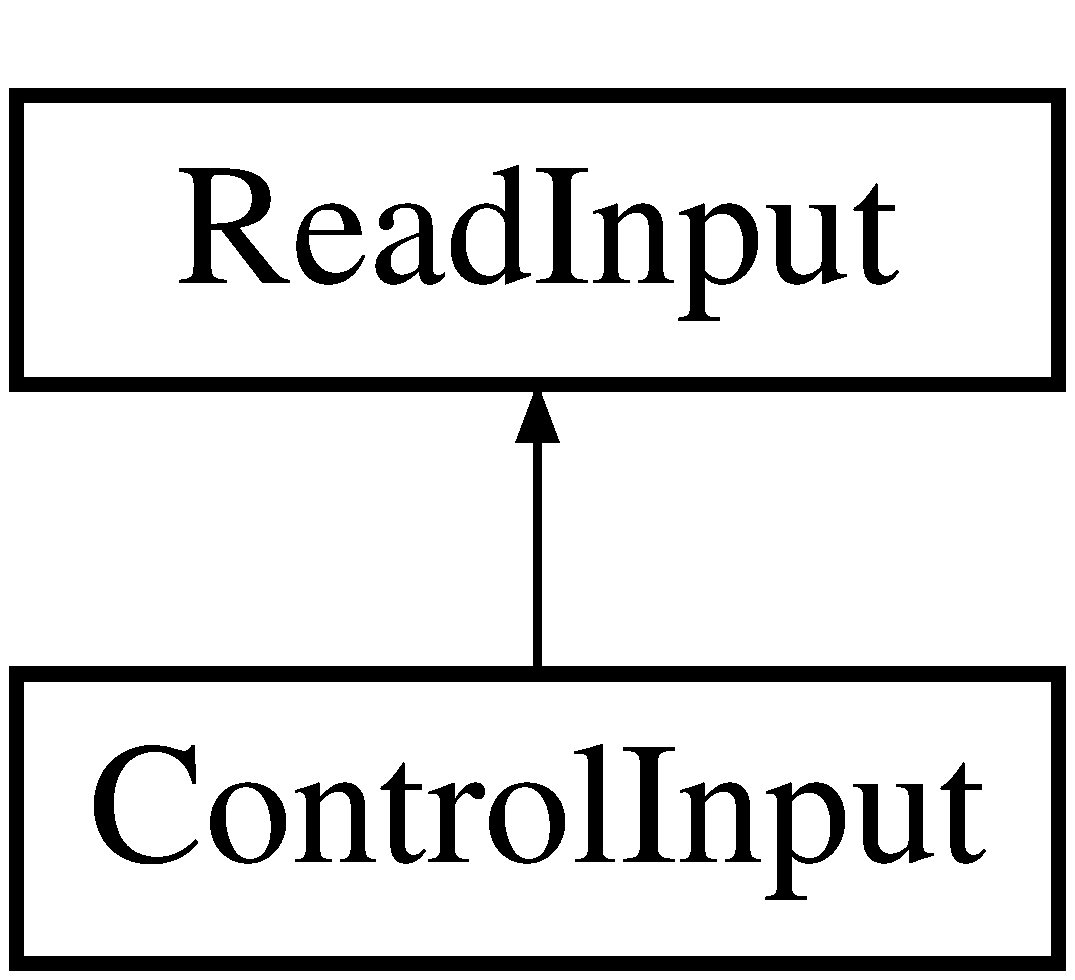
\includegraphics[height=2.000000cm]{class_control_input}
\end{center}
\end{figure}
\subsection*{Public Member Functions}
\begin{DoxyCompactItemize}
\item 
\hyperlink{class_control_input_a50dc4cde4f6410238119971b6934c63a}{Control\-Input} ()
\item 
\hyperlink{class_control_input_aa35022d7c6edbfef7150eb4db594ba58}{$\sim$\-Control\-Input} ()
\item 
void \hyperlink{class_control_input_a2f95d64805ed477f78bf778bb786b30b}{test\-Print} ()
\item 
vector$<$ double $>$ \hyperlink{class_control_input_a3febc929e09306f21f484249c89dbc80}{get\-Wave\-Frequencies} ()
\item 
vector$<$ double $>$ \hyperlink{class_control_input_a2e80de357be6fe5112add0f5066c6328}{get\-Wave\-Directions} ()
\end{DoxyCompactItemize}
\subsection*{Protected Member Functions}
\begin{DoxyCompactItemize}
\item 
void \hyperlink{class_control_input_af15fe8b88a0e7f496c7fd0d4795ff900}{initialize\-Defaults} ()
\item 
int \hyperlink{class_control_input_af7295a9ba455debb812f0e1d4a647820}{legal\-Keyword} (string)
\item 
bool \hyperlink{class_control_input_acb4fb4c1d2a2453e3b8986e44e096f63}{keyword\-Handler} (int, string, string)
\item 
bool \hyperlink{class_control_input_a33b353c2d8f4316d1543059a319faba7}{keyword\-Handler} (int, vector$<$ string $>$, bool)
\end{DoxyCompactItemize}


\subsection{Detailed Description}
This class parses input from file and stores the data appropriately in the \hyperlink{class_system}{System} object. 

\subsection{Constructor \& Destructor Documentation}
\hypertarget{class_control_input_a50dc4cde4f6410238119971b6934c63a}{\index{Control\-Input@{Control\-Input}!Control\-Input@{Control\-Input}}
\index{Control\-Input@{Control\-Input}!ControlInput@{Control\-Input}}
\subsubsection[{Control\-Input}]{\setlength{\rightskip}{0pt plus 5cm}Control\-Input\-::\-Control\-Input (
\begin{DoxyParamCaption}
{}
\end{DoxyParamCaption}
)}}\label{class_control_input_a50dc4cde4f6410238119971b6934c63a}
The default constructor. \hypertarget{class_control_input_aa35022d7c6edbfef7150eb4db594ba58}{\index{Control\-Input@{Control\-Input}!$\sim$\-Control\-Input@{$\sim$\-Control\-Input}}
\index{$\sim$\-Control\-Input@{$\sim$\-Control\-Input}!ControlInput@{Control\-Input}}
\subsubsection[{$\sim$\-Control\-Input}]{\setlength{\rightskip}{0pt plus 5cm}Control\-Input\-::$\sim$\-Control\-Input (
\begin{DoxyParamCaption}
{}
\end{DoxyParamCaption}
)}}\label{class_control_input_aa35022d7c6edbfef7150eb4db594ba58}
The default destructor, nothing happens here. 

\subsection{Member Function Documentation}
\hypertarget{class_control_input_a2e80de357be6fe5112add0f5066c6328}{\index{Control\-Input@{Control\-Input}!get\-Wave\-Directions@{get\-Wave\-Directions}}
\index{get\-Wave\-Directions@{get\-Wave\-Directions}!ControlInput@{Control\-Input}}
\subsubsection[{get\-Wave\-Directions}]{\setlength{\rightskip}{0pt plus 5cm}vector$<$ double $>$ Control\-Input\-::get\-Wave\-Directions (
\begin{DoxyParamCaption}
{}
\end{DoxyParamCaption}
)}}\label{class_control_input_a2e80de357be6fe5112add0f5066c6328}
Get function to retrieve wave directions. \begin{DoxyReturn}{Returns}
the list of wave directions. 
\end{DoxyReturn}
\hypertarget{class_control_input_a3febc929e09306f21f484249c89dbc80}{\index{Control\-Input@{Control\-Input}!get\-Wave\-Frequencies@{get\-Wave\-Frequencies}}
\index{get\-Wave\-Frequencies@{get\-Wave\-Frequencies}!ControlInput@{Control\-Input}}
\subsubsection[{get\-Wave\-Frequencies}]{\setlength{\rightskip}{0pt plus 5cm}vector$<$ double $>$ Control\-Input\-::get\-Wave\-Frequencies (
\begin{DoxyParamCaption}
{}
\end{DoxyParamCaption}
)}}\label{class_control_input_a3febc929e09306f21f484249c89dbc80}
Get function to retrieve wave frequencies. \begin{DoxyReturn}{Returns}
the list of wave frequencies. 
\end{DoxyReturn}
\hypertarget{class_control_input_af15fe8b88a0e7f496c7fd0d4795ff900}{\index{Control\-Input@{Control\-Input}!initialize\-Defaults@{initialize\-Defaults}}
\index{initialize\-Defaults@{initialize\-Defaults}!ControlInput@{Control\-Input}}
\subsubsection[{initialize\-Defaults}]{\setlength{\rightskip}{0pt plus 5cm}void Control\-Input\-::initialize\-Defaults (
\begin{DoxyParamCaption}
{}
\end{DoxyParamCaption}
)\hspace{0.3cm}{\ttfamily [protected]}, {\ttfamily [virtual]}}}\label{class_control_input_af15fe8b88a0e7f496c7fd0d4795ff900}
For future use, does nothing as of now. 

Implements \hyperlink{class_read_input_a4ff2727b876cfd7c01299b08bdd65646}{Read\-Input}.

\hypertarget{class_control_input_acb4fb4c1d2a2453e3b8986e44e096f63}{\index{Control\-Input@{Control\-Input}!keyword\-Handler@{keyword\-Handler}}
\index{keyword\-Handler@{keyword\-Handler}!ControlInput@{Control\-Input}}
\subsubsection[{keyword\-Handler}]{\setlength{\rightskip}{0pt plus 5cm}bool Control\-Input\-::keyword\-Handler (
\begin{DoxyParamCaption}
\item[{int}]{key\-Control, }
\item[{string}]{identifier, }
\item[{string}]{val}
\end{DoxyParamCaption}
)\hspace{0.3cm}{\ttfamily [protected]}, {\ttfamily [virtual]}}}\label{class_control_input_acb4fb4c1d2a2453e3b8986e44e096f63}
Stores the data if valid keyword according to the legeal\-Keyword function. 
\begin{DoxyParams}{Parameters}
{\em key\-Control} & Indicated which case in switch function to use. \\
\hline
{\em identifier} & The keyword. \\
\hline
{\em val} & The value associated with the keyword. \\
\hline
\end{DoxyParams}
\begin{DoxyReturn}{Returns}
false if not done reading data, true to move onto next keyword in parser. 
\end{DoxyReturn}


Implements \hyperlink{class_read_input_a1d8cb0ef59f265300b682de97513f48d}{Read\-Input}.

\hypertarget{class_control_input_a33b353c2d8f4316d1543059a319faba7}{\index{Control\-Input@{Control\-Input}!keyword\-Handler@{keyword\-Handler}}
\index{keyword\-Handler@{keyword\-Handler}!ControlInput@{Control\-Input}}
\subsubsection[{keyword\-Handler}]{\setlength{\rightskip}{0pt plus 5cm}bool Control\-Input\-::keyword\-Handler (
\begin{DoxyParamCaption}
\item[{int}]{key\-Control, }
\item[{vector$<$ string $>$}]{the\-List\-In, }
\item[{bool}]{is\-Direct}
\end{DoxyParamCaption}
)\hspace{0.3cm}{\ttfamily [protected]}, {\ttfamily [virtual]}}}\label{class_control_input_a33b353c2d8f4316d1543059a319faba7}
Stores the list data if valid keyword according to the legeal\-Keyword function. 
\begin{DoxyParams}{Parameters}
{\em key\-Control} & Indicated which case in switch function to use. \\
\hline
{\em the\-List\-In} & List of Values. \\
\hline
{\em is\-Direct} & True if Direct Access List, False if Sequenctial List. \\
\hline
\end{DoxyParams}
\begin{DoxyReturn}{Returns}
false if not done reading data, true to move onto next keyword in parser. 
\end{DoxyReturn}


Implements \hyperlink{class_read_input_afb66a7ff67d0aeb10a3cfa5a4fbc31f8}{Read\-Input}.

\hypertarget{class_control_input_af7295a9ba455debb812f0e1d4a647820}{\index{Control\-Input@{Control\-Input}!legal\-Keyword@{legal\-Keyword}}
\index{legal\-Keyword@{legal\-Keyword}!ControlInput@{Control\-Input}}
\subsubsection[{legal\-Keyword}]{\setlength{\rightskip}{0pt plus 5cm}int Control\-Input\-::legal\-Keyword (
\begin{DoxyParamCaption}
\item[{string}]{string\-In}
\end{DoxyParamCaption}
)\hspace{0.3cm}{\ttfamily [protected]}, {\ttfamily [virtual]}}}\label{class_control_input_af7295a9ba455debb812f0e1d4a647820}
Returns int greater than 0 if the keyword is legal, the int returned specifies how to handle data in keyword\-Handler. 
\begin{DoxyParams}{Parameters}
{\em string\-In} & Check if a valid keyword. \\
\hline
\end{DoxyParams}
\begin{DoxyReturn}{Returns}
int value which tells keyword\-Handler how to handle the data. 
\end{DoxyReturn}


Implements \hyperlink{class_read_input_a4c67f10e813686bf635dd4c6bb2c61bc}{Read\-Input}.

\hypertarget{class_control_input_a2f95d64805ed477f78bf778bb786b30b}{\index{Control\-Input@{Control\-Input}!test\-Print@{test\-Print}}
\index{test\-Print@{test\-Print}!ControlInput@{Control\-Input}}
\subsubsection[{test\-Print}]{\setlength{\rightskip}{0pt plus 5cm}void Control\-Input\-::test\-Print (
\begin{DoxyParamCaption}
{}
\end{DoxyParamCaption}
)}}\label{class_control_input_a2f95d64805ed477f78bf778bb786b30b}
Print to console all data members. 

The documentation for this class was generated from the following files\-:\begin{DoxyCompactItemize}
\item 
Visual Studio 2010/\-Projects/o\-Freq Windows V\-S2010/o\-Freq/controlinput.\-h\item 
Visual Studio 2010/\-Projects/o\-Freq Windows V\-S2010/o\-Freq/controlinput.\-cpp\end{DoxyCompactItemize}

\hypertarget{class_data_input}{\section{Data\-Input Class Reference}
\label{class_data_input}\index{Data\-Input@{Data\-Input}}
}


{\ttfamily \#include $<$datainput.\-h$>$}

Inheritance diagram for Data\-Input\-:\begin{figure}[H]
\begin{center}
\leavevmode
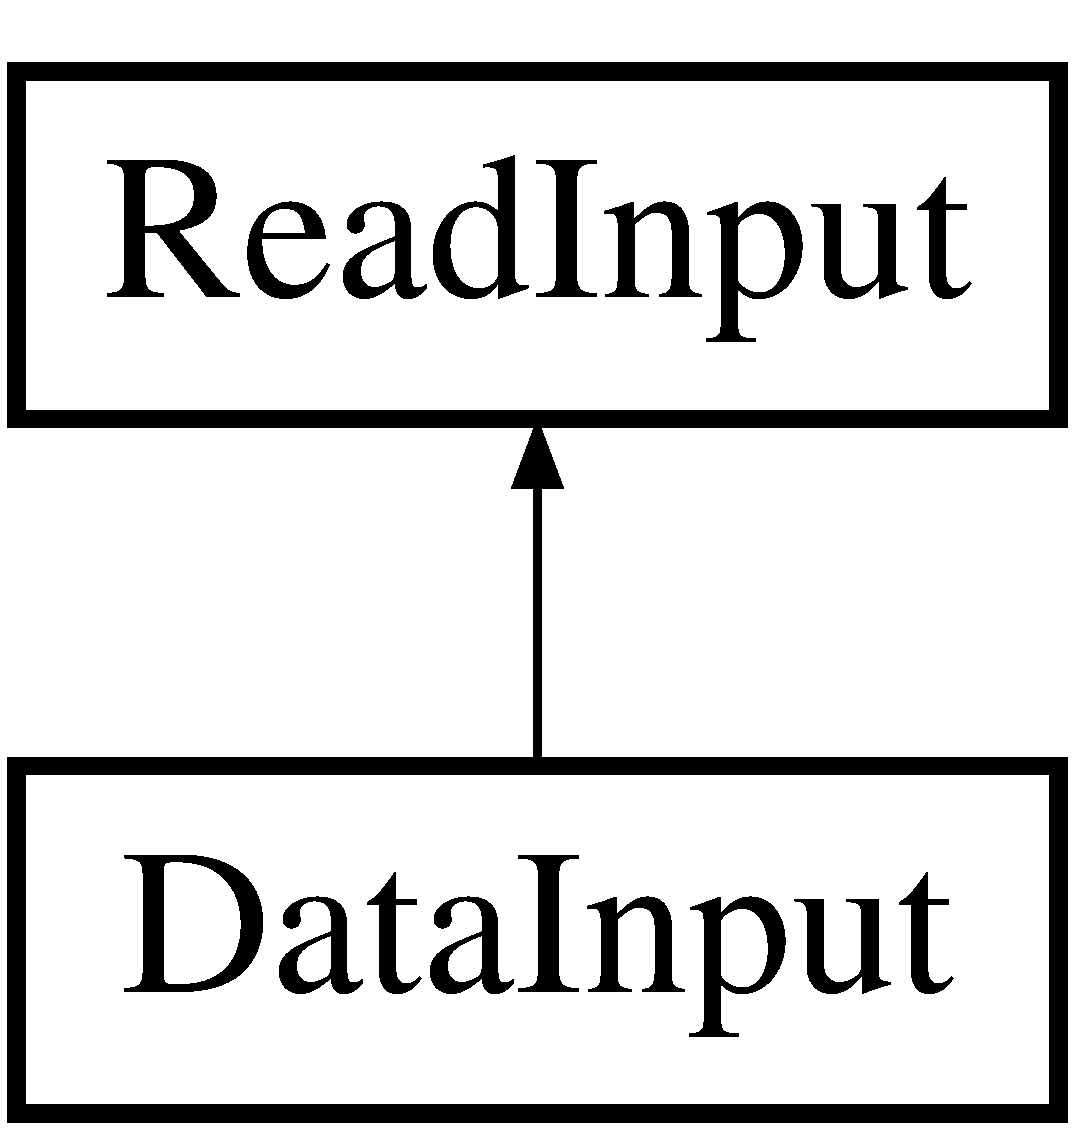
\includegraphics[height=2.000000cm]{class_data_input}
\end{center}
\end{figure}
\subsection*{Public Member Functions}
\begin{DoxyCompactItemize}
\item 
\hyperlink{class_data_input_af2e87fe631ff367c6ef8fa428f3367c4}{Data\-Input} ()
\item 
\hyperlink{class_data_input_a526be3b7b6daeb510ababe0da5222cca}{$\sim$\-Data\-Input} ()
\item 
void \hyperlink{class_data_input_aab1accef9d6147402c2426300656dd3b}{test\-Print} ()
\end{DoxyCompactItemize}
\subsection*{Protected Member Functions}
\begin{DoxyCompactItemize}
\item 
void \hyperlink{class_data_input_a991d4d493aaeaff9d631565b9a49d2ce}{initialize\-Defaults} ()
\item 
int \hyperlink{class_data_input_ae3ca24179103da6e38b99842b9fc1000}{legal\-Keyword} (string)
\item 
bool \hyperlink{class_data_input_a80075c8e86436e00c89d891ce0be57a8}{keyword\-Handler} (int, string, string)
\item 
bool \hyperlink{class_data_input_a70d0380171a30a659a6c7868f2573c92}{keyword\-Handler} (int, vector$<$ string $>$, bool)
\end{DoxyCompactItemize}


\subsection{Detailed Description}
This class parses input from file and stores the data as a list for hyddro file locations. 

\subsection{Constructor \& Destructor Documentation}
\hypertarget{class_data_input_af2e87fe631ff367c6ef8fa428f3367c4}{\index{Data\-Input@{Data\-Input}!Data\-Input@{Data\-Input}}
\index{Data\-Input@{Data\-Input}!DataInput@{Data\-Input}}
\subsubsection[{Data\-Input}]{\setlength{\rightskip}{0pt plus 5cm}Data\-Input\-::\-Data\-Input (
\begin{DoxyParamCaption}
{}
\end{DoxyParamCaption}
)}}\label{class_data_input_af2e87fe631ff367c6ef8fa428f3367c4}
The default constructor. \hypertarget{class_data_input_a526be3b7b6daeb510ababe0da5222cca}{\index{Data\-Input@{Data\-Input}!$\sim$\-Data\-Input@{$\sim$\-Data\-Input}}
\index{$\sim$\-Data\-Input@{$\sim$\-Data\-Input}!DataInput@{Data\-Input}}
\subsubsection[{$\sim$\-Data\-Input}]{\setlength{\rightskip}{0pt plus 5cm}Data\-Input\-::$\sim$\-Data\-Input (
\begin{DoxyParamCaption}
{}
\end{DoxyParamCaption}
)}}\label{class_data_input_a526be3b7b6daeb510ababe0da5222cca}
The default destructor, nothing happens here. 

\subsection{Member Function Documentation}
\hypertarget{class_data_input_a991d4d493aaeaff9d631565b9a49d2ce}{\index{Data\-Input@{Data\-Input}!initialize\-Defaults@{initialize\-Defaults}}
\index{initialize\-Defaults@{initialize\-Defaults}!DataInput@{Data\-Input}}
\subsubsection[{initialize\-Defaults}]{\setlength{\rightskip}{0pt plus 5cm}void Data\-Input\-::initialize\-Defaults (
\begin{DoxyParamCaption}
{}
\end{DoxyParamCaption}
)\hspace{0.3cm}{\ttfamily [protected]}, {\ttfamily [virtual]}}}\label{class_data_input_a991d4d493aaeaff9d631565b9a49d2ce}
For future use, does nothing as of now. 

Implements \hyperlink{class_read_input_a4ff2727b876cfd7c01299b08bdd65646}{Read\-Input}.

\hypertarget{class_data_input_a80075c8e86436e00c89d891ce0be57a8}{\index{Data\-Input@{Data\-Input}!keyword\-Handler@{keyword\-Handler}}
\index{keyword\-Handler@{keyword\-Handler}!DataInput@{Data\-Input}}
\subsubsection[{keyword\-Handler}]{\setlength{\rightskip}{0pt plus 5cm}bool Data\-Input\-::keyword\-Handler (
\begin{DoxyParamCaption}
\item[{int}]{key\-Control, }
\item[{string}]{identifier, }
\item[{string}]{val}
\end{DoxyParamCaption}
)\hspace{0.3cm}{\ttfamily [protected]}, {\ttfamily [virtual]}}}\label{class_data_input_a80075c8e86436e00c89d891ce0be57a8}
Stores the data if valid keyword according to the legeal\-Keyword function. 
\begin{DoxyParams}{Parameters}
{\em key\-Control} & Indicated which case in switch function to use. \\
\hline
{\em identifier} & The keyword. \\
\hline
{\em val} & The value associated with the keyword. \\
\hline
\end{DoxyParams}
\begin{DoxyReturn}{Returns}
false if not done reading data, true to move onto next keyword in parser. 
\end{DoxyReturn}


Implements \hyperlink{class_read_input_a1d8cb0ef59f265300b682de97513f48d}{Read\-Input}.

\hypertarget{class_data_input_a70d0380171a30a659a6c7868f2573c92}{\index{Data\-Input@{Data\-Input}!keyword\-Handler@{keyword\-Handler}}
\index{keyword\-Handler@{keyword\-Handler}!DataInput@{Data\-Input}}
\subsubsection[{keyword\-Handler}]{\setlength{\rightskip}{0pt plus 5cm}bool Data\-Input\-::keyword\-Handler (
\begin{DoxyParamCaption}
\item[{int}]{key\-Control, }
\item[{vector$<$ string $>$}]{the\-List\-In, }
\item[{bool}]{is\-Direct}
\end{DoxyParamCaption}
)\hspace{0.3cm}{\ttfamily [protected]}, {\ttfamily [virtual]}}}\label{class_data_input_a70d0380171a30a659a6c7868f2573c92}
Stores the list data if valid keyword according to the legeal\-Keyword function. 
\begin{DoxyParams}{Parameters}
{\em key\-Control} & Indicated which case in switch function to use. \\
\hline
{\em the\-List\-In} & List of Values. \\
\hline
{\em is\-Direct} & True if Direct Access List, False if Sequenctial List. \\
\hline
\end{DoxyParams}
\begin{DoxyReturn}{Returns}
false if not done reading data, true to move onto next keyword in parser. 
\end{DoxyReturn}


Implements \hyperlink{class_read_input_afb66a7ff67d0aeb10a3cfa5a4fbc31f8}{Read\-Input}.

\hypertarget{class_data_input_ae3ca24179103da6e38b99842b9fc1000}{\index{Data\-Input@{Data\-Input}!legal\-Keyword@{legal\-Keyword}}
\index{legal\-Keyword@{legal\-Keyword}!DataInput@{Data\-Input}}
\subsubsection[{legal\-Keyword}]{\setlength{\rightskip}{0pt plus 5cm}int Data\-Input\-::legal\-Keyword (
\begin{DoxyParamCaption}
\item[{string}]{string\-In}
\end{DoxyParamCaption}
)\hspace{0.3cm}{\ttfamily [protected]}, {\ttfamily [virtual]}}}\label{class_data_input_ae3ca24179103da6e38b99842b9fc1000}
Returns int greater than 0 if the keyword is legal, the int returned specifies how to handle data in keyword\-Handler. 
\begin{DoxyParams}{Parameters}
{\em string\-In} & Check if a valid keyword. \\
\hline
\end{DoxyParams}
\begin{DoxyReturn}{Returns}
int value which tells keyword\-Handler how to handle the data. 
\end{DoxyReturn}


Implements \hyperlink{class_read_input_a4c67f10e813686bf635dd4c6bb2c61bc}{Read\-Input}.

\hypertarget{class_data_input_aab1accef9d6147402c2426300656dd3b}{\index{Data\-Input@{Data\-Input}!test\-Print@{test\-Print}}
\index{test\-Print@{test\-Print}!DataInput@{Data\-Input}}
\subsubsection[{test\-Print}]{\setlength{\rightskip}{0pt plus 5cm}void Data\-Input\-::test\-Print (
\begin{DoxyParamCaption}
{}
\end{DoxyParamCaption}
)}}\label{class_data_input_aab1accef9d6147402c2426300656dd3b}
Print to console all data members. 

The documentation for this class was generated from the following files\-:\begin{DoxyCompactItemize}
\item 
Visual Studio 2010/\-Projects/o\-Freq Windows V\-S2010/o\-Freq/datainput.\-h\item 
Visual Studio 2010/\-Projects/o\-Freq Windows V\-S2010/o\-Freq/datainput.\-cpp\end{DoxyCompactItemize}

\hypertarget{class_derivative}{\section{Derivative Class Reference}
\label{class_derivative}\index{Derivative@{Derivative}}
}


{\ttfamily \#include $<$forcederivative.\-h$>$}

\subsection*{Public Member Functions}
\begin{DoxyCompactItemize}
\item 
\hyperlink{class_derivative_adc03ec3ad150bc0de66a3e7200cd368f}{Derivative} ()
\item 
\hyperlink{class_derivative_a7fc4ee53f460dfb98b3db2e9c9830cf9}{$\sim$\-Derivative} ()
\item 
void \hyperlink{class_derivative_afe00a18765c0d70c3232a41f5ac663dd}{test\-Print} ()
\item 
int \hyperlink{class_derivative_ac95af6fb993314a578b3f0d3cd57a9cc}{get\-Equation\-List\-Size} ()
\end{DoxyCompactItemize}
\subsection*{Public Attributes}
\begin{DoxyCompactItemize}
\item 
\hyperlink{class_equation}{Equation} \hyperlink{class_derivative_a183278e468ffc4d3313968a01c6770ea}{equation\-List} \mbox{[}M\-A\-X\-\_\-\-E\-Q\-U\-A\-T\-I\-O\-N\-S\mbox{]}
\end{DoxyCompactItemize}


\subsection{Detailed Description}
This class holds data for a derivative. 

\subsection{Constructor \& Destructor Documentation}
\hypertarget{class_derivative_adc03ec3ad150bc0de66a3e7200cd368f}{\index{Derivative@{Derivative}!Derivative@{Derivative}}
\index{Derivative@{Derivative}!Derivative@{Derivative}}
\subsubsection[{Derivative}]{\setlength{\rightskip}{0pt plus 5cm}Derivative\-::\-Derivative (
\begin{DoxyParamCaption}
{}
\end{DoxyParamCaption}
)}}\label{class_derivative_adc03ec3ad150bc0de66a3e7200cd368f}
This default constructor creates a \hyperlink{class_body}{Body} object. \hypertarget{class_derivative_a7fc4ee53f460dfb98b3db2e9c9830cf9}{\index{Derivative@{Derivative}!$\sim$\-Derivative@{$\sim$\-Derivative}}
\index{$\sim$\-Derivative@{$\sim$\-Derivative}!Derivative@{Derivative}}
\subsubsection[{$\sim$\-Derivative}]{\setlength{\rightskip}{0pt plus 5cm}Derivative\-::$\sim$\-Derivative (
\begin{DoxyParamCaption}
{}
\end{DoxyParamCaption}
)}}\label{class_derivative_a7fc4ee53f460dfb98b3db2e9c9830cf9}
The default destructor, nothing happens here. 

\subsection{Member Function Documentation}
\hypertarget{class_derivative_ac95af6fb993314a578b3f0d3cd57a9cc}{\index{Derivative@{Derivative}!get\-Equation\-List\-Size@{get\-Equation\-List\-Size}}
\index{get\-Equation\-List\-Size@{get\-Equation\-List\-Size}!Derivative@{Derivative}}
\subsubsection[{get\-Equation\-List\-Size}]{\setlength{\rightskip}{0pt plus 5cm}int Derivative\-::get\-Equation\-List\-Size (
\begin{DoxyParamCaption}
{}
\end{DoxyParamCaption}
)}}\label{class_derivative_ac95af6fb993314a578b3f0d3cd57a9cc}
Retrieve the size of the equation list. \begin{DoxyReturn}{Returns}
The size of the equation list. 
\end{DoxyReturn}
\hypertarget{class_derivative_afe00a18765c0d70c3232a41f5ac663dd}{\index{Derivative@{Derivative}!test\-Print@{test\-Print}}
\index{test\-Print@{test\-Print}!Derivative@{Derivative}}
\subsubsection[{test\-Print}]{\setlength{\rightskip}{0pt plus 5cm}void Derivative\-::test\-Print (
\begin{DoxyParamCaption}
{}
\end{DoxyParamCaption}
)}}\label{class_derivative_afe00a18765c0d70c3232a41f5ac663dd}
Test print to console the values of all data members. 

\subsection{Member Data Documentation}
\hypertarget{class_derivative_a183278e468ffc4d3313968a01c6770ea}{\index{Derivative@{Derivative}!equation\-List@{equation\-List}}
\index{equation\-List@{equation\-List}!Derivative@{Derivative}}
\subsubsection[{equation\-List}]{\setlength{\rightskip}{0pt plus 5cm}{\bf Equation} Derivative\-::equation\-List\mbox{[}M\-A\-X\-\_\-\-E\-Q\-U\-A\-T\-I\-O\-N\-S\mbox{]}}}\label{class_derivative_a183278e468ffc4d3313968a01c6770ea}
The list of equations. 

The documentation for this class was generated from the following files\-:\begin{DoxyCompactItemize}
\item 
Visual Studio 2010/\-Projects/o\-Freq Windows V\-S2010/o\-Freq/forcederivative.\-h\item 
Visual Studio 2010/\-Projects/o\-Freq Windows V\-S2010/o\-Freq/forcederivative.\-cpp\end{DoxyCompactItemize}

\hypertarget{class_equation}{\section{Equation Class Reference}
\label{class_equation}\index{Equation@{Equation}}
}


{\ttfamily \#include $<$forceequation.\-h$>$}

\subsection*{Public Member Functions}
\begin{DoxyCompactItemize}
\item 
\hyperlink{class_equation_a68511fc719250ed80f86c50de9136733}{Equation} ()
\item 
\hyperlink{class_equation_a097243d0dfd608330fc91f115a0d15bb}{$\sim$\-Equation} ()
\item 
void \hyperlink{class_equation_af6c9148998a4abe47f4a4215c51ce3c8}{test\-Print} ()
\item 
int \hyperlink{class_equation_abb01745ac8c816354d72ee529d2bddc0}{get\-Coefficient\-List\-Size} ()
\end{DoxyCompactItemize}
\subsection*{Public Attributes}
\begin{DoxyCompactItemize}
\item 
double \hyperlink{class_equation_a3a17ab6138a657d31dcc9f3e420a0cde}{coefficients} \mbox{[}M\-A\-X\-\_\-\-C\-O\-E\-F\-F\-I\-C\-I\-E\-N\-T\-S\mbox{]}
\end{DoxyCompactItemize}


\subsection{Detailed Description}
This class holds data for an equation. 

\subsection{Constructor \& Destructor Documentation}
\hypertarget{class_equation_a68511fc719250ed80f86c50de9136733}{\index{Equation@{Equation}!Equation@{Equation}}
\index{Equation@{Equation}!Equation@{Equation}}
\subsubsection[{Equation}]{\setlength{\rightskip}{0pt plus 5cm}Equation\-::\-Equation (
\begin{DoxyParamCaption}
{}
\end{DoxyParamCaption}
)}}\label{class_equation_a68511fc719250ed80f86c50de9136733}
This default constructor. \hypertarget{class_equation_a097243d0dfd608330fc91f115a0d15bb}{\index{Equation@{Equation}!$\sim$\-Equation@{$\sim$\-Equation}}
\index{$\sim$\-Equation@{$\sim$\-Equation}!Equation@{Equation}}
\subsubsection[{$\sim$\-Equation}]{\setlength{\rightskip}{0pt plus 5cm}Equation\-::$\sim$\-Equation (
\begin{DoxyParamCaption}
{}
\end{DoxyParamCaption}
)}}\label{class_equation_a097243d0dfd608330fc91f115a0d15bb}
The default destructor, nothing happens here. 

\subsection{Member Function Documentation}
\hypertarget{class_equation_abb01745ac8c816354d72ee529d2bddc0}{\index{Equation@{Equation}!get\-Coefficient\-List\-Size@{get\-Coefficient\-List\-Size}}
\index{get\-Coefficient\-List\-Size@{get\-Coefficient\-List\-Size}!Equation@{Equation}}
\subsubsection[{get\-Coefficient\-List\-Size}]{\setlength{\rightskip}{0pt plus 5cm}int Equation\-::get\-Coefficient\-List\-Size (
\begin{DoxyParamCaption}
{}
\end{DoxyParamCaption}
)}}\label{class_equation_abb01745ac8c816354d72ee529d2bddc0}
Retrieve the size of the coefficient list. \begin{DoxyReturn}{Returns}
The size of the coefficient list. 
\end{DoxyReturn}
\hypertarget{class_equation_af6c9148998a4abe47f4a4215c51ce3c8}{\index{Equation@{Equation}!test\-Print@{test\-Print}}
\index{test\-Print@{test\-Print}!Equation@{Equation}}
\subsubsection[{test\-Print}]{\setlength{\rightskip}{0pt plus 5cm}void Equation\-::test\-Print (
\begin{DoxyParamCaption}
{}
\end{DoxyParamCaption}
)}}\label{class_equation_af6c9148998a4abe47f4a4215c51ce3c8}
Test print to console the values of all data members. 

\subsection{Member Data Documentation}
\hypertarget{class_equation_a3a17ab6138a657d31dcc9f3e420a0cde}{\index{Equation@{Equation}!coefficients@{coefficients}}
\index{coefficients@{coefficients}!Equation@{Equation}}
\subsubsection[{coefficients}]{\setlength{\rightskip}{0pt plus 5cm}double Equation\-::coefficients\mbox{[}M\-A\-X\-\_\-\-C\-O\-E\-F\-F\-I\-C\-I\-E\-N\-T\-S\mbox{]}}}\label{class_equation_a3a17ab6138a657d31dcc9f3e420a0cde}
The list of coeffieints. 

The documentation for this class was generated from the following files\-:\begin{DoxyCompactItemize}
\item 
Visual Studio 2010/\-Projects/o\-Freq Windows V\-S2010/o\-Freq/forceequation.\-h\item 
Visual Studio 2010/\-Projects/o\-Freq Windows V\-S2010/o\-Freq/forceequation.\-cpp\end{DoxyCompactItemize}

\hypertarget{class_equation_of_motion}{\section{Equation\-Of\-Motion Class Reference}
\label{class_equation_of_motion}\index{Equation\-Of\-Motion@{Equation\-Of\-Motion}}
}


{\ttfamily \#include $<$equationofmotion.\-h$>$}

Inheritance diagram for Equation\-Of\-Motion\-:\begin{figure}[H]
\begin{center}
\leavevmode
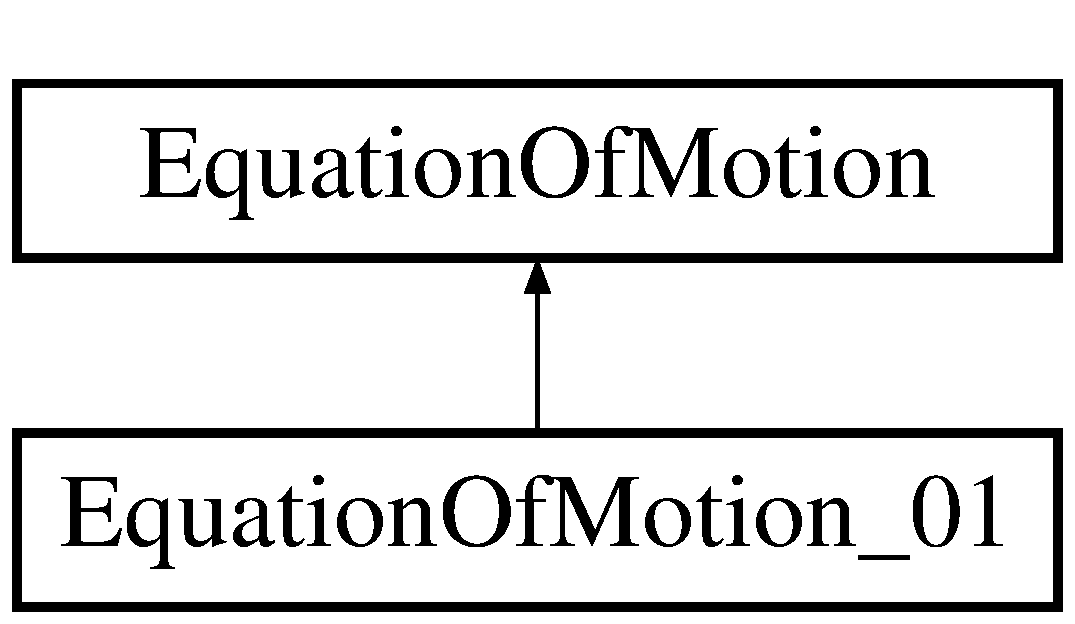
\includegraphics[height=2.000000cm]{class_equation_of_motion}
\end{center}
\end{figure}
\subsection*{Public Member Functions}
\begin{DoxyCompactItemize}
\item 
\hyperlink{class_equation_of_motion_abdb595c57202820b3c78518cb5d459e4}{Equation\-Of\-Motion} ()
\item 
\hyperlink{class_equation_of_motion_ac62caa9b6cdc62ff36d725637e53e62f}{$\sim$\-Equation\-Of\-Motion} ()
\item 
void \hyperlink{class_equation_of_motion_a2c1b3517a0f2aaef687c99fb6b4803dc}{set\-Wave\-Freq} (double)
\item 
virtual void \hyperlink{class_equation_of_motion_a340c67ae539fb20634e7b5bb8edf65f0}{set\-Body\-Data} (\hyperlink{class_body}{Body}, \hyperlink{class_user_forces}{User\-Forces})=0
\item 
\hyperlink{class_body_with_force_matrix}{Body\-With\-Force\-Matrix} \hyperlink{class_equation_of_motion_a7481a809cff3f63523885e1ac372fcc3}{get\-Body\-Force\-Data} ()
\item 
double \hyperlink{class_equation_of_motion_a2b16c339fe40262a4ef1f7b8b0036a01}{kronecker\-Delta} (int, int)
\item 
complex\-Double \hyperlink{class_equation_of_motion_a52e671f290c5a07d1187d56849c84060}{time\-Differentiation} (complex\-Double, int)
\end{DoxyCompactItemize}
\subsection*{Public Attributes}
\begin{DoxyCompactItemize}
\item 
\hyperlink{class_body_with_force_matrix}{Body\-With\-Force\-Matrix} \hyperlink{class_equation_of_motion_aef744ed7692bf6186bb976e0d53f972f}{new\-Body\-Matrix}
\end{DoxyCompactItemize}


\subsection{Detailed Description}
This abstract class holds for data for an equaion of motion. 

\subsection{Constructor \& Destructor Documentation}
\hypertarget{class_equation_of_motion_abdb595c57202820b3c78518cb5d459e4}{\index{Equation\-Of\-Motion@{Equation\-Of\-Motion}!Equation\-Of\-Motion@{Equation\-Of\-Motion}}
\index{Equation\-Of\-Motion@{Equation\-Of\-Motion}!EquationOfMotion@{Equation\-Of\-Motion}}
\subsubsection[{Equation\-Of\-Motion}]{\setlength{\rightskip}{0pt plus 5cm}Equation\-Of\-Motion\-::\-Equation\-Of\-Motion (
\begin{DoxyParamCaption}
{}
\end{DoxyParamCaption}
)}}\label{class_equation_of_motion_abdb595c57202820b3c78518cb5d459e4}
The default constructor. \hypertarget{class_equation_of_motion_ac62caa9b6cdc62ff36d725637e53e62f}{\index{Equation\-Of\-Motion@{Equation\-Of\-Motion}!$\sim$\-Equation\-Of\-Motion@{$\sim$\-Equation\-Of\-Motion}}
\index{$\sim$\-Equation\-Of\-Motion@{$\sim$\-Equation\-Of\-Motion}!EquationOfMotion@{Equation\-Of\-Motion}}
\subsubsection[{$\sim$\-Equation\-Of\-Motion}]{\setlength{\rightskip}{0pt plus 5cm}Equation\-Of\-Motion\-::$\sim$\-Equation\-Of\-Motion (
\begin{DoxyParamCaption}
{}
\end{DoxyParamCaption}
)}}\label{class_equation_of_motion_ac62caa9b6cdc62ff36d725637e53e62f}
The default destructor, nothing happens here. 

\subsection{Member Function Documentation}
\hypertarget{class_equation_of_motion_a7481a809cff3f63523885e1ac372fcc3}{\index{Equation\-Of\-Motion@{Equation\-Of\-Motion}!get\-Body\-Force\-Data@{get\-Body\-Force\-Data}}
\index{get\-Body\-Force\-Data@{get\-Body\-Force\-Data}!EquationOfMotion@{Equation\-Of\-Motion}}
\subsubsection[{get\-Body\-Force\-Data}]{\setlength{\rightskip}{0pt plus 5cm}{\bf Body\-With\-Force\-Matrix} Equation\-Of\-Motion\-::get\-Body\-Force\-Data (
\begin{DoxyParamCaption}
{}
\end{DoxyParamCaption}
)}}\label{class_equation_of_motion_a7481a809cff3f63523885e1ac372fcc3}
Retrieve the body with force matrix object. \begin{DoxyReturn}{Returns}
The body with force matrix object. 
\end{DoxyReturn}
\hypertarget{class_equation_of_motion_a2b16c339fe40262a4ef1f7b8b0036a01}{\index{Equation\-Of\-Motion@{Equation\-Of\-Motion}!kronecker\-Delta@{kronecker\-Delta}}
\index{kronecker\-Delta@{kronecker\-Delta}!EquationOfMotion@{Equation\-Of\-Motion}}
\subsubsection[{kronecker\-Delta}]{\setlength{\rightskip}{0pt plus 5cm}double Equation\-Of\-Motion\-::kronecker\-Delta (
\begin{DoxyParamCaption}
\item[{int}]{num1, }
\item[{int}]{num2}
\end{DoxyParamCaption}
)}}\label{class_equation_of_motion_a2b16c339fe40262a4ef1f7b8b0036a01}
Retrieve the body with force matrix object. 
\begin{DoxyParams}{Parameters}
{\em num1} & An int. \\
\hline
{\em num2} & An int. \\
\hline
\end{DoxyParams}
\begin{DoxyReturn}{Returns}
Return 0 if two numbers are equal or 1 if not. 
\end{DoxyReturn}
\hypertarget{class_equation_of_motion_a340c67ae539fb20634e7b5bb8edf65f0}{\index{Equation\-Of\-Motion@{Equation\-Of\-Motion}!set\-Body\-Data@{set\-Body\-Data}}
\index{set\-Body\-Data@{set\-Body\-Data}!EquationOfMotion@{Equation\-Of\-Motion}}
\subsubsection[{set\-Body\-Data}]{\setlength{\rightskip}{0pt plus 5cm}virtual void Equation\-Of\-Motion\-::set\-Body\-Data (
\begin{DoxyParamCaption}
\item[{{\bf Body}}]{, }
\item[{{\bf User\-Forces}}]{}
\end{DoxyParamCaption}
)\hspace{0.3cm}{\ttfamily [pure virtual]}}}\label{class_equation_of_motion_a340c67ae539fb20634e7b5bb8edf65f0}
This pure virtual function must be implemented by child classes. 
\begin{DoxyParams}{Parameters}
{\em The} & \hyperlink{class_body}{Body}. \\
\hline
{\em The} & User Forces. \\
\hline
\end{DoxyParams}


Implemented in \hyperlink{class_equation_of_motion__01_a97581ef832e495feda5c7f91a30bb8c8}{Equation\-Of\-Motion\-\_\-01}.

\hypertarget{class_equation_of_motion_a2c1b3517a0f2aaef687c99fb6b4803dc}{\index{Equation\-Of\-Motion@{Equation\-Of\-Motion}!set\-Wave\-Freq@{set\-Wave\-Freq}}
\index{set\-Wave\-Freq@{set\-Wave\-Freq}!EquationOfMotion@{Equation\-Of\-Motion}}
\subsubsection[{set\-Wave\-Freq}]{\setlength{\rightskip}{0pt plus 5cm}void Equation\-Of\-Motion\-::set\-Wave\-Freq (
\begin{DoxyParamCaption}
\item[{double}]{new\-Freq\-In}
\end{DoxyParamCaption}
)}}\label{class_equation_of_motion_a2c1b3517a0f2aaef687c99fb6b4803dc}
Sets the current wave frequency to be used. 
\begin{DoxyParams}{Parameters}
{\em new\-Freq\-In} & The current wave frequency. \\
\hline
\end{DoxyParams}
\hypertarget{class_equation_of_motion_a52e671f290c5a07d1187d56849c84060}{\index{Equation\-Of\-Motion@{Equation\-Of\-Motion}!time\-Differentiation@{time\-Differentiation}}
\index{time\-Differentiation@{time\-Differentiation}!EquationOfMotion@{Equation\-Of\-Motion}}
\subsubsection[{time\-Differentiation}]{\setlength{\rightskip}{0pt plus 5cm}complex\-Double Equation\-Of\-Motion\-::time\-Differentiation (
\begin{DoxyParamCaption}
\item[{complex\-Double}]{variable, }
\item[{int}]{order}
\end{DoxyParamCaption}
)}}\label{class_equation_of_motion_a52e671f290c5a07d1187d56849c84060}
Computes the time differention on the values passed in. 
\begin{DoxyParams}{Parameters}
{\em variable} & A force coefficient. \\
\hline
{\em order} & The order derivative. \\
\hline
\end{DoxyParams}
\begin{DoxyReturn}{Returns}
Returns the computed time differentiation. 
\end{DoxyReturn}


\subsection{Member Data Documentation}
\hypertarget{class_equation_of_motion_aef744ed7692bf6186bb976e0d53f972f}{\index{Equation\-Of\-Motion@{Equation\-Of\-Motion}!new\-Body\-Matrix@{new\-Body\-Matrix}}
\index{new\-Body\-Matrix@{new\-Body\-Matrix}!EquationOfMotion@{Equation\-Of\-Motion}}
\subsubsection[{new\-Body\-Matrix}]{\setlength{\rightskip}{0pt plus 5cm}{\bf Body\-With\-Force\-Matrix} Equation\-Of\-Motion\-::new\-Body\-Matrix}}\label{class_equation_of_motion_aef744ed7692bf6186bb976e0d53f972f}
The \hyperlink{class_body}{Body} with force matrix object.. 

The documentation for this class was generated from the following files\-:\begin{DoxyCompactItemize}
\item 
Visual Studio 2010/\-Projects/o\-Freq Windows V\-S2010/o\-Freq/equationofmotion.\-h\item 
Visual Studio 2010/\-Projects/o\-Freq Windows V\-S2010/o\-Freq/equationofmotion.\-cpp\end{DoxyCompactItemize}

\hypertarget{class_equation_of_motion__01}{\section{Equation\-Of\-Motion\-\_\-01 Class Reference}
\label{class_equation_of_motion__01}\index{Equation\-Of\-Motion\-\_\-01@{Equation\-Of\-Motion\-\_\-01}}
}


{\ttfamily \#include $<$equationofmotion\-\_\-01.\-h$>$}

Inheritance diagram for Equation\-Of\-Motion\-\_\-01\-:\begin{figure}[H]
\begin{center}
\leavevmode
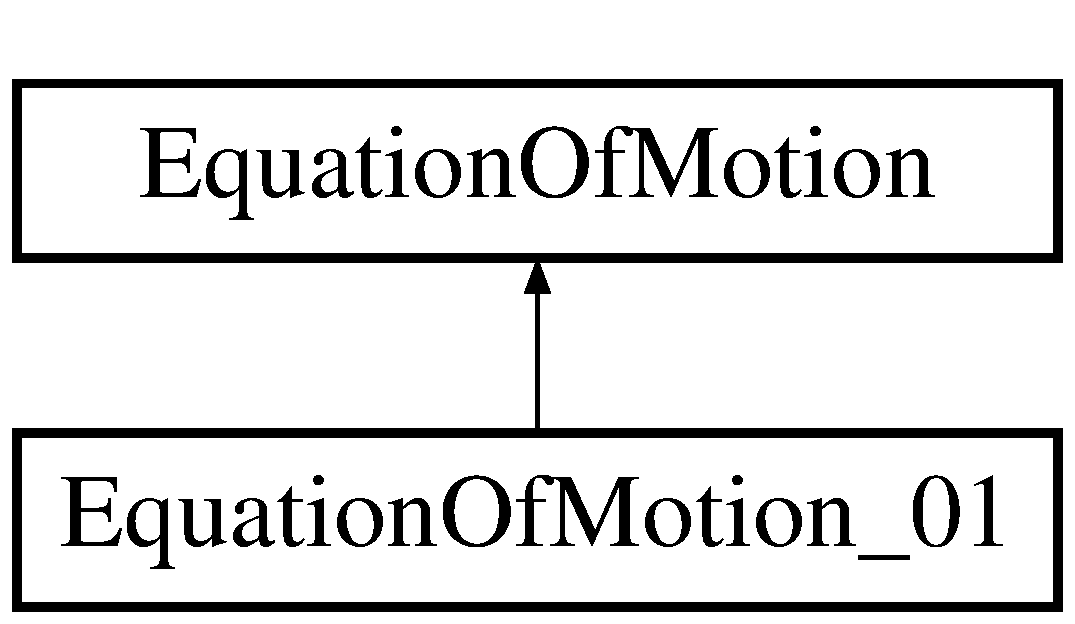
\includegraphics[height=2.000000cm]{class_equation_of_motion__01}
\end{center}
\end{figure}
\subsection*{Public Member Functions}
\begin{DoxyCompactItemize}
\item 
\hyperlink{class_equation_of_motion__01_aeb61f23820f4598eece331449e34643f}{Equation\-Of\-Motion\-\_\-01} ()
\item 
\hyperlink{class_equation_of_motion__01_ae771afba4d9d3b258008493413d0a3a2}{$\sim$\-Equation\-Of\-Motion\-\_\-01} ()
\item 
void \hyperlink{class_equation_of_motion__01_a97581ef832e495feda5c7f91a30bb8c8}{set\-Body\-Data} (\hyperlink{class_body}{Body}, \hyperlink{class_user_forces}{User\-Forces})
\item 
void \hyperlink{class_equation_of_motion__01_a5f38bbfdb6fde4267260216d49b01416}{calculate\-Equations} (\hyperlink{class_body_with_force_matrix}{Body\-With\-Force\-Matrix})
\item 
complex\-Double \hyperlink{class_equation_of_motion__01_a8d21abea0294b0631e5bcbb025a1912d}{get\-Body\-Mass\-Val} (int, int)
\item 
void \hyperlink{class_equation_of_motion__01_a2bd0fd9e562d494c9481f538f7661b1e}{set\-Body\-Mass\-Indexs} (int)
\item 
bool \hyperlink{class_equation_of_motion__01_a69f34f20a208c4b180e24a8aea815fd4}{is\-Current\-Body\-Mass\-Index} (int)
\end{DoxyCompactItemize}
\subsection*{Public Attributes}
\begin{DoxyCompactItemize}
\item 
int \hyperlink{class_equation_of_motion__01_a6f5e508b6824154b02267d7088ec6ba1}{body\-Mass\-Indexs} \mbox{[}body\-Equation\-Size\mbox{]}
\item 
cx\-\_\-mat \hyperlink{class_equation_of_motion__01_a735773656f31e5510aec14d72356801c}{solution\-Matrix}
\end{DoxyCompactItemize}


\subsection{Detailed Description}
This class holds data and functions to calculate the 6\-D\-O\-F \hyperlink{class_equation}{Equation} of Motion. 

\subsection{Constructor \& Destructor Documentation}
\hypertarget{class_equation_of_motion__01_aeb61f23820f4598eece331449e34643f}{\index{Equation\-Of\-Motion\-\_\-01@{Equation\-Of\-Motion\-\_\-01}!Equation\-Of\-Motion\-\_\-01@{Equation\-Of\-Motion\-\_\-01}}
\index{Equation\-Of\-Motion\-\_\-01@{Equation\-Of\-Motion\-\_\-01}!EquationOfMotion_01@{Equation\-Of\-Motion\-\_\-01}}
\subsubsection[{Equation\-Of\-Motion\-\_\-01}]{\setlength{\rightskip}{0pt plus 5cm}Equation\-Of\-Motion\-\_\-01\-::\-Equation\-Of\-Motion\-\_\-01 (
\begin{DoxyParamCaption}
{}
\end{DoxyParamCaption}
)}}\label{class_equation_of_motion__01_aeb61f23820f4598eece331449e34643f}
The default constructor. \hypertarget{class_equation_of_motion__01_ae771afba4d9d3b258008493413d0a3a2}{\index{Equation\-Of\-Motion\-\_\-01@{Equation\-Of\-Motion\-\_\-01}!$\sim$\-Equation\-Of\-Motion\-\_\-01@{$\sim$\-Equation\-Of\-Motion\-\_\-01}}
\index{$\sim$\-Equation\-Of\-Motion\-\_\-01@{$\sim$\-Equation\-Of\-Motion\-\_\-01}!EquationOfMotion_01@{Equation\-Of\-Motion\-\_\-01}}
\subsubsection[{$\sim$\-Equation\-Of\-Motion\-\_\-01}]{\setlength{\rightskip}{0pt plus 5cm}Equation\-Of\-Motion\-\_\-01\-::$\sim$\-Equation\-Of\-Motion\-\_\-01 (
\begin{DoxyParamCaption}
{}
\end{DoxyParamCaption}
)}}\label{class_equation_of_motion__01_ae771afba4d9d3b258008493413d0a3a2}
The default destructor, nothing happens here. 

\subsection{Member Function Documentation}
\hypertarget{class_equation_of_motion__01_a5f38bbfdb6fde4267260216d49b01416}{\index{Equation\-Of\-Motion\-\_\-01@{Equation\-Of\-Motion\-\_\-01}!calculate\-Equations@{calculate\-Equations}}
\index{calculate\-Equations@{calculate\-Equations}!EquationOfMotion_01@{Equation\-Of\-Motion\-\_\-01}}
\subsubsection[{calculate\-Equations}]{\setlength{\rightskip}{0pt plus 5cm}void Equation\-Of\-Motion\-\_\-01\-::calculate\-Equations (
\begin{DoxyParamCaption}
\item[{{\bf Body\-With\-Force\-Matrix}}]{the\-Body\-With\-Force\-Matrices}
\end{DoxyParamCaption}
)}}\label{class_equation_of_motion__01_a5f38bbfdb6fde4267260216d49b01416}
Perform the calculations for the 6\-D\-O\-F Motion Model. 
\begin{DoxyParams}{Parameters}
{\em the\-Body\-With\-Force\-Matrices} & The \hyperlink{class_body}{Body} with force matrices. \\
\hline
\end{DoxyParams}
\hypertarget{class_equation_of_motion__01_a8d21abea0294b0631e5bcbb025a1912d}{\index{Equation\-Of\-Motion\-\_\-01@{Equation\-Of\-Motion\-\_\-01}!get\-Body\-Mass\-Val@{get\-Body\-Mass\-Val}}
\index{get\-Body\-Mass\-Val@{get\-Body\-Mass\-Val}!EquationOfMotion_01@{Equation\-Of\-Motion\-\_\-01}}
\subsubsection[{get\-Body\-Mass\-Val}]{\setlength{\rightskip}{0pt plus 5cm}complex\-Double Equation\-Of\-Motion\-\_\-01\-::get\-Body\-Mass\-Val (
\begin{DoxyParamCaption}
\item[{int}]{equation\-Num, }
\item[{int}]{var}
\end{DoxyParamCaption}
)}}\label{class_equation_of_motion__01_a8d21abea0294b0631e5bcbb025a1912d}
Retrieve a variable in the equaion from the mass matrix. 
\begin{DoxyParams}{Parameters}
{\em equation\-Num} & The equation number (row in mass matrix). \\
\hline
{\em var} & The variable in the equation (column in mass matrix). \\
\hline
\end{DoxyParams}
\begin{DoxyReturn}{Returns}
The variable in the specified equation from the mass matrix. 
\end{DoxyReturn}
\hypertarget{class_equation_of_motion__01_a69f34f20a208c4b180e24a8aea815fd4}{\index{Equation\-Of\-Motion\-\_\-01@{Equation\-Of\-Motion\-\_\-01}!is\-Current\-Body\-Mass\-Index@{is\-Current\-Body\-Mass\-Index}}
\index{is\-Current\-Body\-Mass\-Index@{is\-Current\-Body\-Mass\-Index}!EquationOfMotion_01@{Equation\-Of\-Motion\-\_\-01}}
\subsubsection[{is\-Current\-Body\-Mass\-Index}]{\setlength{\rightskip}{0pt plus 5cm}bool Equation\-Of\-Motion\-\_\-01\-::is\-Current\-Body\-Mass\-Index (
\begin{DoxyParamCaption}
\item[{int}]{cur\-Index}
\end{DoxyParamCaption}
)}}\label{class_equation_of_motion__01_a69f34f20a208c4b180e24a8aea815fd4}
Check if current index is valid in the mass matrix. 
\begin{DoxyParams}{Parameters}
{\em cur\-Index} & The current index in mass matrix. return True if a valid entry in mass matrix. \\
\hline
\end{DoxyParams}
\hypertarget{class_equation_of_motion__01_a97581ef832e495feda5c7f91a30bb8c8}{\index{Equation\-Of\-Motion\-\_\-01@{Equation\-Of\-Motion\-\_\-01}!set\-Body\-Data@{set\-Body\-Data}}
\index{set\-Body\-Data@{set\-Body\-Data}!EquationOfMotion_01@{Equation\-Of\-Motion\-\_\-01}}
\subsubsection[{set\-Body\-Data}]{\setlength{\rightskip}{0pt plus 5cm}void Equation\-Of\-Motion\-\_\-01\-::set\-Body\-Data (
\begin{DoxyParamCaption}
\item[{{\bf Body}}]{body\-Data\-In, }
\item[{{\bf User\-Forces}}]{user\-Forces\-In}
\end{DoxyParamCaption}
)\hspace{0.3cm}{\ttfamily [virtual]}}}\label{class_equation_of_motion__01_a97581ef832e495feda5c7f91a30bb8c8}
Sets the body and forces data for this object. 
\begin{DoxyParams}{Parameters}
{\em body\-Data\-In} & The \hyperlink{class_body}{Body}. \\
\hline
{\em user\-Forces\-In} & The user forces. \\
\hline
\end{DoxyParams}


Implements \hyperlink{class_equation_of_motion_a340c67ae539fb20634e7b5bb8edf65f0}{Equation\-Of\-Motion}.

\hypertarget{class_equation_of_motion__01_a2bd0fd9e562d494c9481f538f7661b1e}{\index{Equation\-Of\-Motion\-\_\-01@{Equation\-Of\-Motion\-\_\-01}!set\-Body\-Mass\-Indexs@{set\-Body\-Mass\-Indexs}}
\index{set\-Body\-Mass\-Indexs@{set\-Body\-Mass\-Indexs}!EquationOfMotion_01@{Equation\-Of\-Motion\-\_\-01}}
\subsubsection[{set\-Body\-Mass\-Indexs}]{\setlength{\rightskip}{0pt plus 5cm}void Equation\-Of\-Motion\-\_\-01\-::set\-Body\-Mass\-Indexs (
\begin{DoxyParamCaption}
\item[{int}]{cur\-Index}
\end{DoxyParamCaption}
)}}\label{class_equation_of_motion__01_a2bd0fd9e562d494c9481f538f7661b1e}
Sets the Indexs in solution matrix, This Needs to be fixed, only supports 2 bodies max. 
\begin{DoxyParams}{Parameters}
{\em cur\-Index} & The current index in the matrix. \\
\hline
\end{DoxyParams}


\subsection{Member Data Documentation}
\hypertarget{class_equation_of_motion__01_a6f5e508b6824154b02267d7088ec6ba1}{\index{Equation\-Of\-Motion\-\_\-01@{Equation\-Of\-Motion\-\_\-01}!body\-Mass\-Indexs@{body\-Mass\-Indexs}}
\index{body\-Mass\-Indexs@{body\-Mass\-Indexs}!EquationOfMotion_01@{Equation\-Of\-Motion\-\_\-01}}
\subsubsection[{body\-Mass\-Indexs}]{\setlength{\rightskip}{0pt plus 5cm}int Equation\-Of\-Motion\-\_\-01\-::body\-Mass\-Indexs\mbox{[}body\-Equation\-Size\mbox{]}}}\label{class_equation_of_motion__01_a6f5e508b6824154b02267d7088ec6ba1}
The indexs in solution matrix for all sub matrices. \hypertarget{class_equation_of_motion__01_a735773656f31e5510aec14d72356801c}{\index{Equation\-Of\-Motion\-\_\-01@{Equation\-Of\-Motion\-\_\-01}!solution\-Matrix@{solution\-Matrix}}
\index{solution\-Matrix@{solution\-Matrix}!EquationOfMotion_01@{Equation\-Of\-Motion\-\_\-01}}
\subsubsection[{solution\-Matrix}]{\setlength{\rightskip}{0pt plus 5cm}cx\-\_\-mat Equation\-Of\-Motion\-\_\-01\-::solution\-Matrix}}\label{class_equation_of_motion__01_a735773656f31e5510aec14d72356801c}
The solution matirx. 

The documentation for this class was generated from the following files\-:\begin{DoxyCompactItemize}
\item 
Visual Studio 2010/\-Projects/o\-Freq Windows V\-S2010/o\-Freq/equationofmotion\-\_\-01.\-h\item 
Visual Studio 2010/\-Projects/o\-Freq Windows V\-S2010/o\-Freq/equationofmotion\-\_\-01.\-cpp\end{DoxyCompactItemize}

\hypertarget{class_file_writer}{\section{File\-Writer Class Reference}
\label{class_file_writer}\index{File\-Writer@{File\-Writer}}
}


{\ttfamily \#include $<$filewriter.\-h$>$}

\subsection*{Public Member Functions}
\begin{DoxyCompactItemize}
\item 
\hyperlink{class_file_writer_a570c654285dedf2eed41794698488268}{File\-Writer} (string, vector$<$ double $>$, vector$<$ double $>$)
\item 
\hyperlink{class_file_writer_ae5490307dcaf9237f4c1b8b8df433e03}{$\sim$\-File\-Writer} ()
\item 
void \hyperlink{class_file_writer_a12fb8cd23937a257e4db0bfade0b2480}{set\-Outputs} (\hyperlink{class_outputs_list}{Outputs\-List})
\item 
bool \hyperlink{class_file_writer_ada65187529c9aceb2be0a66085b745c5}{write\-To\-File} (int)
\item 
bool \hyperlink{class_file_writer_a692853a3380d47586fdc186ca3e62a45}{write\-Directions\-To\-File} (vector$<$ double $>$)
\item 
bool \hyperlink{class_file_writer_a5dd1b1384aac1febb75c21194e43f29e}{write\-Frequencies\-To\-File} (vector$<$ double $>$)
\item 
void \hyperlink{class_file_writer_aeea3ca877f0c5280b22ea7ff653db233}{set\-Header} ()
\item 
void \hyperlink{class_file_writer_aa01e35cc83c9ddee419c2b08cf12e919}{set\-File\-Info} (string)
\item 
bool \hyperlink{class_file_writer_a3c651fa84b2cce465f2ec0fce8be2464}{remove\-Old\-Directories} ()
\end{DoxyCompactItemize}


\subsection{Detailed Description}
This class write all outputs to files. 

\subsection{Constructor \& Destructor Documentation}
\hypertarget{class_file_writer_a570c654285dedf2eed41794698488268}{\index{File\-Writer@{File\-Writer}!File\-Writer@{File\-Writer}}
\index{File\-Writer@{File\-Writer}!FileWriter@{File\-Writer}}
\subsubsection[{File\-Writer}]{\setlength{\rightskip}{0pt plus 5cm}File\-Writer\-::\-File\-Writer (
\begin{DoxyParamCaption}
\item[{string}]{file\-Dir\-In, }
\item[{vector$<$ double $>$}]{the\-Directions\-List\-In, }
\item[{vector$<$ double $>$}]{the\-Frequencies\-List\-In}
\end{DoxyParamCaption}
)}}\label{class_file_writer_a570c654285dedf2eed41794698488268}
Constructor on creation sets header, write wave directions \& frequencies to file, and removes old directories 
\begin{DoxyParams}{Parameters}
{\em file\-Dir\-In} & The directory to write outputs. \\
\hline
{\em the\-Directions\-List\-In} & The list of wave directions. \\
\hline
{\em the\-Frequencies\-List\-In} & The list of wave frequncies \\
\hline
\end{DoxyParams}
\hypertarget{class_file_writer_ae5490307dcaf9237f4c1b8b8df433e03}{\index{File\-Writer@{File\-Writer}!$\sim$\-File\-Writer@{$\sim$\-File\-Writer}}
\index{$\sim$\-File\-Writer@{$\sim$\-File\-Writer}!FileWriter@{File\-Writer}}
\subsubsection[{$\sim$\-File\-Writer}]{\setlength{\rightskip}{0pt plus 5cm}File\-Writer\-::$\sim$\-File\-Writer (
\begin{DoxyParamCaption}
{}
\end{DoxyParamCaption}
)}}\label{class_file_writer_ae5490307dcaf9237f4c1b8b8df433e03}
The default destructor, nothing happens here. 

\subsection{Member Function Documentation}
\hypertarget{class_file_writer_a3c651fa84b2cce465f2ec0fce8be2464}{\index{File\-Writer@{File\-Writer}!remove\-Old\-Directories@{remove\-Old\-Directories}}
\index{remove\-Old\-Directories@{remove\-Old\-Directories}!FileWriter@{File\-Writer}}
\subsubsection[{remove\-Old\-Directories}]{\setlength{\rightskip}{0pt plus 5cm}bool File\-Writer\-::remove\-Old\-Directories (
\begin{DoxyParamCaption}
{}
\end{DoxyParamCaption}
)}}\label{class_file_writer_a3c651fa84b2cce465f2ec0fce8be2464}
Remove all old directiories \& files written by o\-Freq previous run. \begin{DoxyReturn}{Returns}
Return true if all files \& directories were successfully deleted. 
\end{DoxyReturn}
\hypertarget{class_file_writer_aa01e35cc83c9ddee419c2b08cf12e919}{\index{File\-Writer@{File\-Writer}!set\-File\-Info@{set\-File\-Info}}
\index{set\-File\-Info@{set\-File\-Info}!FileWriter@{File\-Writer}}
\subsubsection[{set\-File\-Info}]{\setlength{\rightskip}{0pt plus 5cm}void File\-Writer\-::set\-File\-Info (
\begin{DoxyParamCaption}
\item[{string}]{object\-In}
\end{DoxyParamCaption}
)}}\label{class_file_writer_aa01e35cc83c9ddee419c2b08cf12e919}
Set information about the file to be written after header and above data, included in the seafile block. 
\begin{DoxyParams}{Parameters}
{\em object\-In} & The name of the object. \\
\hline
\end{DoxyParams}
\hypertarget{class_file_writer_aeea3ca877f0c5280b22ea7ff653db233}{\index{File\-Writer@{File\-Writer}!set\-Header@{set\-Header}}
\index{set\-Header@{set\-Header}!FileWriter@{File\-Writer}}
\subsubsection[{set\-Header}]{\setlength{\rightskip}{0pt plus 5cm}void File\-Writer\-::set\-Header (
\begin{DoxyParamCaption}
{}
\end{DoxyParamCaption}
)}}\label{class_file_writer_aeea3ca877f0c5280b22ea7ff653db233}
Reads in from input file the header to be used in all files. \hypertarget{class_file_writer_a12fb8cd23937a257e4db0bfade0b2480}{\index{File\-Writer@{File\-Writer}!set\-Outputs@{set\-Outputs}}
\index{set\-Outputs@{set\-Outputs}!FileWriter@{File\-Writer}}
\subsubsection[{set\-Outputs}]{\setlength{\rightskip}{0pt plus 5cm}void File\-Writer\-::set\-Outputs (
\begin{DoxyParamCaption}
\item[{{\bf Outputs\-List}}]{the\-Outputs\-List\-In}
\end{DoxyParamCaption}
)}}\label{class_file_writer_a12fb8cd23937a257e4db0bfade0b2480}
Sets the outputs that will be written to file later. 
\begin{DoxyParams}{Parameters}
{\em the\-Outputs\-List\-In} & The list of outputs. \\
\hline
\end{DoxyParams}
\hypertarget{class_file_writer_a692853a3380d47586fdc186ca3e62a45}{\index{File\-Writer@{File\-Writer}!write\-Directions\-To\-File@{write\-Directions\-To\-File}}
\index{write\-Directions\-To\-File@{write\-Directions\-To\-File}!FileWriter@{File\-Writer}}
\subsubsection[{write\-Directions\-To\-File}]{\setlength{\rightskip}{0pt plus 5cm}bool File\-Writer\-::write\-Directions\-To\-File (
\begin{DoxyParamCaption}
\item[{vector$<$ double $>$}]{direction\-List}
\end{DoxyParamCaption}
)}}\label{class_file_writer_a692853a3380d47586fdc186ca3e62a45}
Writes the directions list to file. 
\begin{DoxyParams}{Parameters}
{\em direction\-List} & The list of directions. \\
\hline
\end{DoxyParams}
\begin{DoxyReturn}{Returns}
true if write successful. 
\end{DoxyReturn}
\hypertarget{class_file_writer_a5dd1b1384aac1febb75c21194e43f29e}{\index{File\-Writer@{File\-Writer}!write\-Frequencies\-To\-File@{write\-Frequencies\-To\-File}}
\index{write\-Frequencies\-To\-File@{write\-Frequencies\-To\-File}!FileWriter@{File\-Writer}}
\subsubsection[{write\-Frequencies\-To\-File}]{\setlength{\rightskip}{0pt plus 5cm}bool File\-Writer\-::write\-Frequencies\-To\-File (
\begin{DoxyParamCaption}
\item[{vector$<$ double $>$}]{frequency\-List}
\end{DoxyParamCaption}
)}}\label{class_file_writer_a5dd1b1384aac1febb75c21194e43f29e}
Writes the frequencies list to file. 
\begin{DoxyParams}{Parameters}
{\em frequency\-List} & The list of frequencies. \\
\hline
\end{DoxyParams}
\begin{DoxyReturn}{Returns}
true if write successful. 
\end{DoxyReturn}
\hypertarget{class_file_writer_ada65187529c9aceb2be0a66085b745c5}{\index{File\-Writer@{File\-Writer}!write\-To\-File@{write\-To\-File}}
\index{write\-To\-File@{write\-To\-File}!FileWriter@{File\-Writer}}
\subsubsection[{write\-To\-File}]{\setlength{\rightskip}{0pt plus 5cm}bool File\-Writer\-::write\-To\-File (
\begin{DoxyParamCaption}
\item[{int}]{cur\-Wave\-Direction}
\end{DoxyParamCaption}
)}}\label{class_file_writer_ada65187529c9aceb2be0a66085b745c5}
Writes the outputs list to file. 
\begin{DoxyParams}{Parameters}
{\em cur\-Wave\-Direction} & The current wave direction. \\
\hline
\end{DoxyParams}
\begin{DoxyReturn}{Returns}
true if write successful. 
\end{DoxyReturn}


The documentation for this class was generated from the following files\-:\begin{DoxyCompactItemize}
\item 
Visual Studio 2010/\-Projects/o\-Freq Windows V\-S2010/o\-Freq/filewriter.\-h\item 
Visual Studio 2010/\-Projects/o\-Freq Windows V\-S2010/o\-Freq/filewriter.\-cpp\end{DoxyCompactItemize}

\hypertarget{class_force}{\section{Force Class Reference}
\label{class_force}\index{Force@{Force}}
}


{\ttfamily \#include $<$force.\-h$>$}

Inheritance diagram for Force\-:\begin{figure}[H]
\begin{center}
\leavevmode
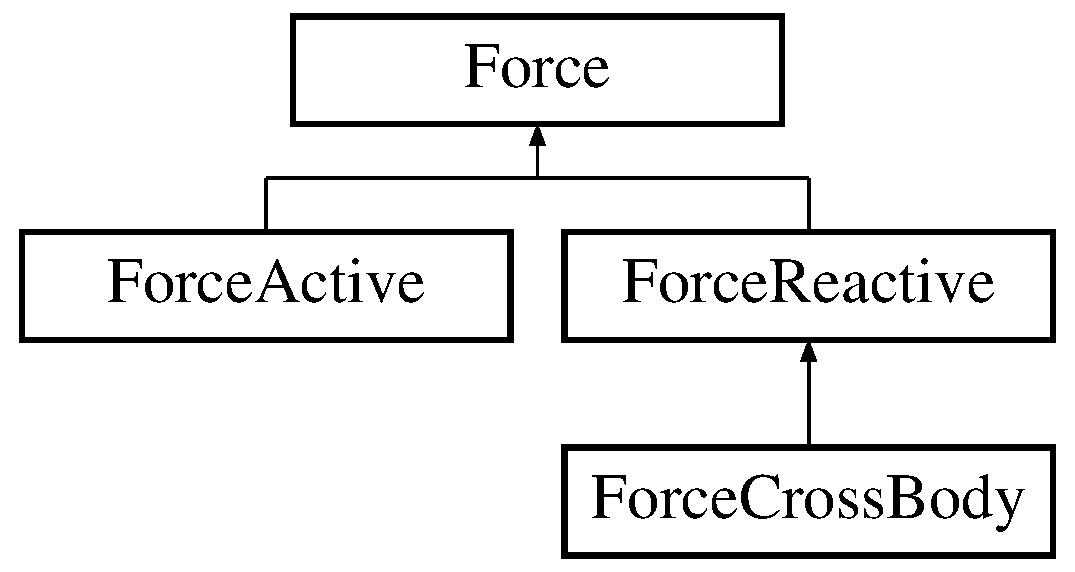
\includegraphics[height=3.000000cm]{class_force}
\end{center}
\end{figure}
\subsection*{Public Member Functions}
\begin{DoxyCompactItemize}
\item 
\hyperlink{class_force_a00983e3bbc206a00bb9253deafc4e424}{Force} ()
\item 
\hyperlink{class_force_a8767ca332cee738a462befe1bfbfa454}{$\sim$\-Force} ()
\item 
void \hyperlink{class_force_aefb0b71694f6ffbfe1ee06516f5536c3}{set\-Force\-Name} (string)
\item 
string \hyperlink{class_force_a8431fcc0edd27e3edb77f8176bec6908}{get\-Force\-Name} ()
\end{DoxyCompactItemize}
\subsection*{Protected Attributes}
\begin{DoxyCompactItemize}
\item 
string \hyperlink{class_force_a50b8739b17f549bd250936b0251ca571}{force\-Name}
\end{DoxyCompactItemize}


\subsection{Detailed Description}
This (base) class holds data for a force object. 

\subsection{Constructor \& Destructor Documentation}
\hypertarget{class_force_a00983e3bbc206a00bb9253deafc4e424}{\index{Force@{Force}!Force@{Force}}
\index{Force@{Force}!Force@{Force}}
\subsubsection[{Force}]{\setlength{\rightskip}{0pt plus 5cm}Force\-::\-Force (
\begin{DoxyParamCaption}
{}
\end{DoxyParamCaption}
)}}\label{class_force_a00983e3bbc206a00bb9253deafc4e424}
The default constructor. \hypertarget{class_force_a8767ca332cee738a462befe1bfbfa454}{\index{Force@{Force}!$\sim$\-Force@{$\sim$\-Force}}
\index{$\sim$\-Force@{$\sim$\-Force}!Force@{Force}}
\subsubsection[{$\sim$\-Force}]{\setlength{\rightskip}{0pt plus 5cm}Force\-::$\sim$\-Force (
\begin{DoxyParamCaption}
{}
\end{DoxyParamCaption}
)}}\label{class_force_a8767ca332cee738a462befe1bfbfa454}
The default destructor, nothing happens here. 

\subsection{Member Function Documentation}
\hypertarget{class_force_a8431fcc0edd27e3edb77f8176bec6908}{\index{Force@{Force}!get\-Force\-Name@{get\-Force\-Name}}
\index{get\-Force\-Name@{get\-Force\-Name}!Force@{Force}}
\subsubsection[{get\-Force\-Name}]{\setlength{\rightskip}{0pt plus 5cm}string Force\-::get\-Force\-Name (
\begin{DoxyParamCaption}
{}
\end{DoxyParamCaption}
)}}\label{class_force_a8431fcc0edd27e3edb77f8176bec6908}
Retrieve the name of the force. \begin{DoxyReturn}{Returns}
new\-Name The name of the force. 
\end{DoxyReturn}
\hypertarget{class_force_aefb0b71694f6ffbfe1ee06516f5536c3}{\index{Force@{Force}!set\-Force\-Name@{set\-Force\-Name}}
\index{set\-Force\-Name@{set\-Force\-Name}!Force@{Force}}
\subsubsection[{set\-Force\-Name}]{\setlength{\rightskip}{0pt plus 5cm}void Force\-::set\-Force\-Name (
\begin{DoxyParamCaption}
\item[{string}]{new\-Name}
\end{DoxyParamCaption}
)}}\label{class_force_aefb0b71694f6ffbfe1ee06516f5536c3}
Sets the name of the force. 
\begin{DoxyParams}{Parameters}
{\em new\-Name} & The name of the force. \\
\hline
\end{DoxyParams}


\subsection{Member Data Documentation}
\hypertarget{class_force_a50b8739b17f549bd250936b0251ca571}{\index{Force@{Force}!force\-Name@{force\-Name}}
\index{force\-Name@{force\-Name}!Force@{Force}}
\subsubsection[{force\-Name}]{\setlength{\rightskip}{0pt plus 5cm}string Force\-::force\-Name\hspace{0.3cm}{\ttfamily [protected]}}}\label{class_force_a50b8739b17f549bd250936b0251ca571}
The force name. 

The documentation for this class was generated from the following files\-:\begin{DoxyCompactItemize}
\item 
Visual Studio 2010/\-Projects/o\-Freq Windows V\-S2010/o\-Freq/force.\-h\item 
Visual Studio 2010/\-Projects/o\-Freq Windows V\-S2010/o\-Freq/force.\-cpp\end{DoxyCompactItemize}

\hypertarget{class_force_active}{\section{Force\-Active Class Reference}
\label{class_force_active}\index{Force\-Active@{Force\-Active}}
}


{\ttfamily \#include $<$forceactive.\-h$>$}

Inheritance diagram for Force\-Active\-:\begin{figure}[H]
\begin{center}
\leavevmode
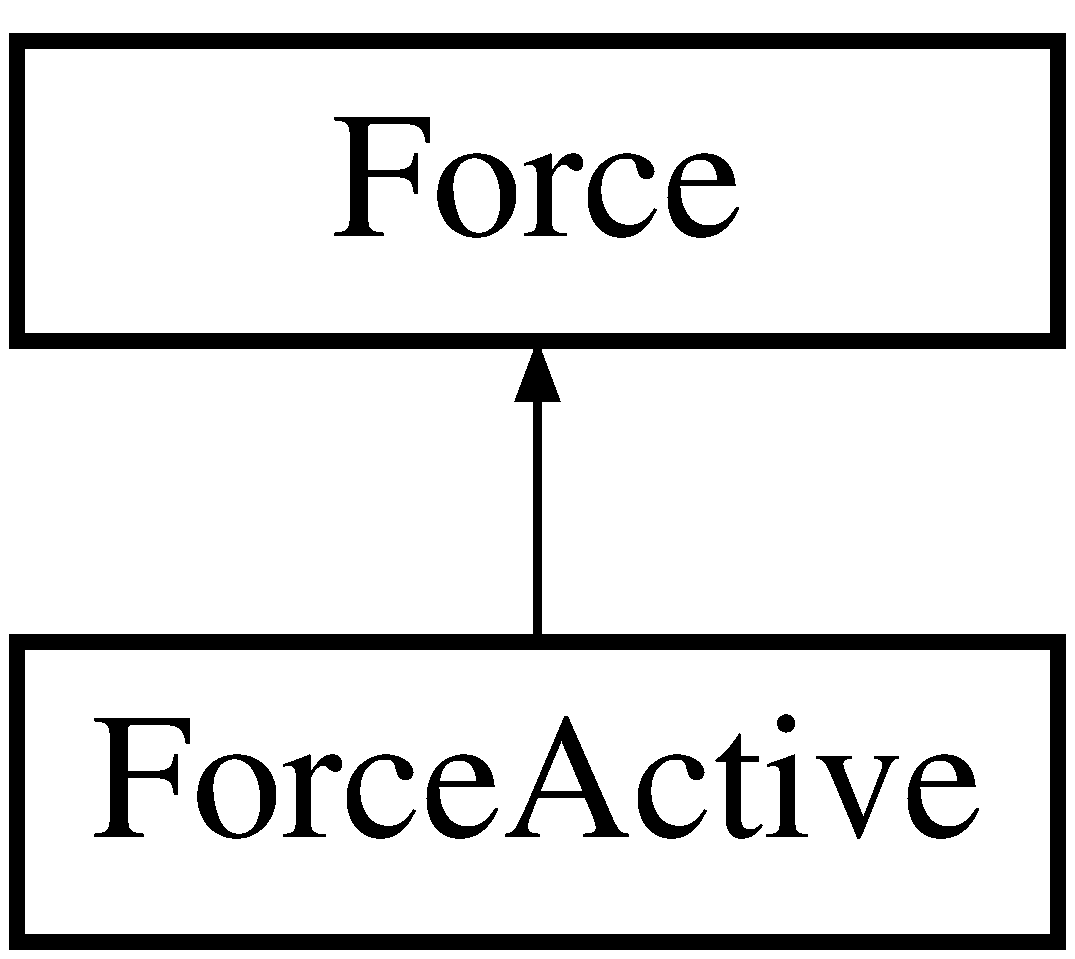
\includegraphics[height=2.000000cm]{class_force_active}
\end{center}
\end{figure}
\subsection*{Public Member Functions}
\begin{DoxyCompactItemize}
\item 
\hyperlink{class_force_active_ae006e3394f8c925c6a3218686c5cc8ae}{Force\-Active} ()
\item 
\hyperlink{class_force_active_aa2db4bc1fb74ecb6e0ee46c59a40dd2a}{$\sim$\-Force\-Active} ()
\item 
void \hyperlink{class_force_active_a8f209e7485e2086c4b7013511a96961e}{test\-Print} ()
\item 
complex\-Double \hyperlink{class_force_active_aebc48c0ba0f2d7a2a18059ad7ff1c3e8}{convert\-Rectangular\-Form\-To\-Complex\-Number} (string)
\item 
complex\-Double \hyperlink{class_force_active_a3e8d5604c7e0ecf12fbe1d1acf1a2e89}{convert\-Polar\-Form\-To\-Complex\-Number} (string)
\item 
void \hyperlink{class_force_active_a54690a658cdb9d7684f3063420ec6e1c}{set\-Coeff} (vector$<$ string $>$, bool)
\item 
vector$<$ complex\-Double $>$ \hyperlink{class_force_active_a9a4b712b31f3c40327a6bb68ff1aa565}{get\-Coefficients} ()
\end{DoxyCompactItemize}
\subsection*{Protected Attributes}
\begin{DoxyCompactItemize}
\item 
complex\-Double \hyperlink{class_force_active_ab83eebfa9ec47878caa32da3f8885022}{coefficients} \mbox{[}M\-A\-X\-\_\-\-C\-O\-E\-F\-F\-I\-C\-I\-E\-N\-T\-S\mbox{]}
\end{DoxyCompactItemize}


\subsection{Detailed Description}
This class holds data for an active force. 

\subsection{Constructor \& Destructor Documentation}
\hypertarget{class_force_active_ae006e3394f8c925c6a3218686c5cc8ae}{\index{Force\-Active@{Force\-Active}!Force\-Active@{Force\-Active}}
\index{Force\-Active@{Force\-Active}!ForceActive@{Force\-Active}}
\subsubsection[{Force\-Active}]{\setlength{\rightskip}{0pt plus 5cm}Force\-Active\-::\-Force\-Active (
\begin{DoxyParamCaption}
{}
\end{DoxyParamCaption}
)}}\label{class_force_active_ae006e3394f8c925c6a3218686c5cc8ae}
The default constructor. \hypertarget{class_force_active_aa2db4bc1fb74ecb6e0ee46c59a40dd2a}{\index{Force\-Active@{Force\-Active}!$\sim$\-Force\-Active@{$\sim$\-Force\-Active}}
\index{$\sim$\-Force\-Active@{$\sim$\-Force\-Active}!ForceActive@{Force\-Active}}
\subsubsection[{$\sim$\-Force\-Active}]{\setlength{\rightskip}{0pt plus 5cm}Force\-Active\-::$\sim$\-Force\-Active (
\begin{DoxyParamCaption}
{}
\end{DoxyParamCaption}
)}}\label{class_force_active_aa2db4bc1fb74ecb6e0ee46c59a40dd2a}
The default destructor, nothing happens here. 

\subsection{Member Function Documentation}
\hypertarget{class_force_active_a3e8d5604c7e0ecf12fbe1d1acf1a2e89}{\index{Force\-Active@{Force\-Active}!convert\-Polar\-Form\-To\-Complex\-Number@{convert\-Polar\-Form\-To\-Complex\-Number}}
\index{convert\-Polar\-Form\-To\-Complex\-Number@{convert\-Polar\-Form\-To\-Complex\-Number}!ForceActive@{Force\-Active}}
\subsubsection[{convert\-Polar\-Form\-To\-Complex\-Number}]{\setlength{\rightskip}{0pt plus 5cm}complex\-Double Force\-Active\-::convert\-Polar\-Form\-To\-Complex\-Number (
\begin{DoxyParamCaption}
\item[{string}]{expression}
\end{DoxyParamCaption}
)}}\label{class_force_active_a3e8d5604c7e0ecf12fbe1d1acf1a2e89}
Converts string in polar form to a complex number. 
\begin{DoxyParams}{Parameters}
{\em expression} & The string in polar form. \\
\hline
\end{DoxyParams}
\begin{DoxyReturn}{Returns}
a complex number. 
\end{DoxyReturn}
\hypertarget{class_force_active_aebc48c0ba0f2d7a2a18059ad7ff1c3e8}{\index{Force\-Active@{Force\-Active}!convert\-Rectangular\-Form\-To\-Complex\-Number@{convert\-Rectangular\-Form\-To\-Complex\-Number}}
\index{convert\-Rectangular\-Form\-To\-Complex\-Number@{convert\-Rectangular\-Form\-To\-Complex\-Number}!ForceActive@{Force\-Active}}
\subsubsection[{convert\-Rectangular\-Form\-To\-Complex\-Number}]{\setlength{\rightskip}{0pt plus 5cm}complex\-Double Force\-Active\-::convert\-Rectangular\-Form\-To\-Complex\-Number (
\begin{DoxyParamCaption}
\item[{string}]{expression}
\end{DoxyParamCaption}
)}}\label{class_force_active_aebc48c0ba0f2d7a2a18059ad7ff1c3e8}
Converts string in rectanguluar form to a complex number. 
\begin{DoxyParams}{Parameters}
{\em expression} & The string in Rectanguluar form. \\
\hline
\end{DoxyParams}
\begin{DoxyReturn}{Returns}
a complex number. 
\end{DoxyReturn}
\hypertarget{class_force_active_a9a4b712b31f3c40327a6bb68ff1aa565}{\index{Force\-Active@{Force\-Active}!get\-Coefficients@{get\-Coefficients}}
\index{get\-Coefficients@{get\-Coefficients}!ForceActive@{Force\-Active}}
\subsubsection[{get\-Coefficients}]{\setlength{\rightskip}{0pt plus 5cm}vector$<$ complex\-Double $>$ Force\-Active\-::get\-Coefficients (
\begin{DoxyParamCaption}
{}
\end{DoxyParamCaption}
)}}\label{class_force_active_a9a4b712b31f3c40327a6bb68ff1aa565}
Retrieve the list of coefficients. \begin{DoxyReturn}{Returns}
The list of coefficients. 
\end{DoxyReturn}
\hypertarget{class_force_active_a54690a658cdb9d7684f3063420ec6e1c}{\index{Force\-Active@{Force\-Active}!set\-Coeff@{set\-Coeff}}
\index{set\-Coeff@{set\-Coeff}!ForceActive@{Force\-Active}}
\subsubsection[{set\-Coeff}]{\setlength{\rightskip}{0pt plus 5cm}void Force\-Active\-::set\-Coeff (
\begin{DoxyParamCaption}
\item[{vector$<$ string $>$}]{the\-List\-In, }
\item[{bool}]{is\-Direct\-List}
\end{DoxyParamCaption}
)}}\label{class_force_active_a54690a658cdb9d7684f3063420ec6e1c}
Set the coefficients. 
\begin{DoxyParams}{Parameters}
{\em the\-List\-In} & The list of coefficients. \\
\hline
{\em is\-Direct\-List} & Specifies whether list of coefficients is direct list or sequential list. \\
\hline
\end{DoxyParams}
\hypertarget{class_force_active_a8f209e7485e2086c4b7013511a96961e}{\index{Force\-Active@{Force\-Active}!test\-Print@{test\-Print}}
\index{test\-Print@{test\-Print}!ForceActive@{Force\-Active}}
\subsubsection[{test\-Print}]{\setlength{\rightskip}{0pt plus 5cm}void Force\-Active\-::test\-Print (
\begin{DoxyParamCaption}
{}
\end{DoxyParamCaption}
)}}\label{class_force_active_a8f209e7485e2086c4b7013511a96961e}
Test print to console the values of all data members. 

\subsection{Member Data Documentation}
\hypertarget{class_force_active_ab83eebfa9ec47878caa32da3f8885022}{\index{Force\-Active@{Force\-Active}!coefficients@{coefficients}}
\index{coefficients@{coefficients}!ForceActive@{Force\-Active}}
\subsubsection[{coefficients}]{\setlength{\rightskip}{0pt plus 5cm}complex\-Double Force\-Active\-::coefficients\mbox{[}M\-A\-X\-\_\-\-C\-O\-E\-F\-F\-I\-C\-I\-E\-N\-T\-S\mbox{]}\hspace{0.3cm}{\ttfamily [protected]}}}\label{class_force_active_ab83eebfa9ec47878caa32da3f8885022}
The list of force coeffients. 

The documentation for this class was generated from the following files\-:\begin{DoxyCompactItemize}
\item 
Visual Studio 2010/\-Projects/o\-Freq Windows V\-S2010/o\-Freq/forceactive.\-h\item 
Visual Studio 2010/\-Projects/o\-Freq Windows V\-S2010/o\-Freq/forceactive.\-cpp\end{DoxyCompactItemize}

\hypertarget{class_force_cross_body}{\section{Force\-Cross\-Body Class Reference}
\label{class_force_cross_body}\index{Force\-Cross\-Body@{Force\-Cross\-Body}}
}


{\ttfamily \#include $<$forcecrossbody.\-h$>$}

Inheritance diagram for Force\-Cross\-Body\-:\begin{figure}[H]
\begin{center}
\leavevmode
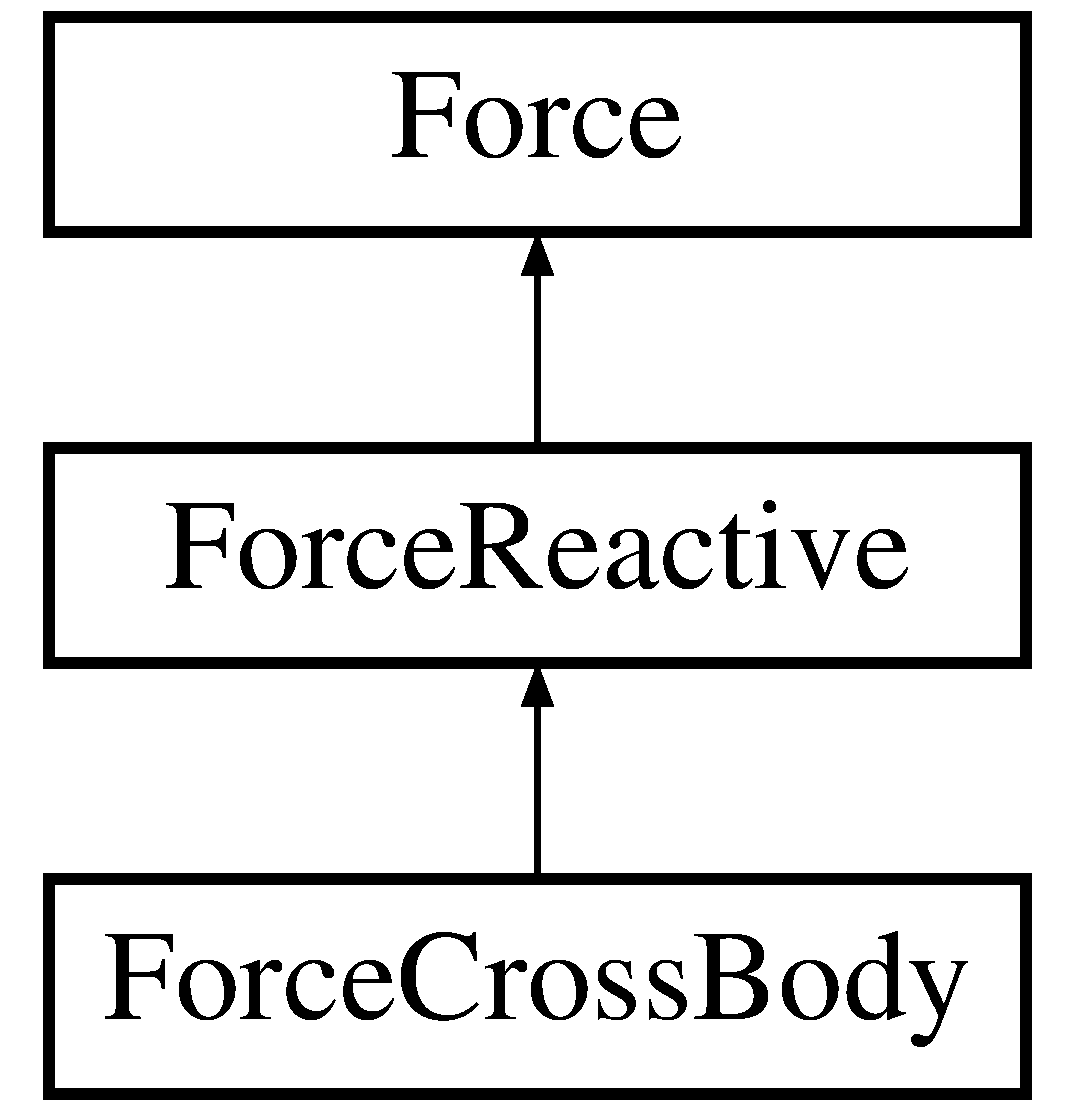
\includegraphics[height=3.000000cm]{class_force_cross_body}
\end{center}
\end{figure}
\subsection*{Public Member Functions}
\begin{DoxyCompactItemize}
\item 
\hyperlink{class_force_cross_body_a722c4ffad05245be224190bde22c6607}{Force\-Cross\-Body} ()
\item 
\hyperlink{class_force_cross_body_aaac5e33c56dcd4aee27f1e5ce1a0afa5}{$\sim$\-Force\-Cross\-Body} ()
\item 
void \hyperlink{class_force_cross_body_ab6bb83f04e9eec3b537b2570d712b3f8}{test\-Print} ()
\end{DoxyCompactItemize}
\subsection*{Additional Inherited Members}


\subsection{Detailed Description}
This class holds data for a cross body force. 

\subsection{Constructor \& Destructor Documentation}
\hypertarget{class_force_cross_body_a722c4ffad05245be224190bde22c6607}{\index{Force\-Cross\-Body@{Force\-Cross\-Body}!Force\-Cross\-Body@{Force\-Cross\-Body}}
\index{Force\-Cross\-Body@{Force\-Cross\-Body}!ForceCrossBody@{Force\-Cross\-Body}}
\subsubsection[{Force\-Cross\-Body}]{\setlength{\rightskip}{0pt plus 5cm}Force\-Cross\-Body\-::\-Force\-Cross\-Body (
\begin{DoxyParamCaption}
{}
\end{DoxyParamCaption}
)}}\label{class_force_cross_body_a722c4ffad05245be224190bde22c6607}
This default constructor creates a \hyperlink{class_body}{Body} object. \hypertarget{class_force_cross_body_aaac5e33c56dcd4aee27f1e5ce1a0afa5}{\index{Force\-Cross\-Body@{Force\-Cross\-Body}!$\sim$\-Force\-Cross\-Body@{$\sim$\-Force\-Cross\-Body}}
\index{$\sim$\-Force\-Cross\-Body@{$\sim$\-Force\-Cross\-Body}!ForceCrossBody@{Force\-Cross\-Body}}
\subsubsection[{$\sim$\-Force\-Cross\-Body}]{\setlength{\rightskip}{0pt plus 5cm}Force\-Cross\-Body\-::$\sim$\-Force\-Cross\-Body (
\begin{DoxyParamCaption}
{}
\end{DoxyParamCaption}
)}}\label{class_force_cross_body_aaac5e33c56dcd4aee27f1e5ce1a0afa5}
The default destructor, nothing happens here. 

\subsection{Member Function Documentation}
\hypertarget{class_force_cross_body_ab6bb83f04e9eec3b537b2570d712b3f8}{\index{Force\-Cross\-Body@{Force\-Cross\-Body}!test\-Print@{test\-Print}}
\index{test\-Print@{test\-Print}!ForceCrossBody@{Force\-Cross\-Body}}
\subsubsection[{test\-Print}]{\setlength{\rightskip}{0pt plus 5cm}void Force\-Cross\-Body\-::test\-Print (
\begin{DoxyParamCaption}
{}
\end{DoxyParamCaption}
)}}\label{class_force_cross_body_ab6bb83f04e9eec3b537b2570d712b3f8}
Test print to console the values of all data members. 

The documentation for this class was generated from the following files\-:\begin{DoxyCompactItemize}
\item 
Visual Studio 2010/\-Projects/o\-Freq Windows V\-S2010/o\-Freq/forcecrossbody.\-h\item 
Visual Studio 2010/\-Projects/o\-Freq Windows V\-S2010/o\-Freq/forcecrossbody.\-cpp\end{DoxyCompactItemize}

\hypertarget{class_force_reactive}{\section{Force\-Reactive Class Reference}
\label{class_force_reactive}\index{Force\-Reactive@{Force\-Reactive}}
}


{\ttfamily \#include $<$forcereactive.\-h$>$}

Inheritance diagram for Force\-Reactive\-:\begin{figure}[H]
\begin{center}
\leavevmode
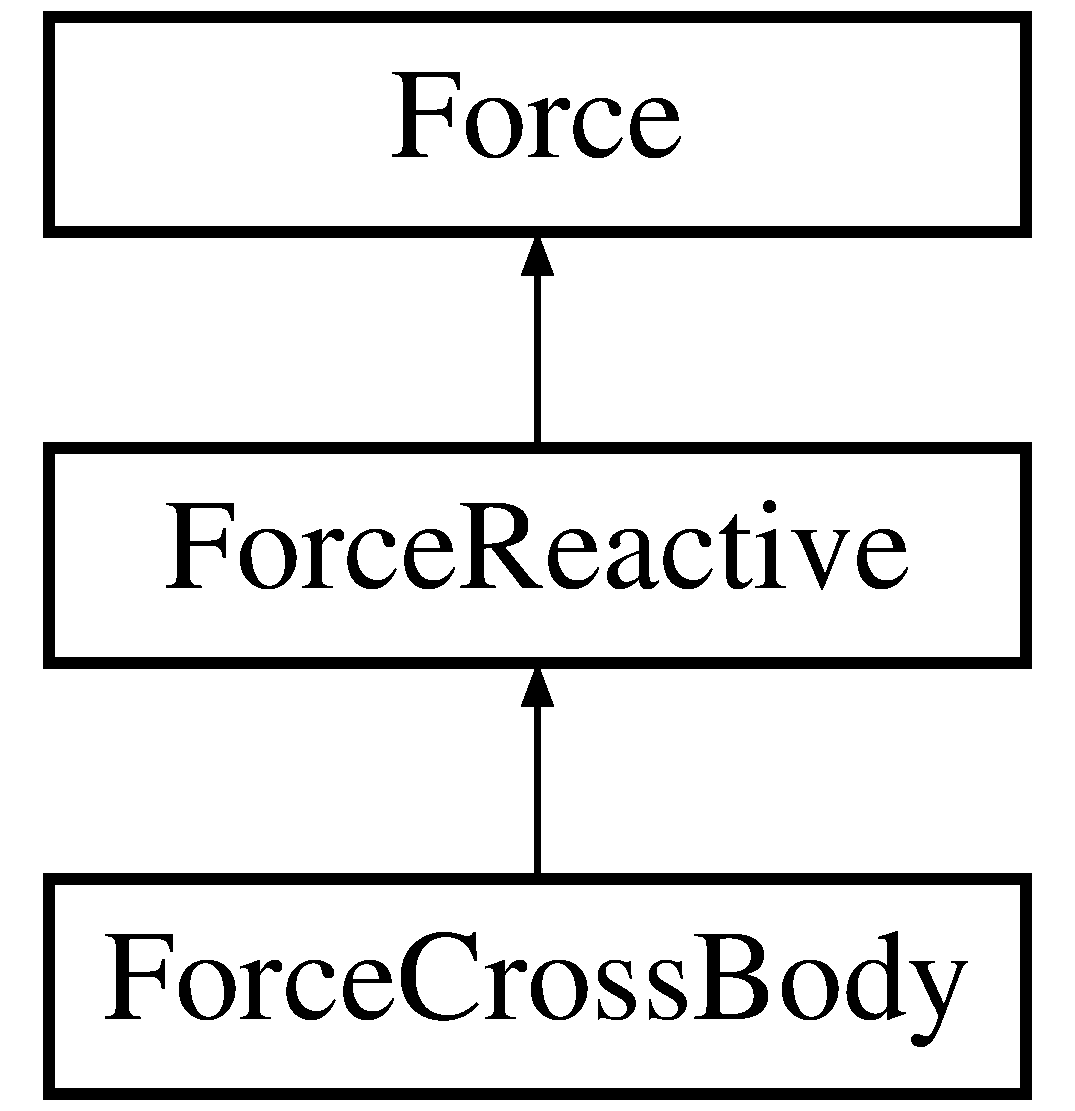
\includegraphics[height=3.000000cm]{class_force_reactive}
\end{center}
\end{figure}
\subsection*{Public Member Functions}
\begin{DoxyCompactItemize}
\item 
\hyperlink{class_force_reactive_a620cb084872d0d7e1c5d596fc05b00e5}{Force\-Reactive} ()
\item 
\hyperlink{class_force_reactive_abb3aceb796c02f9289b6b270a36d1a9d}{$\sim$\-Force\-Reactive} ()
\item 
void \hyperlink{class_force_reactive_adc057ed59345c6f7a8f522e80ab9be08}{test\-Print} ()
\item 
void \hyperlink{class_force_reactive_a2594a1dd03dd983e7eb4204148698c34}{set\-Coeff} (vector$<$ string $>$, bool)
\item 
void \hyperlink{class_force_reactive_a6f1969b59143d74dfd05006dcb18414d}{set\-Cur\-Derivative} (int)
\item 
void \hyperlink{class_force_reactive_a6e1a59348fb32dc15a6918bfc42a4cad}{set\-Cur\-Equation\-Num} (int)
\item 
vector$<$ \hyperlink{class_derivative}{Derivative} $>$ \hyperlink{class_force_reactive_aff4ed3ee3ba6ff0b013fb02183c01af8}{get\-Derivatives} ()
\end{DoxyCompactItemize}
\subsection*{Protected Attributes}
\begin{DoxyCompactItemize}
\item 
\hyperlink{class_derivative}{Derivative} \hyperlink{class_force_reactive_ad0da544a781cfac29d317e8c59e9f3f0}{derivative} \mbox{[}M\-A\-X\-\_\-\-O\-R\-D\-E\-R\-\_\-\-D\-E\-R\-I\-V\-A\-T\-I\-V\-E\mbox{]}
\item 
int \hyperlink{class_force_reactive_a6c4302050614499c9ffeda4ad21928ec}{current\-Derivative}
\item 
int \hyperlink{class_force_reactive_a9aa1f30d63006bc56be33830da1d8331}{current\-Equation}
\end{DoxyCompactItemize}


\subsection{Detailed Description}
This class holds all of the data for a reactive force. 

\subsection{Constructor \& Destructor Documentation}
\hypertarget{class_force_reactive_a620cb084872d0d7e1c5d596fc05b00e5}{\index{Force\-Reactive@{Force\-Reactive}!Force\-Reactive@{Force\-Reactive}}
\index{Force\-Reactive@{Force\-Reactive}!ForceReactive@{Force\-Reactive}}
\subsubsection[{Force\-Reactive}]{\setlength{\rightskip}{0pt plus 5cm}Force\-Reactive\-::\-Force\-Reactive (
\begin{DoxyParamCaption}
{}
\end{DoxyParamCaption}
)}}\label{class_force_reactive_a620cb084872d0d7e1c5d596fc05b00e5}
This default constructor. \hypertarget{class_force_reactive_abb3aceb796c02f9289b6b270a36d1a9d}{\index{Force\-Reactive@{Force\-Reactive}!$\sim$\-Force\-Reactive@{$\sim$\-Force\-Reactive}}
\index{$\sim$\-Force\-Reactive@{$\sim$\-Force\-Reactive}!ForceReactive@{Force\-Reactive}}
\subsubsection[{$\sim$\-Force\-Reactive}]{\setlength{\rightskip}{0pt plus 5cm}Force\-Reactive\-::$\sim$\-Force\-Reactive (
\begin{DoxyParamCaption}
{}
\end{DoxyParamCaption}
)}}\label{class_force_reactive_abb3aceb796c02f9289b6b270a36d1a9d}
The default destructor, nothing happens here. 

\subsection{Member Function Documentation}
\hypertarget{class_force_reactive_aff4ed3ee3ba6ff0b013fb02183c01af8}{\index{Force\-Reactive@{Force\-Reactive}!get\-Derivatives@{get\-Derivatives}}
\index{get\-Derivatives@{get\-Derivatives}!ForceReactive@{Force\-Reactive}}
\subsubsection[{get\-Derivatives}]{\setlength{\rightskip}{0pt plus 5cm}vector$<$ {\bf Derivative} $>$ Force\-Reactive\-::get\-Derivatives (
\begin{DoxyParamCaption}
{}
\end{DoxyParamCaption}
)}}\label{class_force_reactive_aff4ed3ee3ba6ff0b013fb02183c01af8}
Retrieve the order derivative \begin{DoxyReturn}{Returns}
The order derivative of this object. 
\end{DoxyReturn}
\hypertarget{class_force_reactive_a2594a1dd03dd983e7eb4204148698c34}{\index{Force\-Reactive@{Force\-Reactive}!set\-Coeff@{set\-Coeff}}
\index{set\-Coeff@{set\-Coeff}!ForceReactive@{Force\-Reactive}}
\subsubsection[{set\-Coeff}]{\setlength{\rightskip}{0pt plus 5cm}void Force\-Reactive\-::set\-Coeff (
\begin{DoxyParamCaption}
\item[{vector$<$ string $>$}]{new\-List, }
\item[{bool}]{is\-Direct\-List}
\end{DoxyParamCaption}
)}}\label{class_force_reactive_a2594a1dd03dd983e7eb4204148698c34}
Sets the list of coeffcients. 
\begin{DoxyParams}{Parameters}
{\em new\-List} & The list of coefficients. \\
\hline
{\em is\-Direct\-List} & Specifies whether the list is direct or sequential. \\
\hline
\end{DoxyParams}
\hypertarget{class_force_reactive_a6f1969b59143d74dfd05006dcb18414d}{\index{Force\-Reactive@{Force\-Reactive}!set\-Cur\-Derivative@{set\-Cur\-Derivative}}
\index{set\-Cur\-Derivative@{set\-Cur\-Derivative}!ForceReactive@{Force\-Reactive}}
\subsubsection[{set\-Cur\-Derivative}]{\setlength{\rightskip}{0pt plus 5cm}void Force\-Reactive\-::set\-Cur\-Derivative (
\begin{DoxyParamCaption}
\item[{int}]{new\-Order}
\end{DoxyParamCaption}
)}}\label{class_force_reactive_a6f1969b59143d74dfd05006dcb18414d}
Sets the current derivative. 
\begin{DoxyParams}{Parameters}
{\em neworder} & The order of derivative. \\
\hline
\end{DoxyParams}
\hypertarget{class_force_reactive_a6e1a59348fb32dc15a6918bfc42a4cad}{\index{Force\-Reactive@{Force\-Reactive}!set\-Cur\-Equation\-Num@{set\-Cur\-Equation\-Num}}
\index{set\-Cur\-Equation\-Num@{set\-Cur\-Equation\-Num}!ForceReactive@{Force\-Reactive}}
\subsubsection[{set\-Cur\-Equation\-Num}]{\setlength{\rightskip}{0pt plus 5cm}void Force\-Reactive\-::set\-Cur\-Equation\-Num (
\begin{DoxyParamCaption}
\item[{int}]{new\-Equation\-Num}
\end{DoxyParamCaption}
)}}\label{class_force_reactive_a6e1a59348fb32dc15a6918bfc42a4cad}
Sets the current number of the equation. 
\begin{DoxyParams}{Parameters}
{\em new\-Equation\-Num} & The number of the equation. \\
\hline
\end{DoxyParams}
\hypertarget{class_force_reactive_adc057ed59345c6f7a8f522e80ab9be08}{\index{Force\-Reactive@{Force\-Reactive}!test\-Print@{test\-Print}}
\index{test\-Print@{test\-Print}!ForceReactive@{Force\-Reactive}}
\subsubsection[{test\-Print}]{\setlength{\rightskip}{0pt plus 5cm}void Force\-Reactive\-::test\-Print (
\begin{DoxyParamCaption}
{}
\end{DoxyParamCaption}
)}}\label{class_force_reactive_adc057ed59345c6f7a8f522e80ab9be08}
Test print to console the values of all data members. 

\subsection{Member Data Documentation}
\hypertarget{class_force_reactive_a6c4302050614499c9ffeda4ad21928ec}{\index{Force\-Reactive@{Force\-Reactive}!current\-Derivative@{current\-Derivative}}
\index{current\-Derivative@{current\-Derivative}!ForceReactive@{Force\-Reactive}}
\subsubsection[{current\-Derivative}]{\setlength{\rightskip}{0pt plus 5cm}int Force\-Reactive\-::current\-Derivative\hspace{0.3cm}{\ttfamily [protected]}}}\label{class_force_reactive_a6c4302050614499c9ffeda4ad21928ec}
The current order derivative. \hypertarget{class_force_reactive_a9aa1f30d63006bc56be33830da1d8331}{\index{Force\-Reactive@{Force\-Reactive}!current\-Equation@{current\-Equation}}
\index{current\-Equation@{current\-Equation}!ForceReactive@{Force\-Reactive}}
\subsubsection[{current\-Equation}]{\setlength{\rightskip}{0pt plus 5cm}int Force\-Reactive\-::current\-Equation\hspace{0.3cm}{\ttfamily [protected]}}}\label{class_force_reactive_a9aa1f30d63006bc56be33830da1d8331}
This current equation number. \hypertarget{class_force_reactive_ad0da544a781cfac29d317e8c59e9f3f0}{\index{Force\-Reactive@{Force\-Reactive}!derivative@{derivative}}
\index{derivative@{derivative}!ForceReactive@{Force\-Reactive}}
\subsubsection[{derivative}]{\setlength{\rightskip}{0pt plus 5cm}{\bf Derivative} Force\-Reactive\-::derivative\mbox{[}M\-A\-X\-\_\-\-O\-R\-D\-E\-R\-\_\-\-D\-E\-R\-I\-V\-A\-T\-I\-V\-E\mbox{]}\hspace{0.3cm}{\ttfamily [protected]}}}\label{class_force_reactive_ad0da544a781cfac29d317e8c59e9f3f0}
This list of derivatives. 

The documentation for this class was generated from the following files\-:\begin{DoxyCompactItemize}
\item 
Visual Studio 2010/\-Projects/o\-Freq Windows V\-S2010/o\-Freq/forcereactive.\-h\item 
Visual Studio 2010/\-Projects/o\-Freq Windows V\-S2010/o\-Freq/forcereactive.\-cpp\end{DoxyCompactItemize}

\hypertarget{class_forces_input}{\section{Forces\-Input Class Reference}
\label{class_forces_input}\index{Forces\-Input@{Forces\-Input}}
}


{\ttfamily \#include $<$forcesinput.\-h$>$}

Inheritance diagram for Forces\-Input\-:\begin{figure}[H]
\begin{center}
\leavevmode
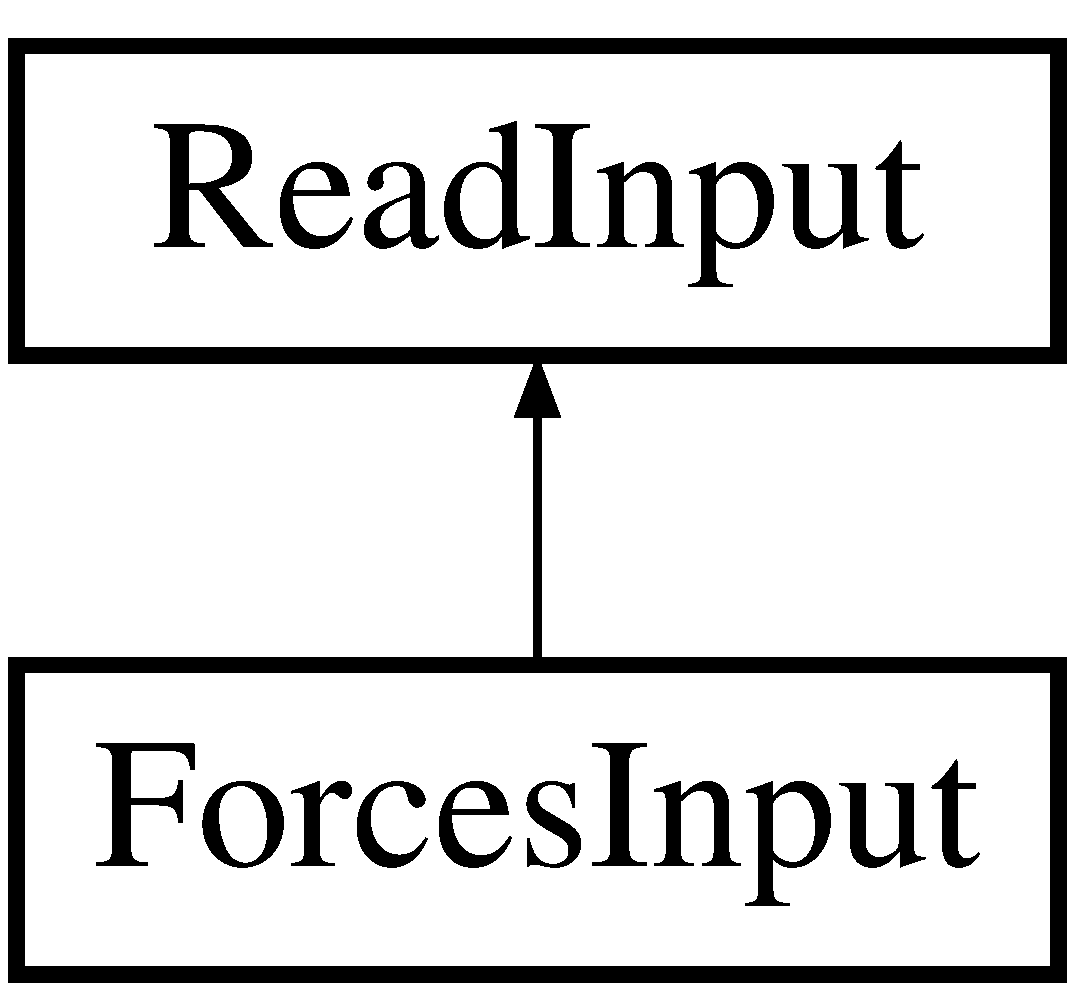
\includegraphics[height=2.000000cm]{class_forces_input}
\end{center}
\end{figure}
\subsection*{Public Member Functions}
\begin{DoxyCompactItemize}
\item 
\hyperlink{class_forces_input_ad3da9dd7decddd74ba054f3e58a848fe}{Forces\-Input} ()
\item 
\hyperlink{class_forces_input_a5891d1dd81b2e4202fe023985aa0ff1b}{$\sim$\-Forces\-Input} ()
\item 
void \hyperlink{class_forces_input_af9ca173b1f53914ba8f118ae2cc211a3}{test\-Print} ()
\item 
\hyperlink{class_user_forces}{User\-Forces} \hyperlink{class_forces_input_ab5262ae1b53c658dbaab66d338e465e2}{get\-User\-Forces} ()
\end{DoxyCompactItemize}
\subsection*{Protected Member Functions}
\begin{DoxyCompactItemize}
\item 
void \hyperlink{class_forces_input_a8bcfe50a80d1c2fe11a742081a5e7343}{initialize\-Defaults} ()
\item 
int \hyperlink{class_forces_input_a5f4086acc636b54b64bcd611bdff1aa4}{legal\-Keyword} (string)
\item 
bool \hyperlink{class_forces_input_a3e82ee7aa3c5bd35a6bb1b06fcafafa9}{keyword\-Handler} (int, string, string)
\item 
bool \hyperlink{class_forces_input_a52965f2bfde734252e7f4f65bf0fde25}{keyword\-Handler} (int, vector$<$ string $>$, bool)
\end{DoxyCompactItemize}


\subsection{Detailed Description}
This class parses input from file and stores the data appropriately in the \hyperlink{class_user_forces}{User\-Forces} object. 

\subsection{Constructor \& Destructor Documentation}
\hypertarget{class_forces_input_ad3da9dd7decddd74ba054f3e58a848fe}{\index{Forces\-Input@{Forces\-Input}!Forces\-Input@{Forces\-Input}}
\index{Forces\-Input@{Forces\-Input}!ForcesInput@{Forces\-Input}}
\subsubsection[{Forces\-Input}]{\setlength{\rightskip}{0pt plus 5cm}Forces\-Input\-::\-Forces\-Input (
\begin{DoxyParamCaption}
{}
\end{DoxyParamCaption}
)}}\label{class_forces_input_ad3da9dd7decddd74ba054f3e58a848fe}
The default constructor. \hypertarget{class_forces_input_a5891d1dd81b2e4202fe023985aa0ff1b}{\index{Forces\-Input@{Forces\-Input}!$\sim$\-Forces\-Input@{$\sim$\-Forces\-Input}}
\index{$\sim$\-Forces\-Input@{$\sim$\-Forces\-Input}!ForcesInput@{Forces\-Input}}
\subsubsection[{$\sim$\-Forces\-Input}]{\setlength{\rightskip}{0pt plus 5cm}Forces\-Input\-::$\sim$\-Forces\-Input (
\begin{DoxyParamCaption}
{}
\end{DoxyParamCaption}
)}}\label{class_forces_input_a5891d1dd81b2e4202fe023985aa0ff1b}
The default destructor, nothing happens here. 

\subsection{Member Function Documentation}
\hypertarget{class_forces_input_ab5262ae1b53c658dbaab66d338e465e2}{\index{Forces\-Input@{Forces\-Input}!get\-User\-Forces@{get\-User\-Forces}}
\index{get\-User\-Forces@{get\-User\-Forces}!ForcesInput@{Forces\-Input}}
\subsubsection[{get\-User\-Forces}]{\setlength{\rightskip}{0pt plus 5cm}{\bf User\-Forces} Forces\-Input\-::get\-User\-Forces (
\begin{DoxyParamCaption}
{}
\end{DoxyParamCaption}
)}}\label{class_forces_input_ab5262ae1b53c658dbaab66d338e465e2}
Returns user forces. \hypertarget{class_forces_input_a8bcfe50a80d1c2fe11a742081a5e7343}{\index{Forces\-Input@{Forces\-Input}!initialize\-Defaults@{initialize\-Defaults}}
\index{initialize\-Defaults@{initialize\-Defaults}!ForcesInput@{Forces\-Input}}
\subsubsection[{initialize\-Defaults}]{\setlength{\rightskip}{0pt plus 5cm}void Forces\-Input\-::initialize\-Defaults (
\begin{DoxyParamCaption}
{}
\end{DoxyParamCaption}
)\hspace{0.3cm}{\ttfamily [protected]}, {\ttfamily [virtual]}}}\label{class_forces_input_a8bcfe50a80d1c2fe11a742081a5e7343}
For future use, does nothing as of now. 

Implements \hyperlink{class_read_input_a4ff2727b876cfd7c01299b08bdd65646}{Read\-Input}.

\hypertarget{class_forces_input_a3e82ee7aa3c5bd35a6bb1b06fcafafa9}{\index{Forces\-Input@{Forces\-Input}!keyword\-Handler@{keyword\-Handler}}
\index{keyword\-Handler@{keyword\-Handler}!ForcesInput@{Forces\-Input}}
\subsubsection[{keyword\-Handler}]{\setlength{\rightskip}{0pt plus 5cm}bool Forces\-Input\-::keyword\-Handler (
\begin{DoxyParamCaption}
\item[{int}]{key\-Control, }
\item[{string}]{identifier, }
\item[{string}]{val}
\end{DoxyParamCaption}
)\hspace{0.3cm}{\ttfamily [protected]}, {\ttfamily [virtual]}}}\label{class_forces_input_a3e82ee7aa3c5bd35a6bb1b06fcafafa9}
Stores the data if valid keyword according to the legeal\-Keyword function. 
\begin{DoxyParams}{Parameters}
{\em key\-Control} & Indicated which case in switch function to use. \\
\hline
{\em identifier} & The keyword. \\
\hline
{\em val} & The value associated with the keyword. \\
\hline
\end{DoxyParams}
\begin{DoxyReturn}{Returns}
false if not done reading data, true to move onto next keyword in parser. 
\end{DoxyReturn}


Implements \hyperlink{class_read_input_a1d8cb0ef59f265300b682de97513f48d}{Read\-Input}.

\hypertarget{class_forces_input_a52965f2bfde734252e7f4f65bf0fde25}{\index{Forces\-Input@{Forces\-Input}!keyword\-Handler@{keyword\-Handler}}
\index{keyword\-Handler@{keyword\-Handler}!ForcesInput@{Forces\-Input}}
\subsubsection[{keyword\-Handler}]{\setlength{\rightskip}{0pt plus 5cm}bool Forces\-Input\-::keyword\-Handler (
\begin{DoxyParamCaption}
\item[{int}]{key\-Control, }
\item[{vector$<$ string $>$}]{the\-List\-In, }
\item[{bool}]{is\-Direct}
\end{DoxyParamCaption}
)\hspace{0.3cm}{\ttfamily [protected]}, {\ttfamily [virtual]}}}\label{class_forces_input_a52965f2bfde734252e7f4f65bf0fde25}
Stores the list data if valid keyword according to the legeal\-Keyword function. 
\begin{DoxyParams}{Parameters}
{\em key\-Control} & Indicated which case in switch function to use. \\
\hline
{\em the\-List\-In} & List of Values. \\
\hline
{\em is\-Direct} & True if Direct Access List, False if Sequenctial List. \\
\hline
\end{DoxyParams}
\begin{DoxyReturn}{Returns}
false if not done reading data, true to move onto next keyword in parser. 
\end{DoxyReturn}


Implements \hyperlink{class_read_input_afb66a7ff67d0aeb10a3cfa5a4fbc31f8}{Read\-Input}.

\hypertarget{class_forces_input_a5f4086acc636b54b64bcd611bdff1aa4}{\index{Forces\-Input@{Forces\-Input}!legal\-Keyword@{legal\-Keyword}}
\index{legal\-Keyword@{legal\-Keyword}!ForcesInput@{Forces\-Input}}
\subsubsection[{legal\-Keyword}]{\setlength{\rightskip}{0pt plus 5cm}int Forces\-Input\-::legal\-Keyword (
\begin{DoxyParamCaption}
\item[{string}]{string\-In}
\end{DoxyParamCaption}
)\hspace{0.3cm}{\ttfamily [protected]}, {\ttfamily [virtual]}}}\label{class_forces_input_a5f4086acc636b54b64bcd611bdff1aa4}
Returns int greater than 0 if the keyword is legal, the int returned specifies how to handle data in keyword\-Handler. 
\begin{DoxyParams}{Parameters}
{\em string\-In} & Check if a valid keyword. \\
\hline
\end{DoxyParams}
\begin{DoxyReturn}{Returns}
int value which tells keyword\-Handler how to handle the data. 
\end{DoxyReturn}


Implements \hyperlink{class_read_input_a4c67f10e813686bf635dd4c6bb2c61bc}{Read\-Input}.

\hypertarget{class_forces_input_af9ca173b1f53914ba8f118ae2cc211a3}{\index{Forces\-Input@{Forces\-Input}!test\-Print@{test\-Print}}
\index{test\-Print@{test\-Print}!ForcesInput@{Forces\-Input}}
\subsubsection[{test\-Print}]{\setlength{\rightskip}{0pt plus 5cm}void Forces\-Input\-::test\-Print (
\begin{DoxyParamCaption}
{}
\end{DoxyParamCaption}
)}}\label{class_forces_input_af9ca173b1f53914ba8f118ae2cc211a3}
Print to console all data members. 

The documentation for this class was generated from the following files\-:\begin{DoxyCompactItemize}
\item 
Visual Studio 2010/\-Projects/o\-Freq Windows V\-S2010/o\-Freq/forcesinput.\-h\item 
Visual Studio 2010/\-Projects/o\-Freq Windows V\-S2010/o\-Freq/forcesinput.\-cpp\end{DoxyCompactItemize}

\hypertarget{class_global_acceleration}{\section{Global\-Acceleration Class Reference}
\label{class_global_acceleration}\index{Global\-Acceleration@{Global\-Acceleration}}
}


{\ttfamily \#include $<$globalacceleration.\-h$>$}

Inheritance diagram for Global\-Acceleration\-:\begin{figure}[H]
\begin{center}
\leavevmode
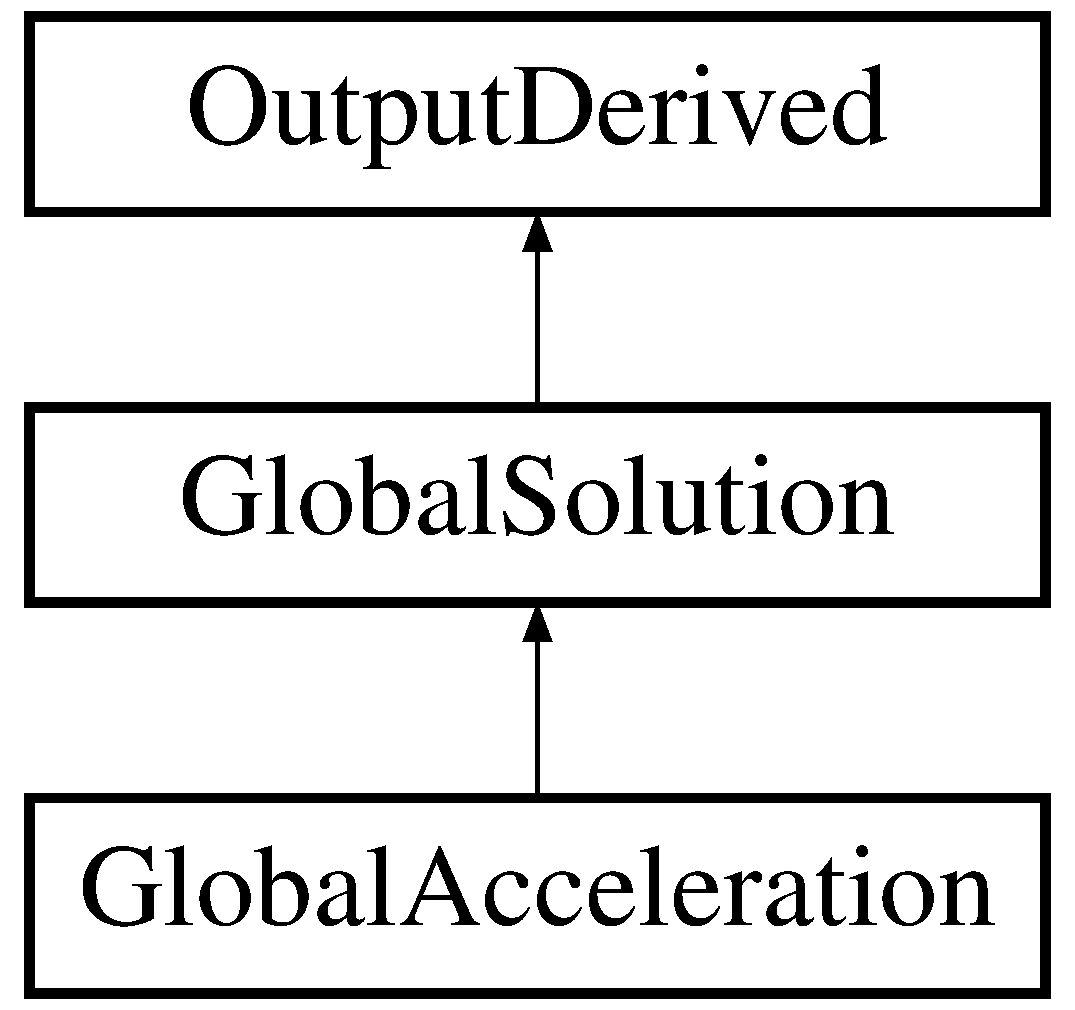
\includegraphics[height=3.000000cm]{class_global_acceleration}
\end{center}
\end{figure}
\subsection*{Public Member Functions}
\begin{DoxyCompactItemize}
\item 
\hyperlink{class_global_acceleration_a37a05fcecd06641847388428a3f43fb8}{Global\-Acceleration} ()
\item 
\hyperlink{class_global_acceleration_aafb7853a1923f0e06b96f2ef4eca03d3}{$\sim$\-Global\-Acceleration} ()
\end{DoxyCompactItemize}
\subsection*{Additional Inherited Members}


\subsection{Detailed Description}
This class represents the Global Acceleraion Solution. 

\subsection{Constructor \& Destructor Documentation}
\hypertarget{class_global_acceleration_a37a05fcecd06641847388428a3f43fb8}{\index{Global\-Acceleration@{Global\-Acceleration}!Global\-Acceleration@{Global\-Acceleration}}
\index{Global\-Acceleration@{Global\-Acceleration}!GlobalAcceleration@{Global\-Acceleration}}
\subsubsection[{Global\-Acceleration}]{\setlength{\rightskip}{0pt plus 5cm}Global\-Acceleration\-::\-Global\-Acceleration (
\begin{DoxyParamCaption}
{}
\end{DoxyParamCaption}
)}}\label{class_global_acceleration_a37a05fcecd06641847388428a3f43fb8}
This default constructor creates a Global Acceleration object. \hypertarget{class_global_acceleration_aafb7853a1923f0e06b96f2ef4eca03d3}{\index{Global\-Acceleration@{Global\-Acceleration}!$\sim$\-Global\-Acceleration@{$\sim$\-Global\-Acceleration}}
\index{$\sim$\-Global\-Acceleration@{$\sim$\-Global\-Acceleration}!GlobalAcceleration@{Global\-Acceleration}}
\subsubsection[{$\sim$\-Global\-Acceleration}]{\setlength{\rightskip}{0pt plus 5cm}Global\-Acceleration\-::$\sim$\-Global\-Acceleration (
\begin{DoxyParamCaption}
{}
\end{DoxyParamCaption}
)}}\label{class_global_acceleration_aafb7853a1923f0e06b96f2ef4eca03d3}
The default destructor, nothing happens here. 

The documentation for this class was generated from the following files\-:\begin{DoxyCompactItemize}
\item 
Visual Studio 2010/\-Projects/o\-Freq Windows V\-S2010/o\-Freq/globalacceleration.\-h\item 
Visual Studio 2010/\-Projects/o\-Freq Windows V\-S2010/o\-Freq/globalacceleration.\-cpp\end{DoxyCompactItemize}

\hypertarget{class_global_motion}{\section{Global\-Motion Class Reference}
\label{class_global_motion}\index{Global\-Motion@{Global\-Motion}}
}


{\ttfamily \#include $<$globalmotion.\-h$>$}

Inheritance diagram for Global\-Motion\-:\begin{figure}[H]
\begin{center}
\leavevmode
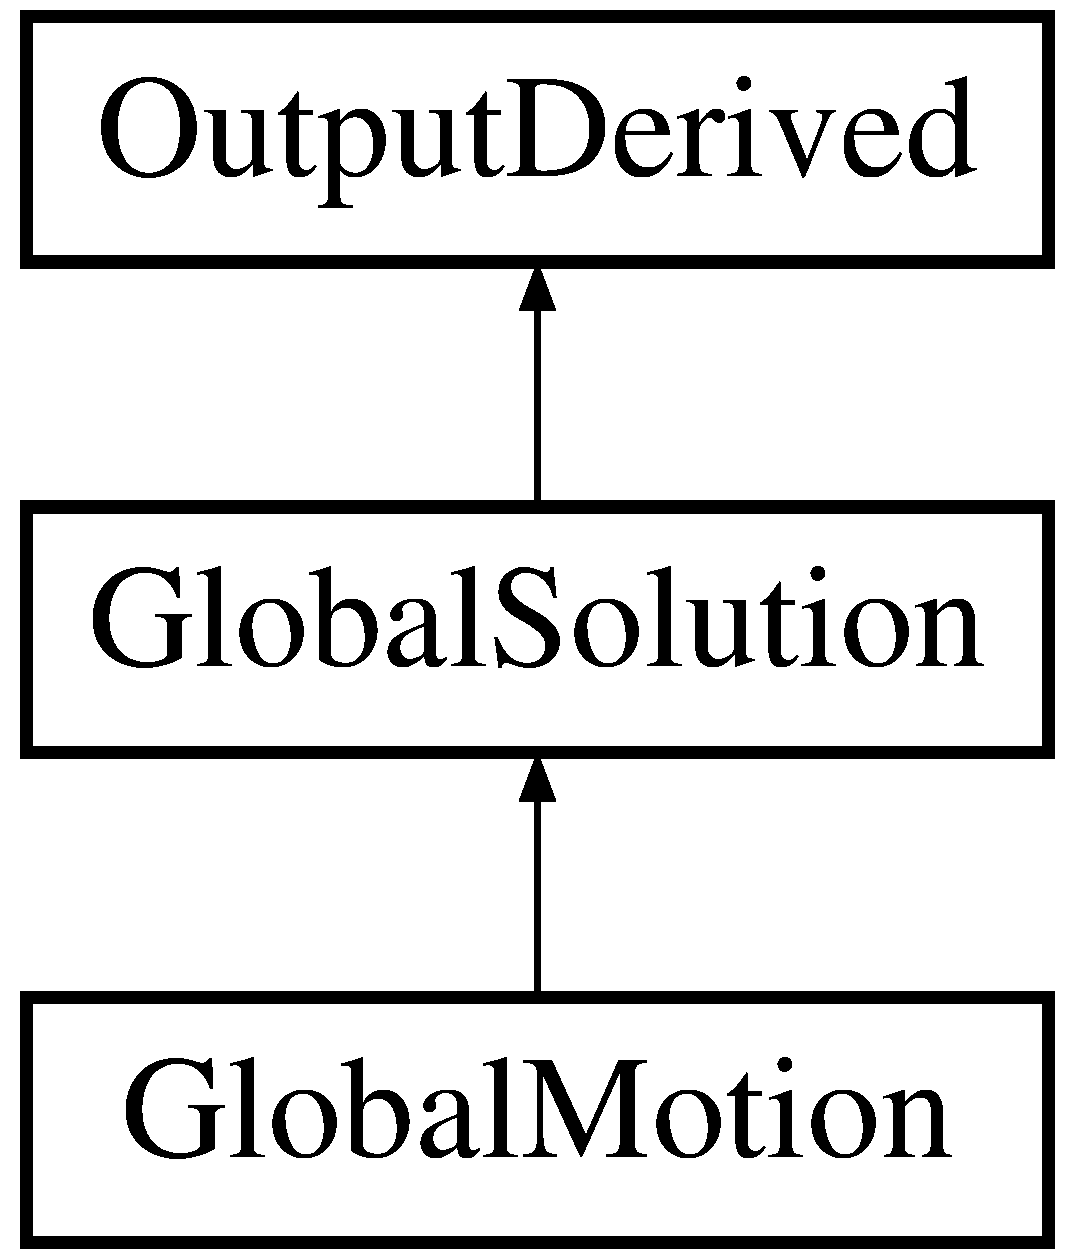
\includegraphics[height=3.000000cm]{class_global_motion}
\end{center}
\end{figure}
\subsection*{Public Member Functions}
\begin{DoxyCompactItemize}
\item 
\hyperlink{class_global_motion_afe0b801895608782addf27d231bce572}{Global\-Motion} ()
\item 
\hyperlink{class_global_motion_aee21eade3de9cb666a6b8fa42cf1e9e1}{$\sim$\-Global\-Motion} ()
\end{DoxyCompactItemize}
\subsection*{Additional Inherited Members}


\subsection{Detailed Description}
This class represents the Global Motion Solution. 

\subsection{Constructor \& Destructor Documentation}
\hypertarget{class_global_motion_afe0b801895608782addf27d231bce572}{\index{Global\-Motion@{Global\-Motion}!Global\-Motion@{Global\-Motion}}
\index{Global\-Motion@{Global\-Motion}!GlobalMotion@{Global\-Motion}}
\subsubsection[{Global\-Motion}]{\setlength{\rightskip}{0pt plus 5cm}Global\-Motion\-::\-Global\-Motion (
\begin{DoxyParamCaption}
{}
\end{DoxyParamCaption}
)}}\label{class_global_motion_afe0b801895608782addf27d231bce572}
This default constructor creates a Global Motion object. \hypertarget{class_global_motion_aee21eade3de9cb666a6b8fa42cf1e9e1}{\index{Global\-Motion@{Global\-Motion}!$\sim$\-Global\-Motion@{$\sim$\-Global\-Motion}}
\index{$\sim$\-Global\-Motion@{$\sim$\-Global\-Motion}!GlobalMotion@{Global\-Motion}}
\subsubsection[{$\sim$\-Global\-Motion}]{\setlength{\rightskip}{0pt plus 5cm}Global\-Motion\-::$\sim$\-Global\-Motion (
\begin{DoxyParamCaption}
{}
\end{DoxyParamCaption}
)}}\label{class_global_motion_aee21eade3de9cb666a6b8fa42cf1e9e1}
The default destructor, nothing happens here. 

The documentation for this class was generated from the following files\-:\begin{DoxyCompactItemize}
\item 
Visual Studio 2010/\-Projects/o\-Freq Windows V\-S2010/o\-Freq/globalmotion.\-h\item 
Visual Studio 2010/\-Projects/o\-Freq Windows V\-S2010/o\-Freq/globalmotion.\-cpp\end{DoxyCompactItemize}

\hypertarget{class_global_solution}{\section{Global\-Solution Class Reference}
\label{class_global_solution}\index{Global\-Solution@{Global\-Solution}}
}


{\ttfamily \#include $<$globalsolution.\-h$>$}

Inheritance diagram for Global\-Solution\-:\begin{figure}[H]
\begin{center}
\leavevmode
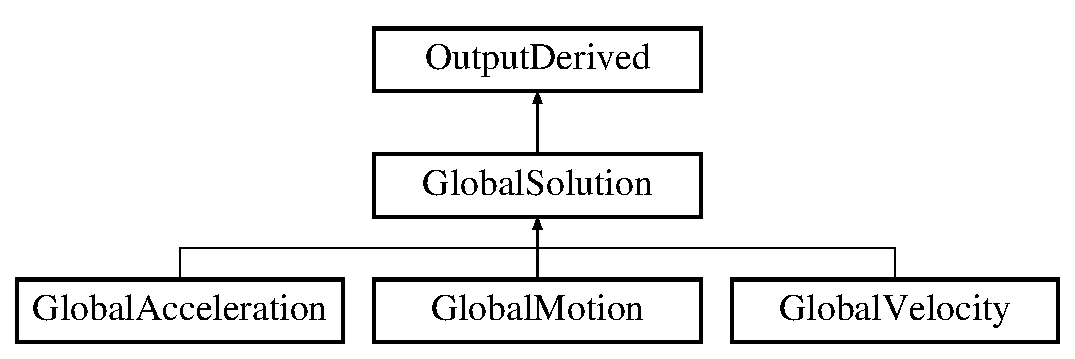
\includegraphics[height=3.000000cm]{class_global_solution}
\end{center}
\end{figure}
\subsection*{Public Member Functions}
\begin{DoxyCompactItemize}
\item 
\hyperlink{class_global_solution_a27fcfb056c30fc07f8937bc71ec677e6}{Global\-Solution} ()
\item 
\hyperlink{class_global_solution_aea630b237ced06e04c5ea00bf1bb9398}{$\sim$\-Global\-Solution} ()
\item 
virtual cx\-\_\-mat \hyperlink{class_global_solution_a15634073f63559cbfd65b32b79cd7fbd}{calculate\-Output} (cx\-\_\-mat, double)
\end{DoxyCompactItemize}
\subsection*{Public Attributes}
\begin{DoxyCompactItemize}
\item 
int \hyperlink{class_global_solution_a026746ffb8e416eb4142a058b108148c}{order\-Derivative}
\end{DoxyCompactItemize}


\subsection{Detailed Description}
This class represents the Global Solution. 

\subsection{Constructor \& Destructor Documentation}
\hypertarget{class_global_solution_a27fcfb056c30fc07f8937bc71ec677e6}{\index{Global\-Solution@{Global\-Solution}!Global\-Solution@{Global\-Solution}}
\index{Global\-Solution@{Global\-Solution}!GlobalSolution@{Global\-Solution}}
\subsubsection[{Global\-Solution}]{\setlength{\rightskip}{0pt plus 5cm}Global\-Solution\-::\-Global\-Solution (
\begin{DoxyParamCaption}
{}
\end{DoxyParamCaption}
)}}\label{class_global_solution_a27fcfb056c30fc07f8937bc71ec677e6}
This default constructor creates a Global Solution object. \hypertarget{class_global_solution_aea630b237ced06e04c5ea00bf1bb9398}{\index{Global\-Solution@{Global\-Solution}!$\sim$\-Global\-Solution@{$\sim$\-Global\-Solution}}
\index{$\sim$\-Global\-Solution@{$\sim$\-Global\-Solution}!GlobalSolution@{Global\-Solution}}
\subsubsection[{$\sim$\-Global\-Solution}]{\setlength{\rightskip}{0pt plus 5cm}Global\-Solution\-::$\sim$\-Global\-Solution (
\begin{DoxyParamCaption}
{}
\end{DoxyParamCaption}
)}}\label{class_global_solution_aea630b237ced06e04c5ea00bf1bb9398}
The default destructor, nothing happens here. 

\subsection{Member Function Documentation}
\hypertarget{class_global_solution_a15634073f63559cbfd65b32b79cd7fbd}{\index{Global\-Solution@{Global\-Solution}!calculate\-Output@{calculate\-Output}}
\index{calculate\-Output@{calculate\-Output}!GlobalSolution@{Global\-Solution}}
\subsubsection[{calculate\-Output}]{\setlength{\rightskip}{0pt plus 5cm}cx\-\_\-mat Global\-Solution\-::calculate\-Output (
\begin{DoxyParamCaption}
\item[{cx\-\_\-mat}]{matrix\-In, }
\item[{double}]{cur\-Wave\-Freq}
\end{DoxyParamCaption}
)\hspace{0.3cm}{\ttfamily [virtual]}}}\label{class_global_solution_a15634073f63559cbfd65b32b79cd7fbd}
Calculates the outputs for Global Solution children classes 
\begin{DoxyParams}{Parameters}
{\em matrix\-In} & The original Matrix that is used for calculations. \\
\hline
{\em cur\-Wave\-Freq} & The current wave frequency. \\
\hline
\end{DoxyParams}
\begin{DoxyReturn}{Returns}
The new matrix with calculations on each index. 
\end{DoxyReturn}


Implements \hyperlink{class_output_derived_a1e0052dd24822806481976e42a2f5f30}{Output\-Derived}.



\subsection{Member Data Documentation}
\hypertarget{class_global_solution_a026746ffb8e416eb4142a058b108148c}{\index{Global\-Solution@{Global\-Solution}!order\-Derivative@{order\-Derivative}}
\index{order\-Derivative@{order\-Derivative}!GlobalSolution@{Global\-Solution}}
\subsubsection[{order\-Derivative}]{\setlength{\rightskip}{0pt plus 5cm}int Global\-Solution\-::order\-Derivative}}\label{class_global_solution_a026746ffb8e416eb4142a058b108148c}
Set by child classes 

The documentation for this class was generated from the following files\-:\begin{DoxyCompactItemize}
\item 
Visual Studio 2010/\-Projects/o\-Freq Windows V\-S2010/o\-Freq/globalsolution.\-h\item 
Visual Studio 2010/\-Projects/o\-Freq Windows V\-S2010/o\-Freq/globalsolution.\-cpp\end{DoxyCompactItemize}

\hypertarget{class_global_velocity}{\section{Global\-Velocity Class Reference}
\label{class_global_velocity}\index{Global\-Velocity@{Global\-Velocity}}
}


{\ttfamily \#include $<$globalvelocity.\-h$>$}

Inheritance diagram for Global\-Velocity\-:\begin{figure}[H]
\begin{center}
\leavevmode
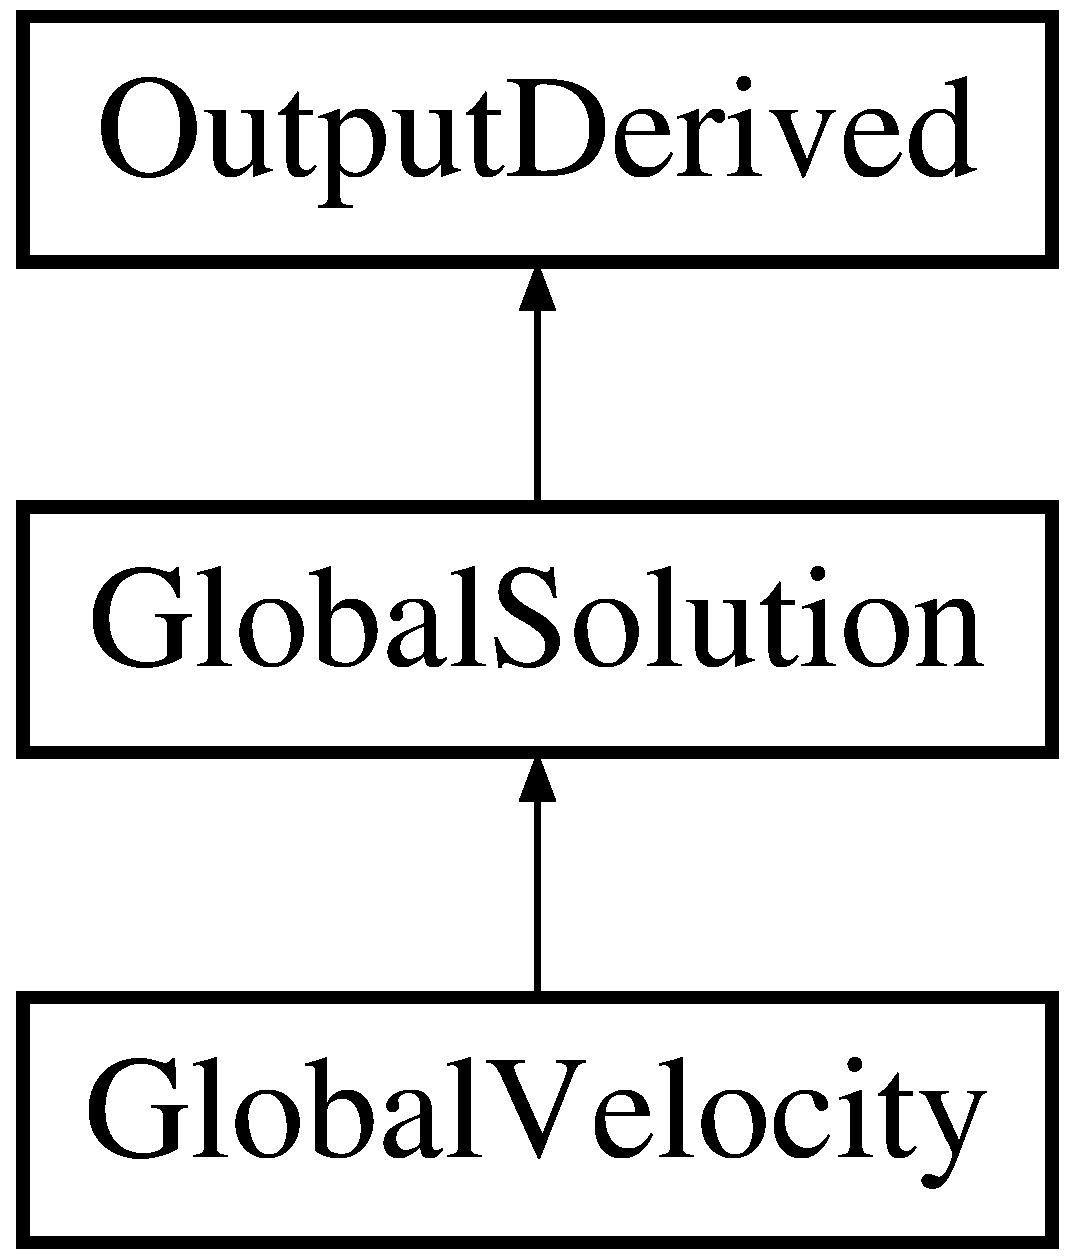
\includegraphics[height=3.000000cm]{class_global_velocity}
\end{center}
\end{figure}
\subsection*{Public Member Functions}
\begin{DoxyCompactItemize}
\item 
\hyperlink{class_global_velocity_a444ab39b351acd4e6ca7dc8088e2a9b8}{Global\-Velocity} ()
\item 
\hyperlink{class_global_velocity_a2b8f719180b1786a582d90603db8f2d8}{$\sim$\-Global\-Velocity} ()
\end{DoxyCompactItemize}
\subsection*{Additional Inherited Members}


\subsection{Detailed Description}
This class represents the Global Velocity Solution. 

\subsection{Constructor \& Destructor Documentation}
\hypertarget{class_global_velocity_a444ab39b351acd4e6ca7dc8088e2a9b8}{\index{Global\-Velocity@{Global\-Velocity}!Global\-Velocity@{Global\-Velocity}}
\index{Global\-Velocity@{Global\-Velocity}!GlobalVelocity@{Global\-Velocity}}
\subsubsection[{Global\-Velocity}]{\setlength{\rightskip}{0pt plus 5cm}Global\-Velocity\-::\-Global\-Velocity (
\begin{DoxyParamCaption}
{}
\end{DoxyParamCaption}
)}}\label{class_global_velocity_a444ab39b351acd4e6ca7dc8088e2a9b8}
This default constructor creates a Global Velocity object. \hypertarget{class_global_velocity_a2b8f719180b1786a582d90603db8f2d8}{\index{Global\-Velocity@{Global\-Velocity}!$\sim$\-Global\-Velocity@{$\sim$\-Global\-Velocity}}
\index{$\sim$\-Global\-Velocity@{$\sim$\-Global\-Velocity}!GlobalVelocity@{Global\-Velocity}}
\subsubsection[{$\sim$\-Global\-Velocity}]{\setlength{\rightskip}{0pt plus 5cm}Global\-Velocity\-::$\sim$\-Global\-Velocity (
\begin{DoxyParamCaption}
{}
\end{DoxyParamCaption}
)}}\label{class_global_velocity_a2b8f719180b1786a582d90603db8f2d8}
The default destructor, nothing happens here. 

The documentation for this class was generated from the following files\-:\begin{DoxyCompactItemize}
\item 
Visual Studio 2010/\-Projects/o\-Freq Windows V\-S2010/o\-Freq/globalvelocity.\-h\item 
Visual Studio 2010/\-Projects/o\-Freq Windows V\-S2010/o\-Freq/globalvelocity.\-cpp\end{DoxyCompactItemize}

\hypertarget{class_hydrodynamic_input}{\section{Hydrodynamic\-Input Class Reference}
\label{class_hydrodynamic_input}\index{Hydrodynamic\-Input@{Hydrodynamic\-Input}}
}
Inheritance diagram for Hydrodynamic\-Input\-:\begin{figure}[H]
\begin{center}
\leavevmode
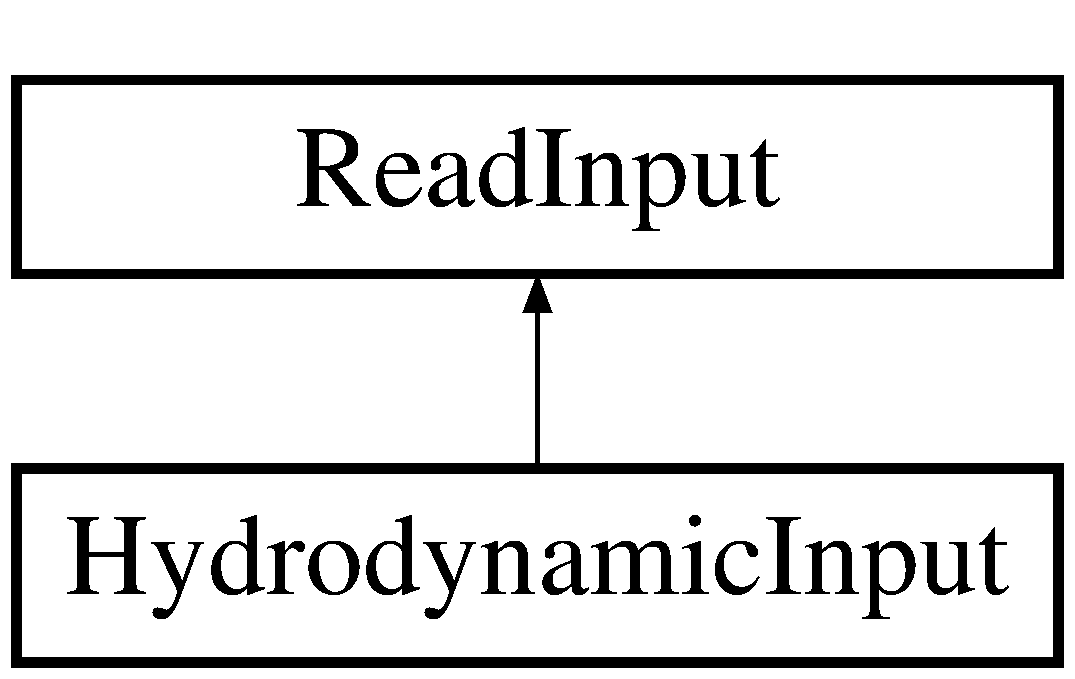
\includegraphics[height=2.000000cm]{class_hydrodynamic_input}
\end{center}
\end{figure}
\subsection*{Protected Member Functions}
\begin{DoxyCompactItemize}
\item 
void \hyperlink{class_hydrodynamic_input_a311ec06f62b7929fb6712e90240a1436}{initialize\-Defaults} ()
\item 
\hypertarget{class_hydrodynamic_input_a5497b513fc1785b84dccea59fd16fff2}{void {\bfseries set\-Data} (istream \&)}\label{class_hydrodynamic_input_a5497b513fc1785b84dccea59fd16fff2}

\item 
int \hyperlink{class_hydrodynamic_input_a6cf4ad1a8407191c8e2633ca0554f641}{legal\-Keyword} (string)
\end{DoxyCompactItemize}
\subsection*{Additional Inherited Members}


\subsection{Member Function Documentation}
\hypertarget{class_hydrodynamic_input_a311ec06f62b7929fb6712e90240a1436}{\index{Hydrodynamic\-Input@{Hydrodynamic\-Input}!initialize\-Defaults@{initialize\-Defaults}}
\index{initialize\-Defaults@{initialize\-Defaults}!HydrodynamicInput@{Hydrodynamic\-Input}}
\subsubsection[{initialize\-Defaults}]{\setlength{\rightskip}{0pt plus 5cm}void Hydrodynamic\-Input\-::initialize\-Defaults (
\begin{DoxyParamCaption}
{}
\end{DoxyParamCaption}
)\hspace{0.3cm}{\ttfamily [protected]}, {\ttfamily [virtual]}}}\label{class_hydrodynamic_input_a311ec06f62b7929fb6712e90240a1436}
Must be implemented by child class. 

Implements \hyperlink{class_read_input_a4ff2727b876cfd7c01299b08bdd65646}{Read\-Input}.

\hypertarget{class_hydrodynamic_input_a6cf4ad1a8407191c8e2633ca0554f641}{\index{Hydrodynamic\-Input@{Hydrodynamic\-Input}!legal\-Keyword@{legal\-Keyword}}
\index{legal\-Keyword@{legal\-Keyword}!HydrodynamicInput@{Hydrodynamic\-Input}}
\subsubsection[{legal\-Keyword}]{\setlength{\rightskip}{0pt plus 5cm}int Hydrodynamic\-Input\-::legal\-Keyword (
\begin{DoxyParamCaption}
\item[{string}]{}
\end{DoxyParamCaption}
)\hspace{0.3cm}{\ttfamily [protected]}, {\ttfamily [virtual]}}}\label{class_hydrodynamic_input_a6cf4ad1a8407191c8e2633ca0554f641}
Must be implemented by child class, determine if keyword is legal. 

Implements \hyperlink{class_read_input_a4c67f10e813686bf635dd4c6bb2c61bc}{Read\-Input}.



The documentation for this class was generated from the following files\-:\begin{DoxyCompactItemize}
\item 
Visual Studio 2010/\-Projects/o\-Freq Windows V\-S2010/o\-Freq/hydrodynamicinput.\-h\item 
Visual Studio 2010/\-Projects/o\-Freq Windows V\-S2010/o\-Freq/hydrodynamicinput.\-cpp\end{DoxyCompactItemize}

\hypertarget{class_motion_model}{\section{Motion\-Model Class Reference}
\label{class_motion_model}\index{Motion\-Model@{Motion\-Model}}
}


{\ttfamily \#include $<$motionmodel.\-h$>$}

\subsection*{Public Member Functions}
\begin{DoxyCompactItemize}
\item 
\hyperlink{class_motion_model_a5a5e4bba0f6ca24e1fdd316458f4f824}{Motion\-Model} ()
\item 
\hyperlink{class_motion_model_ac48a359c77d9efe39d4ec8c9e862a1cd}{$\sim$\-Motion\-Model} ()
\item 
\hyperlink{class_body_with_force_matrix}{Body\-With\-Force\-Matrix} \hyperlink{class_motion_model_ad70067e7f0e5b12978f1dc7f1722c2e1}{set\-Body\-Data} (\hyperlink{class_body}{Body}, \hyperlink{class_user_forces}{User\-Forces})
\item 
void \hyperlink{class_motion_model_ae57d6c22a960aa559bfdc16ca4737a0b}{set\-Wave\-Frequencies} (double)
\end{DoxyCompactItemize}
\subsection*{Static Public Member Functions}
\begin{DoxyCompactItemize}
\item 
static int \hyperlink{class_motion_model_a6eb1d5de348da32ae03936030eba4f2b}{get\-Matrix\-Size} (string)
\end{DoxyCompactItemize}
\subsection*{Public Attributes}
\begin{DoxyCompactItemize}
\item 
double \hyperlink{class_motion_model_af8980ee05f544c75ec1ebe551045c261}{cur\-Wave\-Freq}
\end{DoxyCompactItemize}


\subsection{Detailed Description}
This class holds data for the motion model and calculates the specified equation of motion. 

\subsection{Constructor \& Destructor Documentation}
\hypertarget{class_motion_model_a5a5e4bba0f6ca24e1fdd316458f4f824}{\index{Motion\-Model@{Motion\-Model}!Motion\-Model@{Motion\-Model}}
\index{Motion\-Model@{Motion\-Model}!MotionModel@{Motion\-Model}}
\subsubsection[{Motion\-Model}]{\setlength{\rightskip}{0pt plus 5cm}Motion\-Model\-::\-Motion\-Model (
\begin{DoxyParamCaption}
{}
\end{DoxyParamCaption}
)}}\label{class_motion_model_a5a5e4bba0f6ca24e1fdd316458f4f824}
The default constructor. \hypertarget{class_motion_model_ac48a359c77d9efe39d4ec8c9e862a1cd}{\index{Motion\-Model@{Motion\-Model}!$\sim$\-Motion\-Model@{$\sim$\-Motion\-Model}}
\index{$\sim$\-Motion\-Model@{$\sim$\-Motion\-Model}!MotionModel@{Motion\-Model}}
\subsubsection[{$\sim$\-Motion\-Model}]{\setlength{\rightskip}{0pt plus 5cm}Motion\-Model\-::$\sim$\-Motion\-Model (
\begin{DoxyParamCaption}
{}
\end{DoxyParamCaption}
)}}\label{class_motion_model_ac48a359c77d9efe39d4ec8c9e862a1cd}
The default destructor, nothing happens here. 

\subsection{Member Function Documentation}
\hypertarget{class_motion_model_a6eb1d5de348da32ae03936030eba4f2b}{\index{Motion\-Model@{Motion\-Model}!get\-Matrix\-Size@{get\-Matrix\-Size}}
\index{get\-Matrix\-Size@{get\-Matrix\-Size}!MotionModel@{Motion\-Model}}
\subsubsection[{get\-Matrix\-Size}]{\setlength{\rightskip}{0pt plus 5cm}int Motion\-Model\-::get\-Matrix\-Size (
\begin{DoxyParamCaption}
\item[{string}]{motion\-Type}
\end{DoxyParamCaption}
)\hspace{0.3cm}{\ttfamily [static]}}}\label{class_motion_model_a6eb1d5de348da32ae03936030eba4f2b}
Get the matrix size which depends on which equation of motion is used. 
\begin{DoxyParams}{Parameters}
{\em motion\-Type} & The motion model. \\
\hline
\end{DoxyParams}
\hypertarget{class_motion_model_ad70067e7f0e5b12978f1dc7f1722c2e1}{\index{Motion\-Model@{Motion\-Model}!set\-Body\-Data@{set\-Body\-Data}}
\index{set\-Body\-Data@{set\-Body\-Data}!MotionModel@{Motion\-Model}}
\subsubsection[{set\-Body\-Data}]{\setlength{\rightskip}{0pt plus 5cm}{\bf Body\-With\-Force\-Matrix} Motion\-Model\-::set\-Body\-Data (
\begin{DoxyParamCaption}
\item[{{\bf Body}}]{body\-Data\-In, }
\item[{{\bf User\-Forces}}]{user\-Forces\-In}
\end{DoxyParamCaption}
)}}\label{class_motion_model_ad70067e7f0e5b12978f1dc7f1722c2e1}
Retrieve and calculate the equation of motion body with force matrix object. 
\begin{DoxyParams}{Parameters}
{\em body\-Data\-In} & The body. \\
\hline
{\em user\-Forces\-In} & The User Forces. \\
\hline
\end{DoxyParams}
\begin{DoxyReturn}{Returns}
The \hyperlink{class_body}{Body} with \hyperlink{class_force}{Force} Matrix after specified equation of motion is calculated. 
\end{DoxyReturn}
\hypertarget{class_motion_model_ae57d6c22a960aa559bfdc16ca4737a0b}{\index{Motion\-Model@{Motion\-Model}!set\-Wave\-Frequencies@{set\-Wave\-Frequencies}}
\index{set\-Wave\-Frequencies@{set\-Wave\-Frequencies}!MotionModel@{Motion\-Model}}
\subsubsection[{set\-Wave\-Frequencies}]{\setlength{\rightskip}{0pt plus 5cm}void Motion\-Model\-::set\-Wave\-Frequencies (
\begin{DoxyParamCaption}
\item[{double}]{new\-Wave\-Freq}
\end{DoxyParamCaption}
)}}\label{class_motion_model_ae57d6c22a960aa559bfdc16ca4737a0b}
Set the wave frequencies list. 
\begin{DoxyParams}{Parameters}
{\em new\-Wave\-Freq} & The list of wave frequencies. \\
\hline
\end{DoxyParams}


\subsection{Member Data Documentation}
\hypertarget{class_motion_model_af8980ee05f544c75ec1ebe551045c261}{\index{Motion\-Model@{Motion\-Model}!cur\-Wave\-Freq@{cur\-Wave\-Freq}}
\index{cur\-Wave\-Freq@{cur\-Wave\-Freq}!MotionModel@{Motion\-Model}}
\subsubsection[{cur\-Wave\-Freq}]{\setlength{\rightskip}{0pt plus 5cm}double Motion\-Model\-::cur\-Wave\-Freq}}\label{class_motion_model_af8980ee05f544c75ec1ebe551045c261}
The current wave frequency. 

The documentation for this class was generated from the following files\-:\begin{DoxyCompactItemize}
\item 
Visual Studio 2010/\-Projects/o\-Freq Windows V\-S2010/o\-Freq/motionmodel.\-h\item 
Visual Studio 2010/\-Projects/o\-Freq Windows V\-S2010/o\-Freq/motionmodel.\-cpp\end{DoxyCompactItemize}

\hypertarget{class_motion_solver}{\section{Motion\-Solver Class Reference}
\label{class_motion_solver}\index{Motion\-Solver@{Motion\-Solver}}
}


{\ttfamily \#include $<$motionsolver.\-h$>$}

\subsection*{Public Member Functions}
\begin{DoxyCompactItemize}
\item 
\hyperlink{class_motion_solver_ae231d7c407ef35357e519053091b6003}{Motion\-Solver} (vector$<$ \hyperlink{class_body}{Body} $>$, \hyperlink{class_user_forces}{User\-Forces}, double)
\item 
\hyperlink{class_motion_solver_ae1fb5f389752a21a6d65ce41599b9b91}{$\sim$\-Motion\-Solver} ()
\item 
void \hyperlink{class_motion_solver_ac6c03c2a45d7868b5acb76324fa29279}{set\-Matrix\-Index\-Positions} (int, int)
\item 
vector$<$ cx\-\_\-mat $>$ \hyperlink{class_motion_solver_a89c37a28a333474de2d0d51bada81afa}{sum\-Reactive\-Force\-Each\-Set} (vector$<$ \hyperlink{class_reactive_force_matrix}{Reactive\-Force\-Matrix} $>$)
\item 
cx\-\_\-mat \hyperlink{class_motion_solver_a58ec4344deda599d9b1de11aa3e6abde}{sum\-Active\-Force\-Each\-Set} (vector$<$ cx\-\_\-mat $>$)
\item 
cx\-\_\-mat \hyperlink{class_motion_solver_a26a41ac6907d24228de0a6ddcf9911ce}{sum\-Derivatives} (vector$<$ cx\-\_\-mat $>$)
\item 
vector$<$ cx\-\_\-mat $>$ \hyperlink{class_motion_solver_a2358d623842d0634576d978db98b9198}{Calculate\-Outputs} ()
\end{DoxyCompactItemize}
\subsection*{Public Attributes}
\begin{DoxyCompactItemize}
\item 
vector$<$ \hyperlink{class_body}{Body} $>$ \hyperlink{class_motion_solver_aa706c345b20614a18e9f8f59c6174d2a}{the\-Body\-Data}
\item 
\hyperlink{class_user_forces}{User\-Forces} \hyperlink{class_motion_solver_a9c8dd3a151361ae664c9ff4e9958f649}{the\-Forces\-Data}
\item 
vector$<$ \hyperlink{class_body_with_force_matrix}{Body\-With\-Force\-Matrix} $>$ \hyperlink{class_motion_solver_ac6c73cbeb23091b0064a9a2d0cd0752c}{the\-Body\-With\-Force\-Matrix}
\item 
\hyperlink{class_motion_model}{Motion\-Model} \hyperlink{class_motion_solver_a19e40f754e74afd9f99a3944360165bf}{the\-Motion\-Model}
\item 
double \hyperlink{class_motion_solver_a01ca22785130c0612045094790e2f992}{cur\-Wave\-Frequency}
\item 
int \hyperlink{class_motion_solver_af209f386af69a39839061e436630906c}{max\-Matrix\-Size}
\item 
cx\-\_\-mat \hyperlink{class_motion_solver_a29bb1f9a2fd145b4e8fc74ad711e4351}{reactive\-Force\-Matrix\-Global}
\item 
cx\-\_\-mat \hyperlink{class_motion_solver_a800bc918ff0075782368046bd51eeb87}{active\-Force\-Matrix\-Global}
\item 
cx\-\_\-mat \hyperlink{class_motion_solver_aba617c457e3dab115693c4b3a23f9827}{solution\-Column\-Matrix}
\end{DoxyCompactItemize}


\subsection{Detailed Description}
This class holds data for the motion solver and performs calculations on all of the data to get the solution matrix. 

\subsection{Constructor \& Destructor Documentation}
\hypertarget{class_motion_solver_ae231d7c407ef35357e519053091b6003}{\index{Motion\-Solver@{Motion\-Solver}!Motion\-Solver@{Motion\-Solver}}
\index{Motion\-Solver@{Motion\-Solver}!MotionSolver@{Motion\-Solver}}
\subsubsection[{Motion\-Solver}]{\setlength{\rightskip}{0pt plus 5cm}Motion\-Solver\-::\-Motion\-Solver (
\begin{DoxyParamCaption}
\item[{vector$<$ {\bf Body} $>$}]{body\-Data\-In, }
\item[{{\bf User\-Forces}}]{user\-Forces\-In, }
\item[{double}]{new\-Wave\-Freq}
\end{DoxyParamCaption}
)}}\label{class_motion_solver_ae231d7c407ef35357e519053091b6003}
The constructor. 
\begin{DoxyParams}{Parameters}
{\em body\-Data\-In} & The body. \\
\hline
{\em user\-Forces\-In} & The User Forces. \\
\hline
{\em new\-Wave\-Freq} & The wave frequencies. \\
\hline
\end{DoxyParams}
\hypertarget{class_motion_solver_ae1fb5f389752a21a6d65ce41599b9b91}{\index{Motion\-Solver@{Motion\-Solver}!$\sim$\-Motion\-Solver@{$\sim$\-Motion\-Solver}}
\index{$\sim$\-Motion\-Solver@{$\sim$\-Motion\-Solver}!MotionSolver@{Motion\-Solver}}
\subsubsection[{$\sim$\-Motion\-Solver}]{\setlength{\rightskip}{0pt plus 5cm}Motion\-Solver\-::$\sim$\-Motion\-Solver (
\begin{DoxyParamCaption}
{}
\end{DoxyParamCaption}
)}}\label{class_motion_solver_ae1fb5f389752a21a6d65ce41599b9b91}
The default destructor, nothing happens here. 

\subsection{Member Function Documentation}
\hypertarget{class_motion_solver_a2358d623842d0634576d978db98b9198}{\index{Motion\-Solver@{Motion\-Solver}!Calculate\-Outputs@{Calculate\-Outputs}}
\index{Calculate\-Outputs@{Calculate\-Outputs}!MotionSolver@{Motion\-Solver}}
\subsubsection[{Calculate\-Outputs}]{\setlength{\rightskip}{0pt plus 5cm}vector$<$ cx\-\_\-mat $>$ Motion\-Solver\-::\-Calculate\-Outputs (
\begin{DoxyParamCaption}
{}
\end{DoxyParamCaption}
)}}\label{class_motion_solver_a2358d623842d0634576d978db98b9198}
Calculate the Solution and return the solutions for each body. \begin{DoxyReturn}{Returns}
A list of solutions for each body. 
\end{DoxyReturn}
\hypertarget{class_motion_solver_ac6c03c2a45d7868b5acb76324fa29279}{\index{Motion\-Solver@{Motion\-Solver}!set\-Matrix\-Index\-Positions@{set\-Matrix\-Index\-Positions}}
\index{set\-Matrix\-Index\-Positions@{set\-Matrix\-Index\-Positions}!MotionSolver@{Motion\-Solver}}
\subsubsection[{set\-Matrix\-Index\-Positions}]{\setlength{\rightskip}{0pt plus 5cm}void Motion\-Solver\-::set\-Matrix\-Index\-Positions (
\begin{DoxyParamCaption}
\item[{int}]{num\-Bodies, }
\item[{int}]{per\-Matrix\-Size}
\end{DoxyParamCaption}
)}}\label{class_motion_solver_ac6c03c2a45d7868b5acb76324fa29279}
Set the matrix index positions in the reactive force matrix. 
\begin{DoxyParams}{Parameters}
{\em num\-Bodies} & The number of bodies. \\
\hline
{\em per\-Matrix\-Size} & The roww/column length of matrix. \\
\hline
\end{DoxyParams}
\hypertarget{class_motion_solver_a58ec4344deda599d9b1de11aa3e6abde}{\index{Motion\-Solver@{Motion\-Solver}!sum\-Active\-Force\-Each\-Set@{sum\-Active\-Force\-Each\-Set}}
\index{sum\-Active\-Force\-Each\-Set@{sum\-Active\-Force\-Each\-Set}!MotionSolver@{Motion\-Solver}}
\subsubsection[{sum\-Active\-Force\-Each\-Set}]{\setlength{\rightskip}{0pt plus 5cm}cx\-\_\-mat Motion\-Solver\-::sum\-Active\-Force\-Each\-Set (
\begin{DoxyParamCaption}
\item[{vector$<$ cx\-\_\-mat $>$}]{the\-Active\-Force\-Matrix}
\end{DoxyParamCaption}
)}}\label{class_motion_solver_a58ec4344deda599d9b1de11aa3e6abde}
Sum active forces for each set. 
\begin{DoxyParams}{Parameters}
{\em the\-Active\-Force\-Matrix} & The active force matrix. \\
\hline
\end{DoxyParams}
\begin{DoxyReturn}{Returns}
The sum of active force matrix. 
\end{DoxyReturn}
\hypertarget{class_motion_solver_a26a41ac6907d24228de0a6ddcf9911ce}{\index{Motion\-Solver@{Motion\-Solver}!sum\-Derivatives@{sum\-Derivatives}}
\index{sum\-Derivatives@{sum\-Derivatives}!MotionSolver@{Motion\-Solver}}
\subsubsection[{sum\-Derivatives}]{\setlength{\rightskip}{0pt plus 5cm}cx\-\_\-mat Motion\-Solver\-::sum\-Derivatives (
\begin{DoxyParamCaption}
\item[{vector$<$ cx\-\_\-mat $>$}]{the\-Reactive\-Force\-Matrix}
\end{DoxyParamCaption}
)}}\label{class_motion_solver_a26a41ac6907d24228de0a6ddcf9911ce}
Sum Derivatives for reactive force matrix. 
\begin{DoxyParams}{Parameters}
{\em the\-Reactive\-Force\-Matrix} & The reactive force matrix. \\
\hline
\end{DoxyParams}
\begin{DoxyReturn}{Returns}
T\-Single matrix that is the sum of Matrices passed in. 
\end{DoxyReturn}
\hypertarget{class_motion_solver_a89c37a28a333474de2d0d51bada81afa}{\index{Motion\-Solver@{Motion\-Solver}!sum\-Reactive\-Force\-Each\-Set@{sum\-Reactive\-Force\-Each\-Set}}
\index{sum\-Reactive\-Force\-Each\-Set@{sum\-Reactive\-Force\-Each\-Set}!MotionSolver@{Motion\-Solver}}
\subsubsection[{sum\-Reactive\-Force\-Each\-Set}]{\setlength{\rightskip}{0pt plus 5cm}vector$<$ cx\-\_\-mat $>$ Motion\-Solver\-::sum\-Reactive\-Force\-Each\-Set (
\begin{DoxyParamCaption}
\item[{vector$<$ {\bf Reactive\-Force\-Matrix} $>$}]{the\-Reactive\-Force\-Matrix}
\end{DoxyParamCaption}
)}}\label{class_motion_solver_a89c37a28a333474de2d0d51bada81afa}
Sum Reactive forces for each set. 
\begin{DoxyParams}{Parameters}
{\em the\-Reactive\-Force\-Matrix} & The Reactive force matrix. \\
\hline
\end{DoxyParams}
\begin{DoxyReturn}{Returns}
The sum of reactive force matrices. 
\end{DoxyReturn}


\subsection{Member Data Documentation}
\hypertarget{class_motion_solver_a800bc918ff0075782368046bd51eeb87}{\index{Motion\-Solver@{Motion\-Solver}!active\-Force\-Matrix\-Global@{active\-Force\-Matrix\-Global}}
\index{active\-Force\-Matrix\-Global@{active\-Force\-Matrix\-Global}!MotionSolver@{Motion\-Solver}}
\subsubsection[{active\-Force\-Matrix\-Global}]{\setlength{\rightskip}{0pt plus 5cm}cx\-\_\-mat Motion\-Solver\-::active\-Force\-Matrix\-Global}}\label{class_motion_solver_a800bc918ff0075782368046bd51eeb87}
F Matrix (Active \hyperlink{class_force}{Force} Matirx Global) \hypertarget{class_motion_solver_a01ca22785130c0612045094790e2f992}{\index{Motion\-Solver@{Motion\-Solver}!cur\-Wave\-Frequency@{cur\-Wave\-Frequency}}
\index{cur\-Wave\-Frequency@{cur\-Wave\-Frequency}!MotionSolver@{Motion\-Solver}}
\subsubsection[{cur\-Wave\-Frequency}]{\setlength{\rightskip}{0pt plus 5cm}double Motion\-Solver\-::cur\-Wave\-Frequency}}\label{class_motion_solver_a01ca22785130c0612045094790e2f992}
The current wave frequency \hypertarget{class_motion_solver_af209f386af69a39839061e436630906c}{\index{Motion\-Solver@{Motion\-Solver}!max\-Matrix\-Size@{max\-Matrix\-Size}}
\index{max\-Matrix\-Size@{max\-Matrix\-Size}!MotionSolver@{Motion\-Solver}}
\subsubsection[{max\-Matrix\-Size}]{\setlength{\rightskip}{0pt plus 5cm}int Motion\-Solver\-::max\-Matrix\-Size}}\label{class_motion_solver_af209f386af69a39839061e436630906c}
The max row/column size of the matrix \hypertarget{class_motion_solver_a29bb1f9a2fd145b4e8fc74ad711e4351}{\index{Motion\-Solver@{Motion\-Solver}!reactive\-Force\-Matrix\-Global@{reactive\-Force\-Matrix\-Global}}
\index{reactive\-Force\-Matrix\-Global@{reactive\-Force\-Matrix\-Global}!MotionSolver@{Motion\-Solver}}
\subsubsection[{reactive\-Force\-Matrix\-Global}]{\setlength{\rightskip}{0pt plus 5cm}cx\-\_\-mat Motion\-Solver\-::reactive\-Force\-Matrix\-Global}}\label{class_motion_solver_a29bb1f9a2fd145b4e8fc74ad711e4351}
A Matrix (Reactive \hyperlink{class_force}{Force} Matrix Global) \hypertarget{class_motion_solver_aba617c457e3dab115693c4b3a23f9827}{\index{Motion\-Solver@{Motion\-Solver}!solution\-Column\-Matrix@{solution\-Column\-Matrix}}
\index{solution\-Column\-Matrix@{solution\-Column\-Matrix}!MotionSolver@{Motion\-Solver}}
\subsubsection[{solution\-Column\-Matrix}]{\setlength{\rightskip}{0pt plus 5cm}cx\-\_\-mat Motion\-Solver\-::solution\-Column\-Matrix}}\label{class_motion_solver_aba617c457e3dab115693c4b3a23f9827}
X Matrix (Solution Column Matrix) \hypertarget{class_motion_solver_aa706c345b20614a18e9f8f59c6174d2a}{\index{Motion\-Solver@{Motion\-Solver}!the\-Body\-Data@{the\-Body\-Data}}
\index{the\-Body\-Data@{the\-Body\-Data}!MotionSolver@{Motion\-Solver}}
\subsubsection[{the\-Body\-Data}]{\setlength{\rightskip}{0pt plus 5cm}vector$<${\bf Body}$>$ Motion\-Solver\-::the\-Body\-Data}}\label{class_motion_solver_aa706c345b20614a18e9f8f59c6174d2a}
original body data from input files \hypertarget{class_motion_solver_ac6c73cbeb23091b0064a9a2d0cd0752c}{\index{Motion\-Solver@{Motion\-Solver}!the\-Body\-With\-Force\-Matrix@{the\-Body\-With\-Force\-Matrix}}
\index{the\-Body\-With\-Force\-Matrix@{the\-Body\-With\-Force\-Matrix}!MotionSolver@{Motion\-Solver}}
\subsubsection[{the\-Body\-With\-Force\-Matrix}]{\setlength{\rightskip}{0pt plus 5cm}vector$<${\bf Body\-With\-Force\-Matrix}$>$ Motion\-Solver\-::the\-Body\-With\-Force\-Matrix}}\label{class_motion_solver_ac6c73cbeb23091b0064a9a2d0cd0752c}
\hyperlink{class_body}{Body} with \hyperlink{class_force}{Force} Coefficients \hypertarget{class_motion_solver_a9c8dd3a151361ae664c9ff4e9958f649}{\index{Motion\-Solver@{Motion\-Solver}!the\-Forces\-Data@{the\-Forces\-Data}}
\index{the\-Forces\-Data@{the\-Forces\-Data}!MotionSolver@{Motion\-Solver}}
\subsubsection[{the\-Forces\-Data}]{\setlength{\rightskip}{0pt plus 5cm}{\bf User\-Forces} Motion\-Solver\-::the\-Forces\-Data}}\label{class_motion_solver_a9c8dd3a151361ae664c9ff4e9958f649}
original force data from input files \hypertarget{class_motion_solver_a19e40f754e74afd9f99a3944360165bf}{\index{Motion\-Solver@{Motion\-Solver}!the\-Motion\-Model@{the\-Motion\-Model}}
\index{the\-Motion\-Model@{the\-Motion\-Model}!MotionSolver@{Motion\-Solver}}
\subsubsection[{the\-Motion\-Model}]{\setlength{\rightskip}{0pt plus 5cm}{\bf Motion\-Model} Motion\-Solver\-::the\-Motion\-Model}}\label{class_motion_solver_a19e40f754e74afd9f99a3944360165bf}
The motion model. 

The documentation for this class was generated from the following files\-:\begin{DoxyCompactItemize}
\item 
Visual Studio 2010/\-Projects/o\-Freq Windows V\-S2010/o\-Freq/motionsolver.\-h\item 
Visual Studio 2010/\-Projects/o\-Freq Windows V\-S2010/o\-Freq/motionsolver.\-cpp\end{DoxyCompactItemize}

\hypertarget{class_output_derived}{\section{Output\-Derived Class Reference}
\label{class_output_derived}\index{Output\-Derived@{Output\-Derived}}
}


{\ttfamily \#include $<$outputderived.\-h$>$}

Inheritance diagram for Output\-Derived\-:\begin{figure}[H]
\begin{center}
\leavevmode
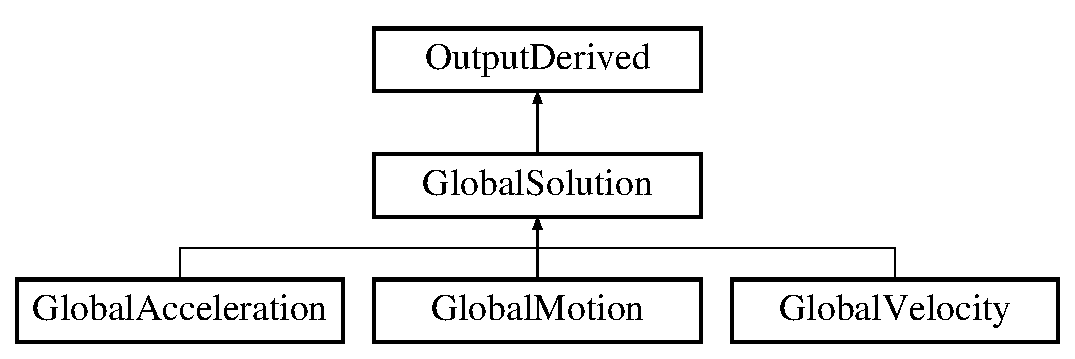
\includegraphics[height=3.000000cm]{class_output_derived}
\end{center}
\end{figure}
\subsection*{Public Member Functions}
\begin{DoxyCompactItemize}
\item 
\hyperlink{class_output_derived_af8b70b70b8a5089f2b673da8b59a7b6a}{Output\-Derived} ()
\item 
\hyperlink{class_output_derived_a4dde733443e52964c74d8bb6477f85f7}{$\sim$\-Output\-Derived} ()
\item 
virtual cx\-\_\-mat \hyperlink{class_output_derived_a1e0052dd24822806481976e42a2f5f30}{calculate\-Output} (cx\-\_\-mat, double)=0
\end{DoxyCompactItemize}
\subsection*{Public Attributes}
\begin{DoxyCompactItemize}
\item 
\hyperlink{class_body}{Body} \hyperlink{class_output_derived_aa326f34bcce8fa06e67016bb57069e16}{the\-Body}
\item 
int \hyperlink{class_output_derived_af0bf64d22f81f60368cd01a448596fe9}{cur\-Wave\-Direction}
\item 
string \hyperlink{class_output_derived_ae2ee713862294ab274c78a604ee962b4}{name}
\end{DoxyCompactItemize}


\subsection{Detailed Description}
This abstract class represents the Derived Outputs. 

\subsection{Constructor \& Destructor Documentation}
\hypertarget{class_output_derived_af8b70b70b8a5089f2b673da8b59a7b6a}{\index{Output\-Derived@{Output\-Derived}!Output\-Derived@{Output\-Derived}}
\index{Output\-Derived@{Output\-Derived}!OutputDerived@{Output\-Derived}}
\subsubsection[{Output\-Derived}]{\setlength{\rightskip}{0pt plus 5cm}Output\-Derived\-::\-Output\-Derived (
\begin{DoxyParamCaption}
\item[{void}]{}
\end{DoxyParamCaption}
)}}\label{class_output_derived_af8b70b70b8a5089f2b673da8b59a7b6a}
This default constructor creates a Output Derived object. \hypertarget{class_output_derived_a4dde733443e52964c74d8bb6477f85f7}{\index{Output\-Derived@{Output\-Derived}!$\sim$\-Output\-Derived@{$\sim$\-Output\-Derived}}
\index{$\sim$\-Output\-Derived@{$\sim$\-Output\-Derived}!OutputDerived@{Output\-Derived}}
\subsubsection[{$\sim$\-Output\-Derived}]{\setlength{\rightskip}{0pt plus 5cm}Output\-Derived\-::$\sim$\-Output\-Derived (
\begin{DoxyParamCaption}
\item[{void}]{}
\end{DoxyParamCaption}
)}}\label{class_output_derived_a4dde733443e52964c74d8bb6477f85f7}
The default destructor, nothing happens here. 

\subsection{Member Function Documentation}
\hypertarget{class_output_derived_a1e0052dd24822806481976e42a2f5f30}{\index{Output\-Derived@{Output\-Derived}!calculate\-Output@{calculate\-Output}}
\index{calculate\-Output@{calculate\-Output}!OutputDerived@{Output\-Derived}}
\subsubsection[{calculate\-Output}]{\setlength{\rightskip}{0pt plus 5cm}virtual cx\-\_\-mat Output\-Derived\-::calculate\-Output (
\begin{DoxyParamCaption}
\item[{cx\-\_\-mat}]{, }
\item[{double}]{}
\end{DoxyParamCaption}
)\hspace{0.3cm}{\ttfamily [pure virtual]}}}\label{class_output_derived_a1e0052dd24822806481976e42a2f5f30}
Child class mus implement \char`\"{}\-Calculates the outputs\char`\"{}. 
\begin{DoxyParams}{Parameters}
{\em matrix\-In} & The original Matrix that is used for calculations. \\
\hline
{\em cur\-Wave\-Freq} & The current wave frequency. \\
\hline
\end{DoxyParams}
\begin{DoxyReturn}{Returns}
The new matrix with calculations on each index. 
\end{DoxyReturn}


Implemented in \hyperlink{class_global_solution_a15634073f63559cbfd65b32b79cd7fbd}{Global\-Solution}.



\subsection{Member Data Documentation}
\hypertarget{class_output_derived_af0bf64d22f81f60368cd01a448596fe9}{\index{Output\-Derived@{Output\-Derived}!cur\-Wave\-Direction@{cur\-Wave\-Direction}}
\index{cur\-Wave\-Direction@{cur\-Wave\-Direction}!OutputDerived@{Output\-Derived}}
\subsubsection[{cur\-Wave\-Direction}]{\setlength{\rightskip}{0pt plus 5cm}int Output\-Derived\-::cur\-Wave\-Direction}}\label{class_output_derived_af0bf64d22f81f60368cd01a448596fe9}
The current wave direction. \hypertarget{class_output_derived_ae2ee713862294ab274c78a604ee962b4}{\index{Output\-Derived@{Output\-Derived}!name@{name}}
\index{name@{name}!OutputDerived@{Output\-Derived}}
\subsubsection[{name}]{\setlength{\rightskip}{0pt plus 5cm}string Output\-Derived\-::name}}\label{class_output_derived_ae2ee713862294ab274c78a604ee962b4}
The name.?? N\-E\-E\-D\-S T\-O B\-E F\-I\-X\-E\-D \hypertarget{class_output_derived_aa326f34bcce8fa06e67016bb57069e16}{\index{Output\-Derived@{Output\-Derived}!the\-Body@{the\-Body}}
\index{the\-Body@{the\-Body}!OutputDerived@{Output\-Derived}}
\subsubsection[{the\-Body}]{\setlength{\rightskip}{0pt plus 5cm}{\bf Body} Output\-Derived\-::the\-Body}}\label{class_output_derived_aa326f34bcce8fa06e67016bb57069e16}
Holds a reference to the body for outputs. 

The documentation for this class was generated from the following files\-:\begin{DoxyCompactItemize}
\item 
Visual Studio 2010/\-Projects/o\-Freq Windows V\-S2010/o\-Freq/outputderived.\-h\item 
Visual Studio 2010/\-Projects/o\-Freq Windows V\-S2010/o\-Freq/outputderived.\-cpp\end{DoxyCompactItemize}

\hypertarget{class_outputs_body}{\section{Outputs\-Body Class Reference}
\label{class_outputs_body}\index{Outputs\-Body@{Outputs\-Body}}
}


{\ttfamily \#include $<$outputsbody.\-h$>$}

\subsection*{Public Member Functions}
\begin{DoxyCompactItemize}
\item 
\hyperlink{class_outputs_body_a0eac4499cabfe665627c5ae248d716fb}{Outputs\-Body} (\hyperlink{class_body_with_solution}{Body\-With\-Solution}, vector$<$ double $>$)
\item 
\hyperlink{class_outputs_body_a9ec0c3721f511168c425b792bdaf2d62}{$\sim$\-Outputs\-Body} ()
\item 
vector$<$ cx\-\_\-mat $>$ \hyperlink{class_outputs_body_a648ab9c3d60a0570d20265ec3a8a7e74}{get\-Output\-Type} (int)
\item 
vector$<$ cx\-\_\-mat $>$ \hyperlink{class_outputs_body_ad3930dfef26bd650ab09c8f0e05315b3}{get\-Output\-List} ()
\item 
void \hyperlink{class_outputs_body_a410ed10a395c4d1a598edfdd0f791e0a}{calculate\-Outputs} ()
\end{DoxyCompactItemize}
\subsection*{Public Attributes}
\begin{DoxyCompactItemize}
\item 
\hyperlink{class_body_with_solution}{Body\-With\-Solution} \hyperlink{class_outputs_body_aa03c8f557f55a5e8b806f4fc62397198}{the\-Body}
\item 
vector$<$ double $>$ \hyperlink{class_outputs_body_a625ad12a75ab02375ec369c47bfa4b52}{frequencies}
\end{DoxyCompactItemize}


\subsection{Detailed Description}
This class holds the global solutions for all frequncies for a single body object. 

\subsection{Constructor \& Destructor Documentation}
\hypertarget{class_outputs_body_a0eac4499cabfe665627c5ae248d716fb}{\index{Outputs\-Body@{Outputs\-Body}!Outputs\-Body@{Outputs\-Body}}
\index{Outputs\-Body@{Outputs\-Body}!OutputsBody@{Outputs\-Body}}
\subsubsection[{Outputs\-Body}]{\setlength{\rightskip}{0pt plus 5cm}Outputs\-Body\-::\-Outputs\-Body (
\begin{DoxyParamCaption}
\item[{{\bf Body\-With\-Solution}}]{body\-In, }
\item[{vector$<$ double $>$}]{frequencies\-In}
\end{DoxyParamCaption}
)}}\label{class_outputs_body_a0eac4499cabfe665627c5ae248d716fb}
Constructor Creates a new Outputs\-Body\-Object and sets the \hyperlink{class_body_with_solution}{Body\-With\-Solution} and wave\-Frequencies. 
\begin{DoxyParams}{Parameters}
{\em body\-In} & Sets Body\-With\-Solution\-Object. \\
\hline
{\em Sets} & the List of wave frequencies. \\
\hline
\end{DoxyParams}
\hypertarget{class_outputs_body_a9ec0c3721f511168c425b792bdaf2d62}{\index{Outputs\-Body@{Outputs\-Body}!$\sim$\-Outputs\-Body@{$\sim$\-Outputs\-Body}}
\index{$\sim$\-Outputs\-Body@{$\sim$\-Outputs\-Body}!OutputsBody@{Outputs\-Body}}
\subsubsection[{$\sim$\-Outputs\-Body}]{\setlength{\rightskip}{0pt plus 5cm}Outputs\-Body\-::$\sim$\-Outputs\-Body (
\begin{DoxyParamCaption}
{}
\end{DoxyParamCaption}
)}}\label{class_outputs_body_a9ec0c3721f511168c425b792bdaf2d62}
The default destructor, nothing happens here. 

\subsection{Member Function Documentation}
\hypertarget{class_outputs_body_a410ed10a395c4d1a598edfdd0f791e0a}{\index{Outputs\-Body@{Outputs\-Body}!calculate\-Outputs@{calculate\-Outputs}}
\index{calculate\-Outputs@{calculate\-Outputs}!OutputsBody@{Outputs\-Body}}
\subsubsection[{calculate\-Outputs}]{\setlength{\rightskip}{0pt plus 5cm}void Outputs\-Body\-::calculate\-Outputs (
\begin{DoxyParamCaption}
{}
\end{DoxyParamCaption}
)}}\label{class_outputs_body_a410ed10a395c4d1a598edfdd0f791e0a}
Calculate S\-Olutions for eahc class type and frequency \hypertarget{class_outputs_body_ad3930dfef26bd650ab09c8f0e05315b3}{\index{Outputs\-Body@{Outputs\-Body}!get\-Output\-List@{get\-Output\-List}}
\index{get\-Output\-List@{get\-Output\-List}!OutputsBody@{Outputs\-Body}}
\subsubsection[{get\-Output\-List}]{\setlength{\rightskip}{0pt plus 5cm}vector$<$ cx\-\_\-mat $>$ Outputs\-Body\-::get\-Output\-List (
\begin{DoxyParamCaption}
{}
\end{DoxyParamCaption}
)}}\label{class_outputs_body_ad3930dfef26bd650ab09c8f0e05315b3}
Retrieve a matrix of all types of Global Solution types. \begin{DoxyReturn}{Returns}
Matrix that has all Global solution types, each column is seperate class type, each index seperate frequency. 
\end{DoxyReturn}
\hypertarget{class_outputs_body_a648ab9c3d60a0570d20265ec3a8a7e74}{\index{Outputs\-Body@{Outputs\-Body}!get\-Output\-Type@{get\-Output\-Type}}
\index{get\-Output\-Type@{get\-Output\-Type}!OutputsBody@{Outputs\-Body}}
\subsubsection[{get\-Output\-Type}]{\setlength{\rightskip}{0pt plus 5cm}vector$<$ cx\-\_\-mat $>$ Outputs\-Body\-::get\-Output\-Type (
\begin{DoxyParamCaption}
\item[{int}]{class\-Type}
\end{DoxyParamCaption}
)}}\label{class_outputs_body_a648ab9c3d60a0570d20265ec3a8a7e74}
Retrieve a matrix of only one type of Global Solution. 
\begin{DoxyParams}{Parameters}
{\em classype} & This specifies the index used to retrieve one of the Global Solutions. \\
\hline
\end{DoxyParams}
\begin{DoxyReturn}{Returns}
Matrix of one type Global Solutions, each index represents different frquency. 
\end{DoxyReturn}


\subsection{Member Data Documentation}
\hypertarget{class_outputs_body_a625ad12a75ab02375ec369c47bfa4b52}{\index{Outputs\-Body@{Outputs\-Body}!frequencies@{frequencies}}
\index{frequencies@{frequencies}!OutputsBody@{Outputs\-Body}}
\subsubsection[{frequencies}]{\setlength{\rightskip}{0pt plus 5cm}vector$<$double$>$ Outputs\-Body\-::frequencies}}\label{class_outputs_body_a625ad12a75ab02375ec369c47bfa4b52}
The list of wave frequencies to be used. \hypertarget{class_outputs_body_aa03c8f557f55a5e8b806f4fc62397198}{\index{Outputs\-Body@{Outputs\-Body}!the\-Body@{the\-Body}}
\index{the\-Body@{the\-Body}!OutputsBody@{Outputs\-Body}}
\subsubsection[{the\-Body}]{\setlength{\rightskip}{0pt plus 5cm}{\bf Body\-With\-Solution} Outputs\-Body\-::the\-Body}}\label{class_outputs_body_aa03c8f557f55a5e8b806f4fc62397198}
Holds object that has body name and solutions. 

The documentation for this class was generated from the following files\-:\begin{DoxyCompactItemize}
\item 
Visual Studio 2010/\-Projects/o\-Freq Windows V\-S2010/o\-Freq/outputsbody.\-h\item 
Visual Studio 2010/\-Projects/o\-Freq Windows V\-S2010/o\-Freq/outputsbody.\-cpp\end{DoxyCompactItemize}

\hypertarget{class_outputs_list}{\section{Outputs\-List Class Reference}
\label{class_outputs_list}\index{Outputs\-List@{Outputs\-List}}
}


{\ttfamily \#include $<$outputslist.\-h$>$}

\subsection*{Public Member Functions}
\begin{DoxyCompactItemize}
\item 
\hyperlink{class_outputs_list_a5f3ea650f5c9ae5e29ad34f2d051e915}{Outputs\-List} ()
\item 
\hyperlink{class_outputs_list_a3a7ab0f85a9874b5563ad3a650219429}{Outputs\-List} (vector$<$ \hyperlink{class_body_with_solution}{Body\-With\-Solution} $>$, vector$<$ double $>$, vector$<$ double $>$)
\item 
\hyperlink{class_outputs_list_ae3e4bc9bece0fd81594fd42576831c0b}{$\sim$\-Outputs\-List} ()
\item 
void \hyperlink{class_outputs_list_a31dd7270ed3468e78168bb1bf85fd79d}{calculate\-Outputs} ()
\end{DoxyCompactItemize}
\subsection*{Public Attributes}
\begin{DoxyCompactItemize}
\item 
vector$<$ \hyperlink{class_outputs_body}{Outputs\-Body} $>$ \hyperlink{class_outputs_list_a060736f6168b7a7ff22480c59ab1cae1}{the\-Outputs\-Body\-List}
\item 
vector$<$ \hyperlink{class_body_with_solution}{Body\-With\-Solution} $>$ \hyperlink{class_outputs_list_a641a2087534a39ba07e5dcc373c3e993}{the\-Body\-List}
\item 
vector$<$ double $>$ \hyperlink{class_outputs_list_afb577c627b76bd4734a450af611313e7}{the\-Frequency\-List}
\item 
vector$<$ double $>$ \hyperlink{class_outputs_list_a2378aea897a70d83842b4aabe3d3c3c2}{the\-Direction\-List}
\end{DoxyCompactItemize}


\subsection{Detailed Description}
This class holds the global solutions for all frequncies for all body object(s). 

\subsection{Constructor \& Destructor Documentation}
\hypertarget{class_outputs_list_a5f3ea650f5c9ae5e29ad34f2d051e915}{\index{Outputs\-List@{Outputs\-List}!Outputs\-List@{Outputs\-List}}
\index{Outputs\-List@{Outputs\-List}!OutputsList@{Outputs\-List}}
\subsubsection[{Outputs\-List}]{\setlength{\rightskip}{0pt plus 5cm}Outputs\-List\-::\-Outputs\-List (
\begin{DoxyParamCaption}
{}
\end{DoxyParamCaption}
)}}\label{class_outputs_list_a5f3ea650f5c9ae5e29ad34f2d051e915}
This default constructor creates a \hyperlink{class_outputs_list}{Outputs\-List} object. \hypertarget{class_outputs_list_a3a7ab0f85a9874b5563ad3a650219429}{\index{Outputs\-List@{Outputs\-List}!Outputs\-List@{Outputs\-List}}
\index{Outputs\-List@{Outputs\-List}!OutputsList@{Outputs\-List}}
\subsubsection[{Outputs\-List}]{\setlength{\rightskip}{0pt plus 5cm}Outputs\-List\-::\-Outputs\-List (
\begin{DoxyParamCaption}
\item[{vector$<$ {\bf Body\-With\-Solution} $>$}]{body\-In, }
\item[{vector$<$ double $>$}]{directions\-In, }
\item[{vector$<$ double $>$}]{frequencies\-In}
\end{DoxyParamCaption}
)}}\label{class_outputs_list_a3a7ab0f85a9874b5563ad3a650219429}
Overloaded constructor 
\begin{DoxyParams}{Parameters}
{\em the\-Body\-List\-In} & All bodies with calculated solutions. \\
\hline
{\em direction\-In} & List of all wave directions. \\
\hline
{\em frequencies\-In} & List of all frequencies. \\
\hline
\end{DoxyParams}
\hypertarget{class_outputs_list_ae3e4bc9bece0fd81594fd42576831c0b}{\index{Outputs\-List@{Outputs\-List}!$\sim$\-Outputs\-List@{$\sim$\-Outputs\-List}}
\index{$\sim$\-Outputs\-List@{$\sim$\-Outputs\-List}!OutputsList@{Outputs\-List}}
\subsubsection[{$\sim$\-Outputs\-List}]{\setlength{\rightskip}{0pt plus 5cm}Outputs\-List\-::$\sim$\-Outputs\-List (
\begin{DoxyParamCaption}
{}
\end{DoxyParamCaption}
)}}\label{class_outputs_list_ae3e4bc9bece0fd81594fd42576831c0b}
The default destructor, nothing happens here. 

\subsection{Member Function Documentation}
\hypertarget{class_outputs_list_a31dd7270ed3468e78168bb1bf85fd79d}{\index{Outputs\-List@{Outputs\-List}!calculate\-Outputs@{calculate\-Outputs}}
\index{calculate\-Outputs@{calculate\-Outputs}!OutputsList@{Outputs\-List}}
\subsubsection[{calculate\-Outputs}]{\setlength{\rightskip}{0pt plus 5cm}void Outputs\-List\-::calculate\-Outputs (
\begin{DoxyParamCaption}
{}
\end{DoxyParamCaption}
)}}\label{class_outputs_list_a31dd7270ed3468e78168bb1bf85fd79d}
Calculate the Global Solutions for each body 

\subsection{Member Data Documentation}
\hypertarget{class_outputs_list_a641a2087534a39ba07e5dcc373c3e993}{\index{Outputs\-List@{Outputs\-List}!the\-Body\-List@{the\-Body\-List}}
\index{the\-Body\-List@{the\-Body\-List}!OutputsList@{Outputs\-List}}
\subsubsection[{the\-Body\-List}]{\setlength{\rightskip}{0pt plus 5cm}vector$<${\bf Body\-With\-Solution}$>$ Outputs\-List\-::the\-Body\-List}}\label{class_outputs_list_a641a2087534a39ba07e5dcc373c3e993}
List of all bodies with soluions computed by motion solver \hypertarget{class_outputs_list_a2378aea897a70d83842b4aabe3d3c3c2}{\index{Outputs\-List@{Outputs\-List}!the\-Direction\-List@{the\-Direction\-List}}
\index{the\-Direction\-List@{the\-Direction\-List}!OutputsList@{Outputs\-List}}
\subsubsection[{the\-Direction\-List}]{\setlength{\rightskip}{0pt plus 5cm}vector$<$double$>$ Outputs\-List\-::the\-Direction\-List}}\label{class_outputs_list_a2378aea897a70d83842b4aabe3d3c3c2}
List of directions used. \hypertarget{class_outputs_list_afb577c627b76bd4734a450af611313e7}{\index{Outputs\-List@{Outputs\-List}!the\-Frequency\-List@{the\-Frequency\-List}}
\index{the\-Frequency\-List@{the\-Frequency\-List}!OutputsList@{Outputs\-List}}
\subsubsection[{the\-Frequency\-List}]{\setlength{\rightskip}{0pt plus 5cm}vector$<$double$>$ Outputs\-List\-::the\-Frequency\-List}}\label{class_outputs_list_afb577c627b76bd4734a450af611313e7}
List of frequencies used. \hypertarget{class_outputs_list_a060736f6168b7a7ff22480c59ab1cae1}{\index{Outputs\-List@{Outputs\-List}!the\-Outputs\-Body\-List@{the\-Outputs\-Body\-List}}
\index{the\-Outputs\-Body\-List@{the\-Outputs\-Body\-List}!OutputsList@{Outputs\-List}}
\subsubsection[{the\-Outputs\-Body\-List}]{\setlength{\rightskip}{0pt plus 5cm}vector$<${\bf Outputs\-Body}$>$ Outputs\-List\-::the\-Outputs\-Body\-List}}\label{class_outputs_list_a060736f6168b7a7ff22480c59ab1cae1}
List of each body with computed globlal matrices 

The documentation for this class was generated from the following files\-:\begin{DoxyCompactItemize}
\item 
Visual Studio 2010/\-Projects/o\-Freq Windows V\-S2010/o\-Freq/outputslist.\-h\item 
Visual Studio 2010/\-Projects/o\-Freq Windows V\-S2010/o\-Freq/outputslist.\-cpp\end{DoxyCompactItemize}

\hypertarget{class_reactive_force_matrix}{\section{Reactive\-Force\-Matrix Class Reference}
\label{class_reactive_force_matrix}\index{Reactive\-Force\-Matrix@{Reactive\-Force\-Matrix}}
}


{\ttfamily \#include $<$reactiveforcematrix.\-h$>$}

\subsection*{Public Member Functions}
\begin{DoxyCompactItemize}
\item 
\hyperlink{class_reactive_force_matrix_aea5a7bd4e681f113e33b163636da4da3}{Reactive\-Force\-Matrix} ()
\item 
\hyperlink{class_reactive_force_matrix_aeb1efffa867375a0e9a08b29ef0a5dd7}{Reactive\-Force\-Matrix} (vector$<$ \hyperlink{class_derivative}{Derivative} $>$)
\item 
\hyperlink{class_reactive_force_matrix_a720e6d74747ee2eb9a8891271c336c1f}{$\sim$\-Reactive\-Force\-Matrix} ()
\item 
int \hyperlink{class_reactive_force_matrix_abb1779e0cb13c2ff1a8d5c0fade96f0d}{get\-Size} ()
\end{DoxyCompactItemize}
\subsection*{Public Attributes}
\begin{DoxyCompactItemize}
\item 
vector$<$ cx\-\_\-mat $>$ \hyperlink{class_reactive_force_matrix_ad135b340ce06171b13a5573fef714707}{derivative\-Matrix}
\end{DoxyCompactItemize}


\subsection{Detailed Description}
This class holds data for reactive force matrix whch includes force coefficients. 

\subsection{Constructor \& Destructor Documentation}
\hypertarget{class_reactive_force_matrix_aea5a7bd4e681f113e33b163636da4da3}{\index{Reactive\-Force\-Matrix@{Reactive\-Force\-Matrix}!Reactive\-Force\-Matrix@{Reactive\-Force\-Matrix}}
\index{Reactive\-Force\-Matrix@{Reactive\-Force\-Matrix}!ReactiveForceMatrix@{Reactive\-Force\-Matrix}}
\subsubsection[{Reactive\-Force\-Matrix}]{\setlength{\rightskip}{0pt plus 5cm}Reactive\-Force\-Matrix\-::\-Reactive\-Force\-Matrix (
\begin{DoxyParamCaption}
{}
\end{DoxyParamCaption}
)}}\label{class_reactive_force_matrix_aea5a7bd4e681f113e33b163636da4da3}
The default constructor. \hypertarget{class_reactive_force_matrix_aeb1efffa867375a0e9a08b29ef0a5dd7}{\index{Reactive\-Force\-Matrix@{Reactive\-Force\-Matrix}!Reactive\-Force\-Matrix@{Reactive\-Force\-Matrix}}
\index{Reactive\-Force\-Matrix@{Reactive\-Force\-Matrix}!ReactiveForceMatrix@{Reactive\-Force\-Matrix}}
\subsubsection[{Reactive\-Force\-Matrix}]{\setlength{\rightskip}{0pt plus 5cm}Reactive\-Force\-Matrix\-::\-Reactive\-Force\-Matrix (
\begin{DoxyParamCaption}
\item[{vector$<$ {\bf Derivative} $>$}]{force\-List\-In}
\end{DoxyParamCaption}
)}}\label{class_reactive_force_matrix_aeb1efffa867375a0e9a08b29ef0a5dd7}
The constructor, converts input coefficients to force coefficients. 
\begin{DoxyParams}{Parameters}
{\em force\-List\-In} & The list of forces. \\
\hline
\end{DoxyParams}
\hypertarget{class_reactive_force_matrix_a720e6d74747ee2eb9a8891271c336c1f}{\index{Reactive\-Force\-Matrix@{Reactive\-Force\-Matrix}!$\sim$\-Reactive\-Force\-Matrix@{$\sim$\-Reactive\-Force\-Matrix}}
\index{$\sim$\-Reactive\-Force\-Matrix@{$\sim$\-Reactive\-Force\-Matrix}!ReactiveForceMatrix@{Reactive\-Force\-Matrix}}
\subsubsection[{$\sim$\-Reactive\-Force\-Matrix}]{\setlength{\rightskip}{0pt plus 5cm}Reactive\-Force\-Matrix\-::$\sim$\-Reactive\-Force\-Matrix (
\begin{DoxyParamCaption}
{}
\end{DoxyParamCaption}
)}}\label{class_reactive_force_matrix_a720e6d74747ee2eb9a8891271c336c1f}
The default destructor, nothing happens here. 

\subsection{Member Function Documentation}
\hypertarget{class_reactive_force_matrix_abb1779e0cb13c2ff1a8d5c0fade96f0d}{\index{Reactive\-Force\-Matrix@{Reactive\-Force\-Matrix}!get\-Size@{get\-Size}}
\index{get\-Size@{get\-Size}!ReactiveForceMatrix@{Reactive\-Force\-Matrix}}
\subsubsection[{get\-Size}]{\setlength{\rightskip}{0pt plus 5cm}int Reactive\-Force\-Matrix\-::get\-Size (
\begin{DoxyParamCaption}
{}
\end{DoxyParamCaption}
)}}\label{class_reactive_force_matrix_abb1779e0cb13c2ff1a8d5c0fade96f0d}
Return the size of the max derivative. 

\subsection{Member Data Documentation}
\hypertarget{class_reactive_force_matrix_ad135b340ce06171b13a5573fef714707}{\index{Reactive\-Force\-Matrix@{Reactive\-Force\-Matrix}!derivative\-Matrix@{derivative\-Matrix}}
\index{derivative\-Matrix@{derivative\-Matrix}!ReactiveForceMatrix@{Reactive\-Force\-Matrix}}
\subsubsection[{derivative\-Matrix}]{\setlength{\rightskip}{0pt plus 5cm}vector$<$cx\-\_\-mat$>$ Reactive\-Force\-Matrix\-::derivative\-Matrix}}\label{class_reactive_force_matrix_ad135b340ce06171b13a5573fef714707}
\hyperlink{class_derivative}{Derivative} matrix in force coefficient form. 

The documentation for this class was generated from the following files\-:\begin{DoxyCompactItemize}
\item 
Visual Studio 2010/\-Projects/o\-Freq Windows V\-S2010/o\-Freq/reactiveforcematrix.\-h\item 
Visual Studio 2010/\-Projects/o\-Freq Windows V\-S2010/o\-Freq/reactiveforcematrix.\-cpp\end{DoxyCompactItemize}

\hypertarget{class_read_input}{\section{Read\-Input Class Reference}
\label{class_read_input}\index{Read\-Input@{Read\-Input}}
}


{\ttfamily \#include $<$readinputfile.\-h$>$}

Inheritance diagram for Read\-Input\-:\begin{figure}[H]
\begin{center}
\leavevmode
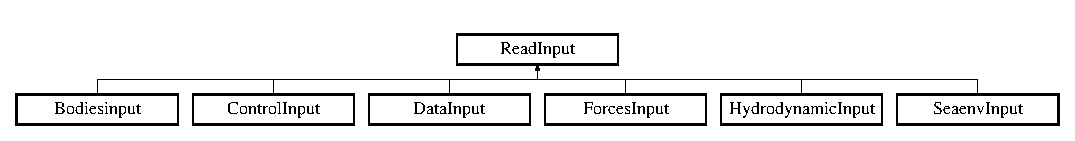
\includegraphics[height=1.447028cm]{class_read_input}
\end{center}
\end{figure}
\subsection*{Public Member Functions}
\begin{DoxyCompactItemize}
\item 
\hyperlink{class_read_input_a181da3d718520ea9168808dde2d3e867}{Read\-Input} ()
\item 
\hyperlink{class_read_input_aec19e94e448ed46207c55412a61728fa}{$\sim$\-Read\-Input} ()
\item 
void \hyperlink{class_read_input_a0cebeb9dda7e4508fdc7a295229b8e07}{set\-Data} (istream \&)
\end{DoxyCompactItemize}
\subsection*{Protected Member Functions}
\begin{DoxyCompactItemize}
\item 
virtual void \hyperlink{class_read_input_a4ff2727b876cfd7c01299b08bdd65646}{initialize\-Defaults} ()=0
\item 
virtual int \hyperlink{class_read_input_a4c67f10e813686bf635dd4c6bb2c61bc}{legal\-Keyword} (string)=0
\item 
virtual bool \hyperlink{class_read_input_a1d8cb0ef59f265300b682de97513f48d}{keyword\-Handler} (int, string, string)=0
\item 
virtual bool \hyperlink{class_read_input_afb66a7ff67d0aeb10a3cfa5a4fbc31f8}{keyword\-Handler} (int, vector$<$ string $>$, bool)=0
\end{DoxyCompactItemize}


\subsection{Detailed Description}
This absract class parses input from file and has functions that must be implemented to handle the data. 

\subsection{Constructor \& Destructor Documentation}
\hypertarget{class_read_input_a181da3d718520ea9168808dde2d3e867}{\index{Read\-Input@{Read\-Input}!Read\-Input@{Read\-Input}}
\index{Read\-Input@{Read\-Input}!ReadInput@{Read\-Input}}
\subsubsection[{Read\-Input}]{\setlength{\rightskip}{0pt plus 5cm}Read\-Input\-::\-Read\-Input (
\begin{DoxyParamCaption}
{}
\end{DoxyParamCaption}
)}}\label{class_read_input_a181da3d718520ea9168808dde2d3e867}
The default constructor. \hypertarget{class_read_input_aec19e94e448ed46207c55412a61728fa}{\index{Read\-Input@{Read\-Input}!$\sim$\-Read\-Input@{$\sim$\-Read\-Input}}
\index{$\sim$\-Read\-Input@{$\sim$\-Read\-Input}!ReadInput@{Read\-Input}}
\subsubsection[{$\sim$\-Read\-Input}]{\setlength{\rightskip}{0pt plus 5cm}Read\-Input\-::$\sim$\-Read\-Input (
\begin{DoxyParamCaption}
{}
\end{DoxyParamCaption}
)}}\label{class_read_input_aec19e94e448ed46207c55412a61728fa}
The default destructor, nothing happens here. 

\subsection{Member Function Documentation}
\hypertarget{class_read_input_a4ff2727b876cfd7c01299b08bdd65646}{\index{Read\-Input@{Read\-Input}!initialize\-Defaults@{initialize\-Defaults}}
\index{initialize\-Defaults@{initialize\-Defaults}!ReadInput@{Read\-Input}}
\subsubsection[{initialize\-Defaults}]{\setlength{\rightskip}{0pt plus 5cm}virtual void Read\-Input\-::initialize\-Defaults (
\begin{DoxyParamCaption}
{}
\end{DoxyParamCaption}
)\hspace{0.3cm}{\ttfamily [protected]}, {\ttfamily [pure virtual]}}}\label{class_read_input_a4ff2727b876cfd7c01299b08bdd65646}
Must be implemented by child class. 

Implemented in \hyperlink{class_control_input_af15fe8b88a0e7f496c7fd0d4795ff900}{Control\-Input}, \hyperlink{class_bodiesinput_ae7c0a7ee2c02e1ed63658a7d06f257e5}{Bodiesinput}, \hyperlink{class_forces_input_a8bcfe50a80d1c2fe11a742081a5e7343}{Forces\-Input}, \hyperlink{class_data_input_a991d4d493aaeaff9d631565b9a49d2ce}{Data\-Input}, \hyperlink{class_seaenv_input_a47a254de1906fcbea59ed961c9a1fc0a}{Seaenv\-Input}, and \hyperlink{class_hydrodynamic_input_a311ec06f62b7929fb6712e90240a1436}{Hydrodynamic\-Input}.

\hypertarget{class_read_input_a1d8cb0ef59f265300b682de97513f48d}{\index{Read\-Input@{Read\-Input}!keyword\-Handler@{keyword\-Handler}}
\index{keyword\-Handler@{keyword\-Handler}!ReadInput@{Read\-Input}}
\subsubsection[{keyword\-Handler}]{\setlength{\rightskip}{0pt plus 5cm}virtual bool Read\-Input\-::keyword\-Handler (
\begin{DoxyParamCaption}
\item[{int}]{, }
\item[{string}]{, }
\item[{string}]{}
\end{DoxyParamCaption}
)\hspace{0.3cm}{\ttfamily [protected]}, {\ttfamily [pure virtual]}}}\label{class_read_input_a1d8cb0ef59f265300b682de97513f48d}
Must be implemented by child class, handles single key/val pairs. 

Implemented in \hyperlink{class_control_input_acb4fb4c1d2a2453e3b8986e44e096f63}{Control\-Input}, \hyperlink{class_bodiesinput_a2bf5785740ebd6e397477e667af16a05}{Bodiesinput}, \hyperlink{class_forces_input_a3e82ee7aa3c5bd35a6bb1b06fcafafa9}{Forces\-Input}, \hyperlink{class_data_input_a80075c8e86436e00c89d891ce0be57a8}{Data\-Input}, and \hyperlink{class_seaenv_input_a79edff5224cca5323f679478c09b1c25}{Seaenv\-Input}.

\hypertarget{class_read_input_afb66a7ff67d0aeb10a3cfa5a4fbc31f8}{\index{Read\-Input@{Read\-Input}!keyword\-Handler@{keyword\-Handler}}
\index{keyword\-Handler@{keyword\-Handler}!ReadInput@{Read\-Input}}
\subsubsection[{keyword\-Handler}]{\setlength{\rightskip}{0pt plus 5cm}virtual bool Read\-Input\-::keyword\-Handler (
\begin{DoxyParamCaption}
\item[{int}]{, }
\item[{vector$<$ string $>$}]{, }
\item[{bool}]{}
\end{DoxyParamCaption}
)\hspace{0.3cm}{\ttfamily [protected]}, {\ttfamily [pure virtual]}}}\label{class_read_input_afb66a7ff67d0aeb10a3cfa5a4fbc31f8}
Must be implemented by child class, handles multiple key/val pairs. 

Implemented in \hyperlink{class_control_input_a33b353c2d8f4316d1543059a319faba7}{Control\-Input}, \hyperlink{class_bodiesinput_af735a952cbd5b1a0c5db67c7209ba847}{Bodiesinput}, \hyperlink{class_forces_input_a52965f2bfde734252e7f4f65bf0fde25}{Forces\-Input}, \hyperlink{class_data_input_a70d0380171a30a659a6c7868f2573c92}{Data\-Input}, and \hyperlink{class_seaenv_input_a3e8d24eadb9f83b1f0ff59cb8de1276e}{Seaenv\-Input}.

\hypertarget{class_read_input_a4c67f10e813686bf635dd4c6bb2c61bc}{\index{Read\-Input@{Read\-Input}!legal\-Keyword@{legal\-Keyword}}
\index{legal\-Keyword@{legal\-Keyword}!ReadInput@{Read\-Input}}
\subsubsection[{legal\-Keyword}]{\setlength{\rightskip}{0pt plus 5cm}virtual int Read\-Input\-::legal\-Keyword (
\begin{DoxyParamCaption}
\item[{string}]{}
\end{DoxyParamCaption}
)\hspace{0.3cm}{\ttfamily [protected]}, {\ttfamily [pure virtual]}}}\label{class_read_input_a4c67f10e813686bf635dd4c6bb2c61bc}
Must be implemented by child class, determine if keyword is legal. 

Implemented in \hyperlink{class_control_input_af7295a9ba455debb812f0e1d4a647820}{Control\-Input}, \hyperlink{class_bodiesinput_abe777be6f9181f1d0f8c5ad523eff6e3}{Bodiesinput}, \hyperlink{class_forces_input_a5f4086acc636b54b64bcd611bdff1aa4}{Forces\-Input}, \hyperlink{class_data_input_ae3ca24179103da6e38b99842b9fc1000}{Data\-Input}, \hyperlink{class_seaenv_input_af0e063c0b66093ed993c79a62c8c092f}{Seaenv\-Input}, and \hyperlink{class_hydrodynamic_input_a6cf4ad1a8407191c8e2633ca0554f641}{Hydrodynamic\-Input}.

\hypertarget{class_read_input_a0cebeb9dda7e4508fdc7a295229b8e07}{\index{Read\-Input@{Read\-Input}!set\-Data@{set\-Data}}
\index{set\-Data@{set\-Data}!ReadInput@{Read\-Input}}
\subsubsection[{set\-Data}]{\setlength{\rightskip}{0pt plus 5cm}void Read\-Input\-::set\-Data (
\begin{DoxyParamCaption}
\item[{istream \&}]{infile}
\end{DoxyParamCaption}
)}}\label{class_read_input_a0cebeb9dda7e4508fdc7a295229b8e07}
Parses input files and handles the data. 
\begin{DoxyParams}{Parameters}
{\em infile} & The file that is currently being read in by the parser. \\
\hline
\end{DoxyParams}


The documentation for this class was generated from the following files\-:\begin{DoxyCompactItemize}
\item 
Visual Studio 2010/\-Projects/o\-Freq Windows V\-S2010/o\-Freq/readinputfile.\-h\item 
Visual Studio 2010/\-Projects/o\-Freq Windows V\-S2010/o\-Freq/readinputfile.\-cpp\end{DoxyCompactItemize}

\hypertarget{class_seaenv_input}{\section{Seaenv\-Input Class Reference}
\label{class_seaenv_input}\index{Seaenv\-Input@{Seaenv\-Input}}
}


{\ttfamily \#include $<$seaenvinput.\-h$>$}

Inheritance diagram for Seaenv\-Input\-:\begin{figure}[H]
\begin{center}
\leavevmode
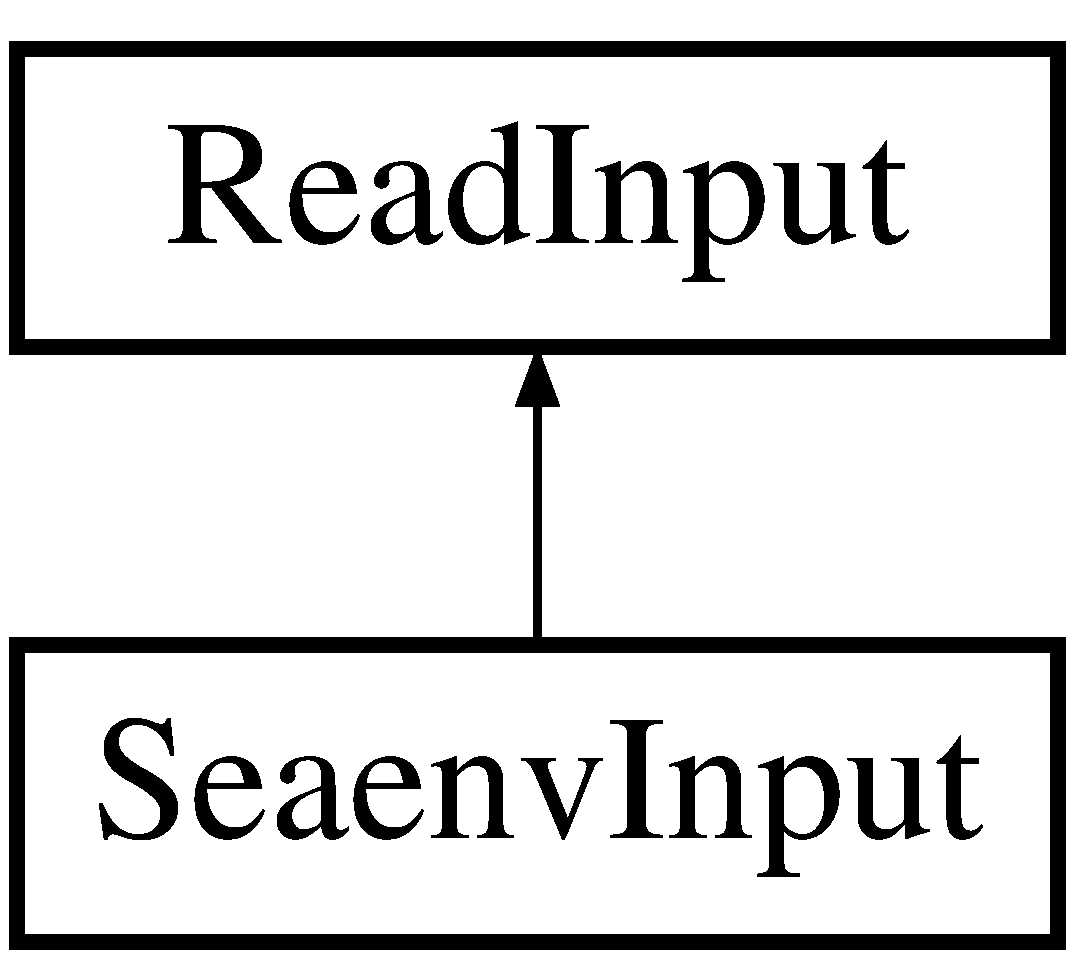
\includegraphics[height=2.000000cm]{class_seaenv_input}
\end{center}
\end{figure}
\subsection*{Public Member Functions}
\begin{DoxyCompactItemize}
\item 
\hyperlink{class_seaenv_input_a1d4cf4bbf2effd0d558b7b97b02a092a}{Seaenv\-Input} ()
\item 
\hyperlink{class_seaenv_input_a1211270b8f35af72156e623852ce85a7}{$\sim$\-Seaenv\-Input} ()
\item 
void \hyperlink{class_seaenv_input_af215cdefc653fb335dc68de34962201f}{test\-Print} ()
\end{DoxyCompactItemize}
\subsection*{Protected Member Functions}
\begin{DoxyCompactItemize}
\item 
void \hyperlink{class_seaenv_input_a47a254de1906fcbea59ed961c9a1fc0a}{initialize\-Defaults} ()
\item 
int \hyperlink{class_seaenv_input_af0e063c0b66093ed993c79a62c8c092f}{legal\-Keyword} (string)
\item 
bool \hyperlink{class_seaenv_input_a79edff5224cca5323f679478c09b1c25}{keyword\-Handler} (int, string, string)
\item 
bool \hyperlink{class_seaenv_input_a3e8d24eadb9f83b1f0ff59cb8de1276e}{keyword\-Handler} (int, vector$<$ string $>$, bool)
\end{DoxyCompactItemize}


\subsection{Detailed Description}
This class parses input from file and stores the data appropriately in the \hyperlink{class_sea_enviroment}{Sea\-Enviroment} object. 

\subsection{Constructor \& Destructor Documentation}
\hypertarget{class_seaenv_input_a1d4cf4bbf2effd0d558b7b97b02a092a}{\index{Seaenv\-Input@{Seaenv\-Input}!Seaenv\-Input@{Seaenv\-Input}}
\index{Seaenv\-Input@{Seaenv\-Input}!SeaenvInput@{Seaenv\-Input}}
\subsubsection[{Seaenv\-Input}]{\setlength{\rightskip}{0pt plus 5cm}Seaenv\-Input\-::\-Seaenv\-Input (
\begin{DoxyParamCaption}
{}
\end{DoxyParamCaption}
)}}\label{class_seaenv_input_a1d4cf4bbf2effd0d558b7b97b02a092a}
The default constructor. \hypertarget{class_seaenv_input_a1211270b8f35af72156e623852ce85a7}{\index{Seaenv\-Input@{Seaenv\-Input}!$\sim$\-Seaenv\-Input@{$\sim$\-Seaenv\-Input}}
\index{$\sim$\-Seaenv\-Input@{$\sim$\-Seaenv\-Input}!SeaenvInput@{Seaenv\-Input}}
\subsubsection[{$\sim$\-Seaenv\-Input}]{\setlength{\rightskip}{0pt plus 5cm}Seaenv\-Input\-::$\sim$\-Seaenv\-Input (
\begin{DoxyParamCaption}
{}
\end{DoxyParamCaption}
)}}\label{class_seaenv_input_a1211270b8f35af72156e623852ce85a7}
The default destructor, nothing happens here. 

\subsection{Member Function Documentation}
\hypertarget{class_seaenv_input_a47a254de1906fcbea59ed961c9a1fc0a}{\index{Seaenv\-Input@{Seaenv\-Input}!initialize\-Defaults@{initialize\-Defaults}}
\index{initialize\-Defaults@{initialize\-Defaults}!SeaenvInput@{Seaenv\-Input}}
\subsubsection[{initialize\-Defaults}]{\setlength{\rightskip}{0pt plus 5cm}void Seaenv\-Input\-::initialize\-Defaults (
\begin{DoxyParamCaption}
{}
\end{DoxyParamCaption}
)\hspace{0.3cm}{\ttfamily [protected]}, {\ttfamily [virtual]}}}\label{class_seaenv_input_a47a254de1906fcbea59ed961c9a1fc0a}
For future use, does nothing as of now. 

Implements \hyperlink{class_read_input_a4ff2727b876cfd7c01299b08bdd65646}{Read\-Input}.

\hypertarget{class_seaenv_input_a79edff5224cca5323f679478c09b1c25}{\index{Seaenv\-Input@{Seaenv\-Input}!keyword\-Handler@{keyword\-Handler}}
\index{keyword\-Handler@{keyword\-Handler}!SeaenvInput@{Seaenv\-Input}}
\subsubsection[{keyword\-Handler}]{\setlength{\rightskip}{0pt plus 5cm}bool Seaenv\-Input\-::keyword\-Handler (
\begin{DoxyParamCaption}
\item[{int}]{key\-Control, }
\item[{string}]{identifier, }
\item[{string}]{val}
\end{DoxyParamCaption}
)\hspace{0.3cm}{\ttfamily [protected]}, {\ttfamily [virtual]}}}\label{class_seaenv_input_a79edff5224cca5323f679478c09b1c25}
Stores the data if valid keyword according to the legeal\-Keyword function. 
\begin{DoxyParams}{Parameters}
{\em key\-Control} & Indicated which case in switch function to use. \\
\hline
{\em identifier} & The keyword. \\
\hline
{\em val} & The value associated with the keyword. \\
\hline
\end{DoxyParams}
\begin{DoxyReturn}{Returns}
false if not done reading data, true to move onto next keyword in parser. 
\end{DoxyReturn}


Implements \hyperlink{class_read_input_a1d8cb0ef59f265300b682de97513f48d}{Read\-Input}.

\hypertarget{class_seaenv_input_a3e8d24eadb9f83b1f0ff59cb8de1276e}{\index{Seaenv\-Input@{Seaenv\-Input}!keyword\-Handler@{keyword\-Handler}}
\index{keyword\-Handler@{keyword\-Handler}!SeaenvInput@{Seaenv\-Input}}
\subsubsection[{keyword\-Handler}]{\setlength{\rightskip}{0pt plus 5cm}bool Seaenv\-Input\-::keyword\-Handler (
\begin{DoxyParamCaption}
\item[{int}]{key\-Control, }
\item[{vector$<$ string $>$}]{the\-List\-In, }
\item[{bool}]{is\-Direct}
\end{DoxyParamCaption}
)\hspace{0.3cm}{\ttfamily [protected]}, {\ttfamily [virtual]}}}\label{class_seaenv_input_a3e8d24eadb9f83b1f0ff59cb8de1276e}
Stores the list data if valid keyword according to the legeal\-Keyword function. 
\begin{DoxyParams}{Parameters}
{\em key\-Control} & Indicated which case in switch function to use. \\
\hline
{\em the\-List\-In} & List of Values. \\
\hline
{\em is\-Direct} & True if Direct Access List, False if Sequenctial List. \\
\hline
\end{DoxyParams}
\begin{DoxyReturn}{Returns}
false if not done reading data, true to move onto next keyword in parser. 
\end{DoxyReturn}


Implements \hyperlink{class_read_input_afb66a7ff67d0aeb10a3cfa5a4fbc31f8}{Read\-Input}.

\hypertarget{class_seaenv_input_af0e063c0b66093ed993c79a62c8c092f}{\index{Seaenv\-Input@{Seaenv\-Input}!legal\-Keyword@{legal\-Keyword}}
\index{legal\-Keyword@{legal\-Keyword}!SeaenvInput@{Seaenv\-Input}}
\subsubsection[{legal\-Keyword}]{\setlength{\rightskip}{0pt plus 5cm}int Seaenv\-Input\-::legal\-Keyword (
\begin{DoxyParamCaption}
\item[{string}]{string\-In}
\end{DoxyParamCaption}
)\hspace{0.3cm}{\ttfamily [protected]}, {\ttfamily [virtual]}}}\label{class_seaenv_input_af0e063c0b66093ed993c79a62c8c092f}
Returns int greater than 0 if the keyword is legal, the int returned specifies how to handle data in keyword\-Handler. 
\begin{DoxyParams}{Parameters}
{\em string\-In} & Check if a valid keyword. \\
\hline
\end{DoxyParams}
\begin{DoxyReturn}{Returns}
int value which tells keyword\-Handler how to handle the data. 
\end{DoxyReturn}


Implements \hyperlink{class_read_input_a4c67f10e813686bf635dd4c6bb2c61bc}{Read\-Input}.

\hypertarget{class_seaenv_input_af215cdefc653fb335dc68de34962201f}{\index{Seaenv\-Input@{Seaenv\-Input}!test\-Print@{test\-Print}}
\index{test\-Print@{test\-Print}!SeaenvInput@{Seaenv\-Input}}
\subsubsection[{test\-Print}]{\setlength{\rightskip}{0pt plus 5cm}void Seaenv\-Input\-::test\-Print (
\begin{DoxyParamCaption}
{}
\end{DoxyParamCaption}
)}}\label{class_seaenv_input_af215cdefc653fb335dc68de34962201f}
Print to console all data members. 

The documentation for this class was generated from the following files\-:\begin{DoxyCompactItemize}
\item 
Visual Studio 2010/\-Projects/o\-Freq Windows V\-S2010/o\-Freq/seaenvinput.\-h\item 
Visual Studio 2010/\-Projects/o\-Freq Windows V\-S2010/o\-Freq/seaenvinput.\-cpp\end{DoxyCompactItemize}

\hypertarget{class_sea_enviroment}{\section{Sea\-Enviroment Class Reference}
\label{class_sea_enviroment}\index{Sea\-Enviroment@{Sea\-Enviroment}}
}


{\ttfamily \#include $<$seaenviroment.\-h$>$}

\subsection*{Public Member Functions}
\begin{DoxyCompactItemize}
\item 
\hyperlink{class_sea_enviroment_af76135d3915bfc5e5ff526d5f61379b5}{Sea\-Enviroment} ()
\item 
\hyperlink{class_sea_enviroment_ae287606b637f6bf2bae1ab15b4bd6ead}{$\sim$\-Sea\-Enviroment} ()
\item 
void \hyperlink{class_sea_enviroment_a565628f92f230b23a144efba806db5d5}{test\-Print} ()
\item 
void \hyperlink{class_sea_enviroment_a8ec14b498399f23522f0b934b0dfee6d}{set\-Wave\-Spectrum\-Name} (string)
\item 
void \hyperlink{class_sea_enviroment_a61e0801c1942de481e1b9a0c38484792}{set\-Wave\-Spectrum\-Frequencies} (vector$<$ double $>$)
\item 
void \hyperlink{class_sea_enviroment_a6a0904d98840e33e78f67ac4a2d66636}{set\-Wave\-Spectrum\-Wave\-Energy} (vector$<$ double $>$)
\item 
void \hyperlink{class_sea_enviroment_a9ccfefa30c3f71dc0f72687435aa8e58}{set\-Spread\-Model\-Name} (string)
\item 
void \hyperlink{class_sea_enviroment_a85a797df8c4fe557b6ec9173434a0032}{set\-Spread\-Model\-Direction\-Angle} (double)
\item 
void \hyperlink{class_sea_enviroment_a7abfe63a9de261aa79ed90cf83347999}{set\-Spread\-Model\-Wave\-Spectrum\-Name} (string)
\item 
void \hyperlink{class_sea_enviroment_a8f2f360969e05ebcb478258ec4fd6077}{set\-Spread\-Model\-Scaling\-Factor} (double)
\end{DoxyCompactItemize}


\subsection{Detailed Description}
This class holds all data for the sea enviroment. 

\subsection{Constructor \& Destructor Documentation}
\hypertarget{class_sea_enviroment_af76135d3915bfc5e5ff526d5f61379b5}{\index{Sea\-Enviroment@{Sea\-Enviroment}!Sea\-Enviroment@{Sea\-Enviroment}}
\index{Sea\-Enviroment@{Sea\-Enviroment}!SeaEnviroment@{Sea\-Enviroment}}
\subsubsection[{Sea\-Enviroment}]{\setlength{\rightskip}{0pt plus 5cm}Sea\-Enviroment\-::\-Sea\-Enviroment (
\begin{DoxyParamCaption}
{}
\end{DoxyParamCaption}
)}}\label{class_sea_enviroment_af76135d3915bfc5e5ff526d5f61379b5}
The default constructor. \hypertarget{class_sea_enviroment_ae287606b637f6bf2bae1ab15b4bd6ead}{\index{Sea\-Enviroment@{Sea\-Enviroment}!$\sim$\-Sea\-Enviroment@{$\sim$\-Sea\-Enviroment}}
\index{$\sim$\-Sea\-Enviroment@{$\sim$\-Sea\-Enviroment}!SeaEnviroment@{Sea\-Enviroment}}
\subsubsection[{$\sim$\-Sea\-Enviroment}]{\setlength{\rightskip}{0pt plus 5cm}Sea\-Enviroment\-::$\sim$\-Sea\-Enviroment (
\begin{DoxyParamCaption}
{}
\end{DoxyParamCaption}
)}}\label{class_sea_enviroment_ae287606b637f6bf2bae1ab15b4bd6ead}
The default destructor, nothing happens here. 

\subsection{Member Function Documentation}
\hypertarget{class_sea_enviroment_a85a797df8c4fe557b6ec9173434a0032}{\index{Sea\-Enviroment@{Sea\-Enviroment}!set\-Spread\-Model\-Direction\-Angle@{set\-Spread\-Model\-Direction\-Angle}}
\index{set\-Spread\-Model\-Direction\-Angle@{set\-Spread\-Model\-Direction\-Angle}!SeaEnviroment@{Sea\-Enviroment}}
\subsubsection[{set\-Spread\-Model\-Direction\-Angle}]{\setlength{\rightskip}{0pt plus 5cm}void Sea\-Enviroment\-::set\-Spread\-Model\-Direction\-Angle (
\begin{DoxyParamCaption}
\item[{double}]{val}
\end{DoxyParamCaption}
)}}\label{class_sea_enviroment_a85a797df8c4fe557b6ec9173434a0032}
Sets spread model direction angle. 
\begin{DoxyParams}{Parameters}
{\em val} & The direction angle. \\
\hline
\end{DoxyParams}
\hypertarget{class_sea_enviroment_a9ccfefa30c3f71dc0f72687435aa8e58}{\index{Sea\-Enviroment@{Sea\-Enviroment}!set\-Spread\-Model\-Name@{set\-Spread\-Model\-Name}}
\index{set\-Spread\-Model\-Name@{set\-Spread\-Model\-Name}!SeaEnviroment@{Sea\-Enviroment}}
\subsubsection[{set\-Spread\-Model\-Name}]{\setlength{\rightskip}{0pt plus 5cm}void Sea\-Enviroment\-::set\-Spread\-Model\-Name (
\begin{DoxyParamCaption}
\item[{string}]{new\-Name}
\end{DoxyParamCaption}
)}}\label{class_sea_enviroment_a9ccfefa30c3f71dc0f72687435aa8e58}
Sets the spread model name. 
\begin{DoxyParams}{Parameters}
{\em new\-Name} & The name of the spread model to be used. \\
\hline
\end{DoxyParams}
\hypertarget{class_sea_enviroment_a8f2f360969e05ebcb478258ec4fd6077}{\index{Sea\-Enviroment@{Sea\-Enviroment}!set\-Spread\-Model\-Scaling\-Factor@{set\-Spread\-Model\-Scaling\-Factor}}
\index{set\-Spread\-Model\-Scaling\-Factor@{set\-Spread\-Model\-Scaling\-Factor}!SeaEnviroment@{Sea\-Enviroment}}
\subsubsection[{set\-Spread\-Model\-Scaling\-Factor}]{\setlength{\rightskip}{0pt plus 5cm}void Sea\-Enviroment\-::set\-Spread\-Model\-Scaling\-Factor (
\begin{DoxyParamCaption}
\item[{double}]{val}
\end{DoxyParamCaption}
)}}\label{class_sea_enviroment_a8f2f360969e05ebcb478258ec4fd6077}
Sets scaling factor. 
\begin{DoxyParams}{Parameters}
{\em val} & The scaling factor. \\
\hline
\end{DoxyParams}
\hypertarget{class_sea_enviroment_a7abfe63a9de261aa79ed90cf83347999}{\index{Sea\-Enviroment@{Sea\-Enviroment}!set\-Spread\-Model\-Wave\-Spectrum\-Name@{set\-Spread\-Model\-Wave\-Spectrum\-Name}}
\index{set\-Spread\-Model\-Wave\-Spectrum\-Name@{set\-Spread\-Model\-Wave\-Spectrum\-Name}!SeaEnviroment@{Sea\-Enviroment}}
\subsubsection[{set\-Spread\-Model\-Wave\-Spectrum\-Name}]{\setlength{\rightskip}{0pt plus 5cm}void Sea\-Enviroment\-::set\-Spread\-Model\-Wave\-Spectrum\-Name (
\begin{DoxyParamCaption}
\item[{string}]{new\-Name}
\end{DoxyParamCaption}
)}}\label{class_sea_enviroment_a7abfe63a9de261aa79ed90cf83347999}
Sets spread model direction angle. 
\begin{DoxyParams}{Parameters}
{\em new\-Name} & The name of the wave spectrum. \\
\hline
\end{DoxyParams}
\hypertarget{class_sea_enviroment_a61e0801c1942de481e1b9a0c38484792}{\index{Sea\-Enviroment@{Sea\-Enviroment}!set\-Wave\-Spectrum\-Frequencies@{set\-Wave\-Spectrum\-Frequencies}}
\index{set\-Wave\-Spectrum\-Frequencies@{set\-Wave\-Spectrum\-Frequencies}!SeaEnviroment@{Sea\-Enviroment}}
\subsubsection[{set\-Wave\-Spectrum\-Frequencies}]{\setlength{\rightskip}{0pt plus 5cm}void Sea\-Enviroment\-::set\-Wave\-Spectrum\-Frequencies (
\begin{DoxyParamCaption}
\item[{vector$<$ double $>$}]{vec\-In}
\end{DoxyParamCaption}
)}}\label{class_sea_enviroment_a61e0801c1942de481e1b9a0c38484792}
Sets the wave frequencies. 
\begin{DoxyParams}{Parameters}
{\em vec\-In} & The list of wave frequencies. \\
\hline
\end{DoxyParams}
\hypertarget{class_sea_enviroment_a8ec14b498399f23522f0b934b0dfee6d}{\index{Sea\-Enviroment@{Sea\-Enviroment}!set\-Wave\-Spectrum\-Name@{set\-Wave\-Spectrum\-Name}}
\index{set\-Wave\-Spectrum\-Name@{set\-Wave\-Spectrum\-Name}!SeaEnviroment@{Sea\-Enviroment}}
\subsubsection[{set\-Wave\-Spectrum\-Name}]{\setlength{\rightskip}{0pt plus 5cm}void Sea\-Enviroment\-::set\-Wave\-Spectrum\-Name (
\begin{DoxyParamCaption}
\item[{string}]{new\-Name}
\end{DoxyParamCaption}
)}}\label{class_sea_enviroment_a8ec14b498399f23522f0b934b0dfee6d}
Sets the wave spectrum. 
\begin{DoxyParams}{Parameters}
{\em new\-Name} & The name of the wave spectrum. \\
\hline
\end{DoxyParams}
\hypertarget{class_sea_enviroment_a6a0904d98840e33e78f67ac4a2d66636}{\index{Sea\-Enviroment@{Sea\-Enviroment}!set\-Wave\-Spectrum\-Wave\-Energy@{set\-Wave\-Spectrum\-Wave\-Energy}}
\index{set\-Wave\-Spectrum\-Wave\-Energy@{set\-Wave\-Spectrum\-Wave\-Energy}!SeaEnviroment@{Sea\-Enviroment}}
\subsubsection[{set\-Wave\-Spectrum\-Wave\-Energy}]{\setlength{\rightskip}{0pt plus 5cm}void Sea\-Enviroment\-::set\-Wave\-Spectrum\-Wave\-Energy (
\begin{DoxyParamCaption}
\item[{vector$<$ double $>$}]{vec\-In}
\end{DoxyParamCaption}
)}}\label{class_sea_enviroment_a6a0904d98840e33e78f67ac4a2d66636}
Sets the wave energy. 
\begin{DoxyParams}{Parameters}
{\em vec\-In} & The list of wave energy. \\
\hline
\end{DoxyParams}
\hypertarget{class_sea_enviroment_a565628f92f230b23a144efba806db5d5}{\index{Sea\-Enviroment@{Sea\-Enviroment}!test\-Print@{test\-Print}}
\index{test\-Print@{test\-Print}!SeaEnviroment@{Sea\-Enviroment}}
\subsubsection[{test\-Print}]{\setlength{\rightskip}{0pt plus 5cm}void Sea\-Enviroment\-::test\-Print (
\begin{DoxyParamCaption}
{}
\end{DoxyParamCaption}
)}}\label{class_sea_enviroment_a565628f92f230b23a144efba806db5d5}
Test print to console the values of all data members. 

The documentation for this class was generated from the following files\-:\begin{DoxyCompactItemize}
\item 
Visual Studio 2010/\-Projects/o\-Freq Windows V\-S2010/o\-Freq/seaenviroment.\-h\item 
Visual Studio 2010/\-Projects/o\-Freq Windows V\-S2010/o\-Freq/seaenviroment.\-cpp\end{DoxyCompactItemize}

\hypertarget{class_system}{\section{System Class Reference}
\label{class_system}\index{System@{System}}
}


{\ttfamily \#include $<$system.\-h$>$}

\subsection*{Public Member Functions}
\begin{DoxyCompactItemize}
\item 
\hyperlink{class_system_ae317936c9bcf1374d61745572e0f2f8a}{System} ()
\item 
\hyperlink{class_system_a3be70bb338e3f062f821173fd15680d0}{$\sim$\-System} ()
\item 
void \hyperlink{class_system_a20bda2428f8aef211bf8787e1efeeeee}{test\-Print} ()
\item 
void \hyperlink{class_system_ae58c969c9ba0a1ec4bebff64b88a22ed}{set\-Analysis\-Type} (string)
\item 
void \hyperlink{class_system_ab1bfe916791d4c61bb807c930f73930c}{set\-Wave\-Frequencies} (vector$<$ double $>$)
\item 
void \hyperlink{class_system_a492b1dc5f789192ff6207f2555b23138}{set\-Wave\-Directions} (vector$<$ double $>$)
\item 
void \hyperlink{class_system_a2c26340bdbd94e6bed0f75dba991b49c}{set\-Spread\-Model} (string)
\item 
vector$<$ double $>$ \hyperlink{class_system_a18b18022b6468a41dfdbfc49c881b933}{get\-Wave\-Frequencies} ()
\item 
vector$<$ double $>$ \hyperlink{class_system_a8e1d633a4b604223236e4cc4de35bd70}{get\-Wave\-Directions} ()
\end{DoxyCompactItemize}


\subsection{Detailed Description}
This class holds data for the system object. 

\subsection{Constructor \& Destructor Documentation}
\hypertarget{class_system_ae317936c9bcf1374d61745572e0f2f8a}{\index{System@{System}!System@{System}}
\index{System@{System}!System@{System}}
\subsubsection[{System}]{\setlength{\rightskip}{0pt plus 5cm}System\-::\-System (
\begin{DoxyParamCaption}
{}
\end{DoxyParamCaption}
)}}\label{class_system_ae317936c9bcf1374d61745572e0f2f8a}
The default constructor. \hypertarget{class_system_a3be70bb338e3f062f821173fd15680d0}{\index{System@{System}!$\sim$\-System@{$\sim$\-System}}
\index{$\sim$\-System@{$\sim$\-System}!System@{System}}
\subsubsection[{$\sim$\-System}]{\setlength{\rightskip}{0pt plus 5cm}System\-::$\sim$\-System (
\begin{DoxyParamCaption}
{}
\end{DoxyParamCaption}
)}}\label{class_system_a3be70bb338e3f062f821173fd15680d0}
The default destructor, nothing happens here. 

\subsection{Member Function Documentation}
\hypertarget{class_system_a8e1d633a4b604223236e4cc4de35bd70}{\index{System@{System}!get\-Wave\-Directions@{get\-Wave\-Directions}}
\index{get\-Wave\-Directions@{get\-Wave\-Directions}!System@{System}}
\subsubsection[{get\-Wave\-Directions}]{\setlength{\rightskip}{0pt plus 5cm}vector$<$ double $>$ System\-::get\-Wave\-Directions (
\begin{DoxyParamCaption}
{}
\end{DoxyParamCaption}
)}}\label{class_system_a8e1d633a4b604223236e4cc4de35bd70}
Retrieve the list of wave directions. \begin{DoxyReturn}{Returns}
The list of wave directions. 
\end{DoxyReturn}
\hypertarget{class_system_a18b18022b6468a41dfdbfc49c881b933}{\index{System@{System}!get\-Wave\-Frequencies@{get\-Wave\-Frequencies}}
\index{get\-Wave\-Frequencies@{get\-Wave\-Frequencies}!System@{System}}
\subsubsection[{get\-Wave\-Frequencies}]{\setlength{\rightskip}{0pt plus 5cm}vector$<$ double $>$ System\-::get\-Wave\-Frequencies (
\begin{DoxyParamCaption}
{}
\end{DoxyParamCaption}
)}}\label{class_system_a18b18022b6468a41dfdbfc49c881b933}
Retrieve the list of wave frequencies. \begin{DoxyReturn}{Returns}
The list of wave frequencies. 
\end{DoxyReturn}
\hypertarget{class_system_ae58c969c9ba0a1ec4bebff64b88a22ed}{\index{System@{System}!set\-Analysis\-Type@{set\-Analysis\-Type}}
\index{set\-Analysis\-Type@{set\-Analysis\-Type}!System@{System}}
\subsubsection[{set\-Analysis\-Type}]{\setlength{\rightskip}{0pt plus 5cm}void System\-::set\-Analysis\-Type (
\begin{DoxyParamCaption}
\item[{string}]{analysis\-Type\-In}
\end{DoxyParamCaption}
)}}\label{class_system_ae58c969c9ba0a1ec4bebff64b88a22ed}
Sets the analysis ype. 
\begin{DoxyParams}{Parameters}
{\em analysis\-Type\-In} & The analysis type. \\
\hline
\end{DoxyParams}
\hypertarget{class_system_a2c26340bdbd94e6bed0f75dba991b49c}{\index{System@{System}!set\-Spread\-Model@{set\-Spread\-Model}}
\index{set\-Spread\-Model@{set\-Spread\-Model}!System@{System}}
\subsubsection[{set\-Spread\-Model}]{\setlength{\rightskip}{0pt plus 5cm}void System\-::set\-Spread\-Model (
\begin{DoxyParamCaption}
\item[{string}]{spread\-In}
\end{DoxyParamCaption}
)}}\label{class_system_a2c26340bdbd94e6bed0f75dba991b49c}
Sets the spread model. 
\begin{DoxyParams}{Parameters}
{\em spread\-In} & The spread model. \\
\hline
\end{DoxyParams}
\hypertarget{class_system_a492b1dc5f789192ff6207f2555b23138}{\index{System@{System}!set\-Wave\-Directions@{set\-Wave\-Directions}}
\index{set\-Wave\-Directions@{set\-Wave\-Directions}!System@{System}}
\subsubsection[{set\-Wave\-Directions}]{\setlength{\rightskip}{0pt plus 5cm}void System\-::set\-Wave\-Directions (
\begin{DoxyParamCaption}
\item[{vector$<$ double $>$}]{vec\-In}
\end{DoxyParamCaption}
)}}\label{class_system_a492b1dc5f789192ff6207f2555b23138}
Sets the wave directions. 
\begin{DoxyParams}{Parameters}
{\em vec\-In} & The list of wave directions. \\
\hline
\end{DoxyParams}
\hypertarget{class_system_ab1bfe916791d4c61bb807c930f73930c}{\index{System@{System}!set\-Wave\-Frequencies@{set\-Wave\-Frequencies}}
\index{set\-Wave\-Frequencies@{set\-Wave\-Frequencies}!System@{System}}
\subsubsection[{set\-Wave\-Frequencies}]{\setlength{\rightskip}{0pt plus 5cm}void System\-::set\-Wave\-Frequencies (
\begin{DoxyParamCaption}
\item[{vector$<$ double $>$}]{vec\-In}
\end{DoxyParamCaption}
)}}\label{class_system_ab1bfe916791d4c61bb807c930f73930c}
Sets the wave frequencies. 
\begin{DoxyParams}{Parameters}
{\em vec\-In} & The list of wave frequencies. \\
\hline
\end{DoxyParams}
\hypertarget{class_system_a20bda2428f8aef211bf8787e1efeeeee}{\index{System@{System}!test\-Print@{test\-Print}}
\index{test\-Print@{test\-Print}!System@{System}}
\subsubsection[{test\-Print}]{\setlength{\rightskip}{0pt plus 5cm}void System\-::test\-Print (
\begin{DoxyParamCaption}
{}
\end{DoxyParamCaption}
)}}\label{class_system_a20bda2428f8aef211bf8787e1efeeeee}
Test print to console the values of all data members. 

The documentation for this class was generated from the following files\-:\begin{DoxyCompactItemize}
\item 
Visual Studio 2010/\-Projects/o\-Freq Windows V\-S2010/o\-Freq/system.\-h\item 
Visual Studio 2010/\-Projects/o\-Freq Windows V\-S2010/o\-Freq/system.\-cpp\end{DoxyCompactItemize}

\hypertarget{class_user_forces}{\section{User\-Forces Class Reference}
\label{class_user_forces}\index{User\-Forces@{User\-Forces}}
}


{\ttfamily \#include $<$userforces.\-h$>$}

\subsection*{Public Member Functions}
\begin{DoxyCompactItemize}
\item 
\hyperlink{class_user_forces_a642cb07c929ac7431ba9b9bd1cf62487}{User\-Forces} ()
\item 
\hyperlink{class_user_forces_aae54a625e8d3a753b108c47e543a9b3c}{$\sim$\-User\-Forces} ()
\item 
void \hyperlink{class_user_forces_af4543aab611d78a96c2c3ccd8a182c43}{add\-New\-Force} (string)
\item 
void \hyperlink{class_user_forces_a5e91ea4efcb7bfea69fac4707b0f7523}{set\-Coeff} (vector$<$ string $>$, bool)
\item 
void \hyperlink{class_user_forces_ac9af0ed1756485df7f1c20434a419430}{set\-Order\-Derivative} (int)
\item 
void \hyperlink{class_user_forces_a701bdb1ef5b9b9d323a3064d57009073}{set\-Equation\-Number} (int)
\item 
void \hyperlink{class_user_forces_acf637eb58f211a30292a56579523c8b6}{set\-Cur\-Force\-As\-Active} ()
\item 
void \hyperlink{class_user_forces_a9ef4176430e8ac2f087277f4fe359a85}{set\-Cur\-Force\-As\-Reactive} ()
\item 
void \hyperlink{class_user_forces_aeee89b5918595cdc8e573e634bc48e29}{set\-Cur\-Force\-As\-Cross\-Body} ()
\item 
void \hyperlink{class_user_forces_ab5af72b01b05992885c2f32f924103dc}{test\-Print} ()
\item 
vector$<$ complex\-Double $>$ \hyperlink{class_user_forces_a972c3378118f3ebce036a5be3914657b}{get\-User\-Active\-Force} (string)
\item 
vector$<$ \hyperlink{class_derivative}{Derivative} $>$ \hyperlink{class_user_forces_adb47c57e211381745905ad88831a30ac}{get\-User\-Reactive\-Force} (string)
\item 
vector$<$ \hyperlink{class_derivative}{Derivative} $>$ \hyperlink{class_user_forces_a234c94ba061fcfff579fb1dd8bc1a47d}{get\-User\-Cross\-Body\-Force} (string)
\end{DoxyCompactItemize}


\subsection{Detailed Description}
This class holds all of the data for the forces objects. 

\subsection{Constructor \& Destructor Documentation}
\hypertarget{class_user_forces_a642cb07c929ac7431ba9b9bd1cf62487}{\index{User\-Forces@{User\-Forces}!User\-Forces@{User\-Forces}}
\index{User\-Forces@{User\-Forces}!UserForces@{User\-Forces}}
\subsubsection[{User\-Forces}]{\setlength{\rightskip}{0pt plus 5cm}User\-Forces\-::\-User\-Forces (
\begin{DoxyParamCaption}
{}
\end{DoxyParamCaption}
)}}\label{class_user_forces_a642cb07c929ac7431ba9b9bd1cf62487}
The default constructor \hypertarget{class_user_forces_aae54a625e8d3a753b108c47e543a9b3c}{\index{User\-Forces@{User\-Forces}!$\sim$\-User\-Forces@{$\sim$\-User\-Forces}}
\index{$\sim$\-User\-Forces@{$\sim$\-User\-Forces}!UserForces@{User\-Forces}}
\subsubsection[{$\sim$\-User\-Forces}]{\setlength{\rightskip}{0pt plus 5cm}User\-Forces\-::$\sim$\-User\-Forces (
\begin{DoxyParamCaption}
{}
\end{DoxyParamCaption}
)}}\label{class_user_forces_aae54a625e8d3a753b108c47e543a9b3c}
The default destructor, nothing happens here. 

\subsection{Member Function Documentation}
\hypertarget{class_user_forces_af4543aab611d78a96c2c3ccd8a182c43}{\index{User\-Forces@{User\-Forces}!add\-New\-Force@{add\-New\-Force}}
\index{add\-New\-Force@{add\-New\-Force}!UserForces@{User\-Forces}}
\subsubsection[{add\-New\-Force}]{\setlength{\rightskip}{0pt plus 5cm}void User\-Forces\-::add\-New\-Force (
\begin{DoxyParamCaption}
\item[{string}]{new\-Force\-Name}
\end{DoxyParamCaption}
)}}\label{class_user_forces_af4543aab611d78a96c2c3ccd8a182c43}
Adds a new force to the list. 
\begin{DoxyParams}{Parameters}
{\em new\-Force\-Name} & The name of the force. \\
\hline
\end{DoxyParams}
\hypertarget{class_user_forces_a972c3378118f3ebce036a5be3914657b}{\index{User\-Forces@{User\-Forces}!get\-User\-Active\-Force@{get\-User\-Active\-Force}}
\index{get\-User\-Active\-Force@{get\-User\-Active\-Force}!UserForces@{User\-Forces}}
\subsubsection[{get\-User\-Active\-Force}]{\setlength{\rightskip}{0pt plus 5cm}vector$<$ complex\-Double $>$ User\-Forces\-::get\-User\-Active\-Force (
\begin{DoxyParamCaption}
\item[{string}]{active\-Force\-Name}
\end{DoxyParamCaption}
)}}\label{class_user_forces_a972c3378118f3ebce036a5be3914657b}
Retrieve the active force by name. 
\begin{DoxyParams}{Parameters}
{\em active\-Force\-Name} & The name of the active force. \\
\hline
\end{DoxyParams}
\begin{DoxyReturn}{Returns}
Return the active force if found. 
\end{DoxyReturn}
\hypertarget{class_user_forces_a234c94ba061fcfff579fb1dd8bc1a47d}{\index{User\-Forces@{User\-Forces}!get\-User\-Cross\-Body\-Force@{get\-User\-Cross\-Body\-Force}}
\index{get\-User\-Cross\-Body\-Force@{get\-User\-Cross\-Body\-Force}!UserForces@{User\-Forces}}
\subsubsection[{get\-User\-Cross\-Body\-Force}]{\setlength{\rightskip}{0pt plus 5cm}vector$<$ {\bf Derivative} $>$ User\-Forces\-::get\-User\-Cross\-Body\-Force (
\begin{DoxyParamCaption}
\item[{string}]{cross\-Body\-Force\-Name}
\end{DoxyParamCaption}
)}}\label{class_user_forces_a234c94ba061fcfff579fb1dd8bc1a47d}
Retrieve the cross body force by name. 
\begin{DoxyParams}{Parameters}
{\em cross\-Body\-Force\-Name} & The name of the cross body force. \\
\hline
\end{DoxyParams}
\begin{DoxyReturn}{Returns}
Return the cross body force if found. 
\end{DoxyReturn}
\hypertarget{class_user_forces_adb47c57e211381745905ad88831a30ac}{\index{User\-Forces@{User\-Forces}!get\-User\-Reactive\-Force@{get\-User\-Reactive\-Force}}
\index{get\-User\-Reactive\-Force@{get\-User\-Reactive\-Force}!UserForces@{User\-Forces}}
\subsubsection[{get\-User\-Reactive\-Force}]{\setlength{\rightskip}{0pt plus 5cm}vector$<$ {\bf Derivative} $>$ User\-Forces\-::get\-User\-Reactive\-Force (
\begin{DoxyParamCaption}
\item[{string}]{reactive\-Force\-Name}
\end{DoxyParamCaption}
)}}\label{class_user_forces_adb47c57e211381745905ad88831a30ac}
Retrieve the reactive force by name. 
\begin{DoxyParams}{Parameters}
{\em reactive\-Force\-Name} & The name of the reactive force. \\
\hline
\end{DoxyParams}
\begin{DoxyReturn}{Returns}
Return the reactive force if found. 
\end{DoxyReturn}
\hypertarget{class_user_forces_a5e91ea4efcb7bfea69fac4707b0f7523}{\index{User\-Forces@{User\-Forces}!set\-Coeff@{set\-Coeff}}
\index{set\-Coeff@{set\-Coeff}!UserForces@{User\-Forces}}
\subsubsection[{set\-Coeff}]{\setlength{\rightskip}{0pt plus 5cm}void User\-Forces\-::set\-Coeff (
\begin{DoxyParamCaption}
\item[{vector$<$ string $>$}]{new\-List, }
\item[{bool}]{is\-Direct\-List}
\end{DoxyParamCaption}
)}}\label{class_user_forces_a5e91ea4efcb7bfea69fac4707b0f7523}
Sets the coefficients. 
\begin{DoxyParams}{Parameters}
{\em the\-List\-In} & The list of coefficients. \\
\hline
{\em is\-Direct\-List} & Specifies whether the list is direct or sequential. \\
\hline
\end{DoxyParams}
\hypertarget{class_user_forces_acf637eb58f211a30292a56579523c8b6}{\index{User\-Forces@{User\-Forces}!set\-Cur\-Force\-As\-Active@{set\-Cur\-Force\-As\-Active}}
\index{set\-Cur\-Force\-As\-Active@{set\-Cur\-Force\-As\-Active}!UserForces@{User\-Forces}}
\subsubsection[{set\-Cur\-Force\-As\-Active}]{\setlength{\rightskip}{0pt plus 5cm}void User\-Forces\-::set\-Cur\-Force\-As\-Active (
\begin{DoxyParamCaption}
{}
\end{DoxyParamCaption}
)}}\label{class_user_forces_acf637eb58f211a30292a56579523c8b6}
Set the current force as an active force. \hypertarget{class_user_forces_aeee89b5918595cdc8e573e634bc48e29}{\index{User\-Forces@{User\-Forces}!set\-Cur\-Force\-As\-Cross\-Body@{set\-Cur\-Force\-As\-Cross\-Body}}
\index{set\-Cur\-Force\-As\-Cross\-Body@{set\-Cur\-Force\-As\-Cross\-Body}!UserForces@{User\-Forces}}
\subsubsection[{set\-Cur\-Force\-As\-Cross\-Body}]{\setlength{\rightskip}{0pt plus 5cm}void User\-Forces\-::set\-Cur\-Force\-As\-Cross\-Body (
\begin{DoxyParamCaption}
{}
\end{DoxyParamCaption}
)}}\label{class_user_forces_aeee89b5918595cdc8e573e634bc48e29}
Set the current force as a cross body force force. \hypertarget{class_user_forces_a9ef4176430e8ac2f087277f4fe359a85}{\index{User\-Forces@{User\-Forces}!set\-Cur\-Force\-As\-Reactive@{set\-Cur\-Force\-As\-Reactive}}
\index{set\-Cur\-Force\-As\-Reactive@{set\-Cur\-Force\-As\-Reactive}!UserForces@{User\-Forces}}
\subsubsection[{set\-Cur\-Force\-As\-Reactive}]{\setlength{\rightskip}{0pt plus 5cm}void User\-Forces\-::set\-Cur\-Force\-As\-Reactive (
\begin{DoxyParamCaption}
{}
\end{DoxyParamCaption}
)}}\label{class_user_forces_a9ef4176430e8ac2f087277f4fe359a85}
Set the current force as a reactive force. \hypertarget{class_user_forces_a701bdb1ef5b9b9d323a3064d57009073}{\index{User\-Forces@{User\-Forces}!set\-Equation\-Number@{set\-Equation\-Number}}
\index{set\-Equation\-Number@{set\-Equation\-Number}!UserForces@{User\-Forces}}
\subsubsection[{set\-Equation\-Number}]{\setlength{\rightskip}{0pt plus 5cm}void User\-Forces\-::set\-Equation\-Number (
\begin{DoxyParamCaption}
\item[{int}]{new\-Equation\-Num}
\end{DoxyParamCaption}
)}}\label{class_user_forces_a701bdb1ef5b9b9d323a3064d57009073}
Sets the current equation number. 
\begin{DoxyParams}{Parameters}
{\em new\-Equation\-Num} & The number if the equation. \\
\hline
\end{DoxyParams}
\hypertarget{class_user_forces_ac9af0ed1756485df7f1c20434a419430}{\index{User\-Forces@{User\-Forces}!set\-Order\-Derivative@{set\-Order\-Derivative}}
\index{set\-Order\-Derivative@{set\-Order\-Derivative}!UserForces@{User\-Forces}}
\subsubsection[{set\-Order\-Derivative}]{\setlength{\rightskip}{0pt plus 5cm}void User\-Forces\-::set\-Order\-Derivative (
\begin{DoxyParamCaption}
\item[{int}]{new\-Order}
\end{DoxyParamCaption}
)}}\label{class_user_forces_ac9af0ed1756485df7f1c20434a419430}
Sets the current order derivative. 
\begin{DoxyParams}{Parameters}
{\em new\-Order} & The order derivative. \\
\hline
\end{DoxyParams}
\hypertarget{class_user_forces_ab5af72b01b05992885c2f32f924103dc}{\index{User\-Forces@{User\-Forces}!test\-Print@{test\-Print}}
\index{test\-Print@{test\-Print}!UserForces@{User\-Forces}}
\subsubsection[{test\-Print}]{\setlength{\rightskip}{0pt plus 5cm}void User\-Forces\-::test\-Print (
\begin{DoxyParamCaption}
{}
\end{DoxyParamCaption}
)}}\label{class_user_forces_ab5af72b01b05992885c2f32f924103dc}
Test print to console the values of all data members. 

The documentation for this class was generated from the following files\-:\begin{DoxyCompactItemize}
\item 
Visual Studio 2010/\-Projects/o\-Freq Windows V\-S2010/o\-Freq/userforces.\-h\item 
Visual Studio 2010/\-Projects/o\-Freq Windows V\-S2010/o\-Freq/userforces.\-cpp\end{DoxyCompactItemize}

\hypertarget{class_wave_directions}{\section{Wave\-Directions Class Reference}
\label{class_wave_directions}\index{Wave\-Directions@{Wave\-Directions}}
}


{\ttfamily \#include $<$wavedirections.\-h$>$}

\subsection*{Public Member Functions}
\begin{DoxyCompactItemize}
\item 
\hyperlink{class_wave_directions_a7d754155f7d3f22bae9224dd292bb32f}{Wave\-Directions} ()
\item 
\hyperlink{class_wave_directions_a44c089a84a0f32128e3936244486c79c}{$\sim$\-Wave\-Directions} ()
\item 
void \hyperlink{class_wave_directions_a4f2850568a41b6edfac8b74da9ef3283}{test\-Print} ()
\item 
void \hyperlink{class_wave_directions_a83344e448693bff3d145bce0f9e44fc3}{set\-Directions} (vector$<$ double $>$)
\item 
void \hyperlink{class_wave_directions_a42f3f43f6c9098abc42a327c5837b7c8}{set\-Spread\-Model} (string)
\item 
vector$<$ double $>$ \hyperlink{class_wave_directions_a064919ae735253384829adccdefffc60}{get\-Wave\-Directions} ()
\end{DoxyCompactItemize}


\subsection{Detailed Description}
This class holds data for the wave directions. 

\subsection{Constructor \& Destructor Documentation}
\hypertarget{class_wave_directions_a7d754155f7d3f22bae9224dd292bb32f}{\index{Wave\-Directions@{Wave\-Directions}!Wave\-Directions@{Wave\-Directions}}
\index{Wave\-Directions@{Wave\-Directions}!WaveDirections@{Wave\-Directions}}
\subsubsection[{Wave\-Directions}]{\setlength{\rightskip}{0pt plus 5cm}Wave\-Directions\-::\-Wave\-Directions (
\begin{DoxyParamCaption}
{}
\end{DoxyParamCaption}
)}}\label{class_wave_directions_a7d754155f7d3f22bae9224dd292bb32f}
The default constructor. \hypertarget{class_wave_directions_a44c089a84a0f32128e3936244486c79c}{\index{Wave\-Directions@{Wave\-Directions}!$\sim$\-Wave\-Directions@{$\sim$\-Wave\-Directions}}
\index{$\sim$\-Wave\-Directions@{$\sim$\-Wave\-Directions}!WaveDirections@{Wave\-Directions}}
\subsubsection[{$\sim$\-Wave\-Directions}]{\setlength{\rightskip}{0pt plus 5cm}Wave\-Directions\-::$\sim$\-Wave\-Directions (
\begin{DoxyParamCaption}
{}
\end{DoxyParamCaption}
)}}\label{class_wave_directions_a44c089a84a0f32128e3936244486c79c}
The default destructor, nothing happens here. 

\subsection{Member Function Documentation}
\hypertarget{class_wave_directions_a064919ae735253384829adccdefffc60}{\index{Wave\-Directions@{Wave\-Directions}!get\-Wave\-Directions@{get\-Wave\-Directions}}
\index{get\-Wave\-Directions@{get\-Wave\-Directions}!WaveDirections@{Wave\-Directions}}
\subsubsection[{get\-Wave\-Directions}]{\setlength{\rightskip}{0pt plus 5cm}vector$<$ double $>$ Wave\-Directions\-::get\-Wave\-Directions (
\begin{DoxyParamCaption}
{}
\end{DoxyParamCaption}
)}}\label{class_wave_directions_a064919ae735253384829adccdefffc60}
Retrieve the list of wave directions. \begin{DoxyReturn}{Returns}
The list of wave directions. 
\end{DoxyReturn}
\hypertarget{class_wave_directions_a83344e448693bff3d145bce0f9e44fc3}{\index{Wave\-Directions@{Wave\-Directions}!set\-Directions@{set\-Directions}}
\index{set\-Directions@{set\-Directions}!WaveDirections@{Wave\-Directions}}
\subsubsection[{set\-Directions}]{\setlength{\rightskip}{0pt plus 5cm}void Wave\-Directions\-::set\-Directions (
\begin{DoxyParamCaption}
\item[{vector$<$ double $>$}]{the\-List\-In}
\end{DoxyParamCaption}
)}}\label{class_wave_directions_a83344e448693bff3d145bce0f9e44fc3}
Sets the list of wave directions. 
\begin{DoxyParams}{Parameters}
{\em the\-List\-In} & The list of wave directions. \\
\hline
\end{DoxyParams}
\hypertarget{class_wave_directions_a42f3f43f6c9098abc42a327c5837b7c8}{\index{Wave\-Directions@{Wave\-Directions}!set\-Spread\-Model@{set\-Spread\-Model}}
\index{set\-Spread\-Model@{set\-Spread\-Model}!WaveDirections@{Wave\-Directions}}
\subsubsection[{set\-Spread\-Model}]{\setlength{\rightskip}{0pt plus 5cm}void Wave\-Directions\-::set\-Spread\-Model (
\begin{DoxyParamCaption}
\item[{string}]{spread\-Model\-In}
\end{DoxyParamCaption}
)}}\label{class_wave_directions_a42f3f43f6c9098abc42a327c5837b7c8}
Sets the spread model. 
\begin{DoxyParams}{Parameters}
{\em spread\-Model\-In} & The name of the spread model. \\
\hline
\end{DoxyParams}
\hypertarget{class_wave_directions_a4f2850568a41b6edfac8b74da9ef3283}{\index{Wave\-Directions@{Wave\-Directions}!test\-Print@{test\-Print}}
\index{test\-Print@{test\-Print}!WaveDirections@{Wave\-Directions}}
\subsubsection[{test\-Print}]{\setlength{\rightskip}{0pt plus 5cm}void Wave\-Directions\-::test\-Print (
\begin{DoxyParamCaption}
{}
\end{DoxyParamCaption}
)}}\label{class_wave_directions_a4f2850568a41b6edfac8b74da9ef3283}
Test print to console the values of all data members. 

The documentation for this class was generated from the following files\-:\begin{DoxyCompactItemize}
\item 
Visual Studio 2010/\-Projects/o\-Freq Windows V\-S2010/o\-Freq/wavedirections.\-h\item 
Visual Studio 2010/\-Projects/o\-Freq Windows V\-S2010/o\-Freq/wavedirections.\-cpp\end{DoxyCompactItemize}

\hypertarget{class_wave_frequencies}{\section{Wave\-Frequencies Class Reference}
\label{class_wave_frequencies}\index{Wave\-Frequencies@{Wave\-Frequencies}}
}


{\ttfamily \#include $<$wavefrequencies.\-h$>$}

\subsection*{Public Member Functions}
\begin{DoxyCompactItemize}
\item 
\hyperlink{class_wave_frequencies_a73e5875ec967740fdb4fc71a9a9926be}{Wave\-Frequencies} ()
\item 
\hyperlink{class_wave_frequencies_a9ef33af9d3e9a9d79efeb01a8e47fdfc}{$\sim$\-Wave\-Frequencies} ()
\item 
void \hyperlink{class_wave_frequencies_aa66fd622bc69469a8fb43619f6096f1f}{test\-Print} ()
\item 
void \hyperlink{class_wave_frequencies_ad8f27f97cfb137efdec72611e7cdf3b5}{set\-Frequencies} (vector$<$ double $>$)
\item 
vector$<$ double $>$ \hyperlink{class_wave_frequencies_aeb7a093e24733af741c05f1499d776c3}{get\-Wave\-Frequencies} ()
\end{DoxyCompactItemize}


\subsection{Detailed Description}
This class holds data for the wave frequencies. 

\subsection{Constructor \& Destructor Documentation}
\hypertarget{class_wave_frequencies_a73e5875ec967740fdb4fc71a9a9926be}{\index{Wave\-Frequencies@{Wave\-Frequencies}!Wave\-Frequencies@{Wave\-Frequencies}}
\index{Wave\-Frequencies@{Wave\-Frequencies}!WaveFrequencies@{Wave\-Frequencies}}
\subsubsection[{Wave\-Frequencies}]{\setlength{\rightskip}{0pt plus 5cm}Wave\-Frequencies\-::\-Wave\-Frequencies (
\begin{DoxyParamCaption}
{}
\end{DoxyParamCaption}
)}}\label{class_wave_frequencies_a73e5875ec967740fdb4fc71a9a9926be}
The default constructor. \hypertarget{class_wave_frequencies_a9ef33af9d3e9a9d79efeb01a8e47fdfc}{\index{Wave\-Frequencies@{Wave\-Frequencies}!$\sim$\-Wave\-Frequencies@{$\sim$\-Wave\-Frequencies}}
\index{$\sim$\-Wave\-Frequencies@{$\sim$\-Wave\-Frequencies}!WaveFrequencies@{Wave\-Frequencies}}
\subsubsection[{$\sim$\-Wave\-Frequencies}]{\setlength{\rightskip}{0pt plus 5cm}Wave\-Frequencies\-::$\sim$\-Wave\-Frequencies (
\begin{DoxyParamCaption}
{}
\end{DoxyParamCaption}
)}}\label{class_wave_frequencies_a9ef33af9d3e9a9d79efeb01a8e47fdfc}
The default destructor, nothing happens here. 

\subsection{Member Function Documentation}
\hypertarget{class_wave_frequencies_aeb7a093e24733af741c05f1499d776c3}{\index{Wave\-Frequencies@{Wave\-Frequencies}!get\-Wave\-Frequencies@{get\-Wave\-Frequencies}}
\index{get\-Wave\-Frequencies@{get\-Wave\-Frequencies}!WaveFrequencies@{Wave\-Frequencies}}
\subsubsection[{get\-Wave\-Frequencies}]{\setlength{\rightskip}{0pt plus 5cm}vector$<$ double $>$ Wave\-Frequencies\-::get\-Wave\-Frequencies (
\begin{DoxyParamCaption}
{}
\end{DoxyParamCaption}
)}}\label{class_wave_frequencies_aeb7a093e24733af741c05f1499d776c3}
Retrieve the list of wave frequencies. \begin{DoxyReturn}{Returns}
The list of wave frequencies. 
\end{DoxyReturn}
\hypertarget{class_wave_frequencies_ad8f27f97cfb137efdec72611e7cdf3b5}{\index{Wave\-Frequencies@{Wave\-Frequencies}!set\-Frequencies@{set\-Frequencies}}
\index{set\-Frequencies@{set\-Frequencies}!WaveFrequencies@{Wave\-Frequencies}}
\subsubsection[{set\-Frequencies}]{\setlength{\rightskip}{0pt plus 5cm}void Wave\-Frequencies\-::set\-Frequencies (
\begin{DoxyParamCaption}
\item[{vector$<$ double $>$}]{the\-List\-In}
\end{DoxyParamCaption}
)}}\label{class_wave_frequencies_ad8f27f97cfb137efdec72611e7cdf3b5}
Sets the list of wave frequencies.. 
\begin{DoxyParams}{Parameters}
{\em the\-List\-In} & The list of wave frequencies. \\
\hline
\end{DoxyParams}
\hypertarget{class_wave_frequencies_aa66fd622bc69469a8fb43619f6096f1f}{\index{Wave\-Frequencies@{Wave\-Frequencies}!test\-Print@{test\-Print}}
\index{test\-Print@{test\-Print}!WaveFrequencies@{Wave\-Frequencies}}
\subsubsection[{test\-Print}]{\setlength{\rightskip}{0pt plus 5cm}void Wave\-Frequencies\-::test\-Print (
\begin{DoxyParamCaption}
{}
\end{DoxyParamCaption}
)}}\label{class_wave_frequencies_aa66fd622bc69469a8fb43619f6096f1f}
Test print to console the values of all data members. 

The documentation for this class was generated from the following files\-:\begin{DoxyCompactItemize}
\item 
Visual Studio 2010/\-Projects/o\-Freq Windows V\-S2010/o\-Freq/wavefrequencies.\-h\item 
Visual Studio 2010/\-Projects/o\-Freq Windows V\-S2010/o\-Freq/wavefrequencies.\-cpp\end{DoxyCompactItemize}

\hypertarget{class_wave_spectrum_model}{\section{Wave\-Spectrum\-Model Class Reference}
\label{class_wave_spectrum_model}\index{Wave\-Spectrum\-Model@{Wave\-Spectrum\-Model}}
}


{\ttfamily \#include $<$wavespectrummodel.\-h$>$}

\subsection*{Public Member Functions}
\begin{DoxyCompactItemize}
\item 
\hyperlink{class_wave_spectrum_model_a27fb5c7bab09749bc00d6e667d1620b5}{Wave\-Spectrum\-Model} ()
\item 
\hyperlink{class_wave_spectrum_model_a685de8c7862651192ed0dcca488fae69}{$\sim$\-Wave\-Spectrum\-Model} ()
\item 
void \hyperlink{class_wave_spectrum_model_a861bb326842594becd0aa667bc225c5b}{test\-Print} ()
\item 
string \hyperlink{class_wave_spectrum_model_af42c92f7755b74b546ced8ee07991318}{get\-Spectrum\-Name} ()
\item 
void \hyperlink{class_wave_spectrum_model_abfc6fb0e2db440f9e5ff8394aa335542}{set\-Spectrum\-Name} (string)
\item 
void \hyperlink{class_wave_spectrum_model_af04eea9c01cbe16411f2073e55214b2a}{set\-Frequencies} (vector$<$ double $>$)
\item 
void \hyperlink{class_wave_spectrum_model_a366aa079730302d63109b128b750fca0}{set\-Wave\-Energy} (vector$<$ double $>$)
\item 
string \hyperlink{class_wave_spectrum_model_a28a41df01982f6c248d18ac11240aa0f}{get\-Name} ()
\end{DoxyCompactItemize}


\subsection{Detailed Description}
This class holds all data for a wave spectrum model. 

\subsection{Constructor \& Destructor Documentation}
\hypertarget{class_wave_spectrum_model_a27fb5c7bab09749bc00d6e667d1620b5}{\index{Wave\-Spectrum\-Model@{Wave\-Spectrum\-Model}!Wave\-Spectrum\-Model@{Wave\-Spectrum\-Model}}
\index{Wave\-Spectrum\-Model@{Wave\-Spectrum\-Model}!WaveSpectrumModel@{Wave\-Spectrum\-Model}}
\subsubsection[{Wave\-Spectrum\-Model}]{\setlength{\rightskip}{0pt plus 5cm}Wave\-Spectrum\-Model\-::\-Wave\-Spectrum\-Model (
\begin{DoxyParamCaption}
{}
\end{DoxyParamCaption}
)}}\label{class_wave_spectrum_model_a27fb5c7bab09749bc00d6e667d1620b5}
The default constructor. \hypertarget{class_wave_spectrum_model_a685de8c7862651192ed0dcca488fae69}{\index{Wave\-Spectrum\-Model@{Wave\-Spectrum\-Model}!$\sim$\-Wave\-Spectrum\-Model@{$\sim$\-Wave\-Spectrum\-Model}}
\index{$\sim$\-Wave\-Spectrum\-Model@{$\sim$\-Wave\-Spectrum\-Model}!WaveSpectrumModel@{Wave\-Spectrum\-Model}}
\subsubsection[{$\sim$\-Wave\-Spectrum\-Model}]{\setlength{\rightskip}{0pt plus 5cm}Wave\-Spectrum\-Model\-::$\sim$\-Wave\-Spectrum\-Model (
\begin{DoxyParamCaption}
{}
\end{DoxyParamCaption}
)}}\label{class_wave_spectrum_model_a685de8c7862651192ed0dcca488fae69}
The default destructor, nothing happens here. 

\subsection{Member Function Documentation}
\hypertarget{class_wave_spectrum_model_a28a41df01982f6c248d18ac11240aa0f}{\index{Wave\-Spectrum\-Model@{Wave\-Spectrum\-Model}!get\-Name@{get\-Name}}
\index{get\-Name@{get\-Name}!WaveSpectrumModel@{Wave\-Spectrum\-Model}}
\subsubsection[{get\-Name}]{\setlength{\rightskip}{0pt plus 5cm}string Wave\-Spectrum\-Model\-::get\-Name (
\begin{DoxyParamCaption}
{}
\end{DoxyParamCaption}
)}}\label{class_wave_spectrum_model_a28a41df01982f6c248d18ac11240aa0f}
Retrieve the name of this spectrum. \begin{DoxyReturn}{Returns}
The name of this spectrum. 
\end{DoxyReturn}
\hypertarget{class_wave_spectrum_model_af42c92f7755b74b546ced8ee07991318}{\index{Wave\-Spectrum\-Model@{Wave\-Spectrum\-Model}!get\-Spectrum\-Name@{get\-Spectrum\-Name}}
\index{get\-Spectrum\-Name@{get\-Spectrum\-Name}!WaveSpectrumModel@{Wave\-Spectrum\-Model}}
\subsubsection[{get\-Spectrum\-Name}]{\setlength{\rightskip}{0pt plus 5cm}string Wave\-Spectrum\-Model\-::get\-Spectrum\-Name (
\begin{DoxyParamCaption}
{}
\end{DoxyParamCaption}
)}}\label{class_wave_spectrum_model_af42c92f7755b74b546ced8ee07991318}
Retrieve the name of this spectrum. \begin{DoxyReturn}{Returns}
The name of this spectrum. 
\end{DoxyReturn}
\hypertarget{class_wave_spectrum_model_af04eea9c01cbe16411f2073e55214b2a}{\index{Wave\-Spectrum\-Model@{Wave\-Spectrum\-Model}!set\-Frequencies@{set\-Frequencies}}
\index{set\-Frequencies@{set\-Frequencies}!WaveSpectrumModel@{Wave\-Spectrum\-Model}}
\subsubsection[{set\-Frequencies}]{\setlength{\rightskip}{0pt plus 5cm}void Wave\-Spectrum\-Model\-::set\-Frequencies (
\begin{DoxyParamCaption}
\item[{vector$<$ double $>$}]{the\-List\-In}
\end{DoxyParamCaption}
)}}\label{class_wave_spectrum_model_af04eea9c01cbe16411f2073e55214b2a}
Set the list of wave frequencies. 
\begin{DoxyParams}{Parameters}
{\em the\-List\-In} & The list of wave frequencies. \\
\hline
\end{DoxyParams}
\hypertarget{class_wave_spectrum_model_abfc6fb0e2db440f9e5ff8394aa335542}{\index{Wave\-Spectrum\-Model@{Wave\-Spectrum\-Model}!set\-Spectrum\-Name@{set\-Spectrum\-Name}}
\index{set\-Spectrum\-Name@{set\-Spectrum\-Name}!WaveSpectrumModel@{Wave\-Spectrum\-Model}}
\subsubsection[{set\-Spectrum\-Name}]{\setlength{\rightskip}{0pt plus 5cm}void Wave\-Spectrum\-Model\-::set\-Spectrum\-Name (
\begin{DoxyParamCaption}
\item[{string}]{new\-Name}
\end{DoxyParamCaption}
)}}\label{class_wave_spectrum_model_abfc6fb0e2db440f9e5ff8394aa335542}
Set the name of this spectrum. 
\begin{DoxyParams}{Parameters}
{\em new\-Name} & The name of this spectrum. \\
\hline
\end{DoxyParams}
\hypertarget{class_wave_spectrum_model_a366aa079730302d63109b128b750fca0}{\index{Wave\-Spectrum\-Model@{Wave\-Spectrum\-Model}!set\-Wave\-Energy@{set\-Wave\-Energy}}
\index{set\-Wave\-Energy@{set\-Wave\-Energy}!WaveSpectrumModel@{Wave\-Spectrum\-Model}}
\subsubsection[{set\-Wave\-Energy}]{\setlength{\rightskip}{0pt plus 5cm}void Wave\-Spectrum\-Model\-::set\-Wave\-Energy (
\begin{DoxyParamCaption}
\item[{vector$<$ double $>$}]{the\-List\-In}
\end{DoxyParamCaption}
)}}\label{class_wave_spectrum_model_a366aa079730302d63109b128b750fca0}
Set the list of wave energy. 
\begin{DoxyParams}{Parameters}
{\em the\-List\-In} & The list of wave energy. \\
\hline
\end{DoxyParams}
\hypertarget{class_wave_spectrum_model_a861bb326842594becd0aa667bc225c5b}{\index{Wave\-Spectrum\-Model@{Wave\-Spectrum\-Model}!test\-Print@{test\-Print}}
\index{test\-Print@{test\-Print}!WaveSpectrumModel@{Wave\-Spectrum\-Model}}
\subsubsection[{test\-Print}]{\setlength{\rightskip}{0pt plus 5cm}void Wave\-Spectrum\-Model\-::test\-Print (
\begin{DoxyParamCaption}
{}
\end{DoxyParamCaption}
)}}\label{class_wave_spectrum_model_a861bb326842594becd0aa667bc225c5b}
Test print to console the values of all data members. 

The documentation for this class was generated from the following files\-:\begin{DoxyCompactItemize}
\item 
Visual Studio 2010/\-Projects/o\-Freq Windows V\-S2010/o\-Freq/wavespectrummodel.\-h\item 
Visual Studio 2010/\-Projects/o\-Freq Windows V\-S2010/o\-Freq/wavespectrummodel.\-cpp\end{DoxyCompactItemize}

\hypertarget{class_wave_spread_model}{\section{Wave\-Spread\-Model Class Reference}
\label{class_wave_spread_model}\index{Wave\-Spread\-Model@{Wave\-Spread\-Model}}
}


{\ttfamily \#include $<$wavespreadmodel.\-h$>$}

\subsection*{Public Member Functions}
\begin{DoxyCompactItemize}
\item 
\hyperlink{class_wave_spread_model_a08065e2ac96546f949a4fb86c62afbe7}{Wave\-Spread\-Model} ()
\item 
\hyperlink{class_wave_spread_model_a0065ba1f4424c7a6b47dcf4c67efd745}{$\sim$\-Wave\-Spread\-Model} ()
\item 
void \hyperlink{class_wave_spread_model_a2d1ac12e38eb6b2a85511e7e375574cd}{test\-Print} ()
\item 
void \hyperlink{class_wave_spread_model_a993c1cc450ada283870144bcefa0365d}{set\-Spread\-Model\-Name} (string)
\item 
void \hyperlink{class_wave_spread_model_a8679e1123a1aac16512350b4b60bc8e0}{set\-Selectedpectrum\-Name} (string)
\item 
void \hyperlink{class_wave_spread_model_a2ffcea00e587355a238fff0be31a0672}{set\-Selected\-Spread\-Model\-Angle} (double)
\item 
void \hyperlink{class_wave_spread_model_a6efe2a3799d83b172d5f090437cb278a}{set\-Spectrum\-Scaling\-Factor} (double)
\end{DoxyCompactItemize}


\subsection{Detailed Description}
This class holds all data for a wave spread model. 

\subsection{Constructor \& Destructor Documentation}
\hypertarget{class_wave_spread_model_a08065e2ac96546f949a4fb86c62afbe7}{\index{Wave\-Spread\-Model@{Wave\-Spread\-Model}!Wave\-Spread\-Model@{Wave\-Spread\-Model}}
\index{Wave\-Spread\-Model@{Wave\-Spread\-Model}!WaveSpreadModel@{Wave\-Spread\-Model}}
\subsubsection[{Wave\-Spread\-Model}]{\setlength{\rightskip}{0pt plus 5cm}Wave\-Spread\-Model\-::\-Wave\-Spread\-Model (
\begin{DoxyParamCaption}
{}
\end{DoxyParamCaption}
)}}\label{class_wave_spread_model_a08065e2ac96546f949a4fb86c62afbe7}
The default constructor. \hypertarget{class_wave_spread_model_a0065ba1f4424c7a6b47dcf4c67efd745}{\index{Wave\-Spread\-Model@{Wave\-Spread\-Model}!$\sim$\-Wave\-Spread\-Model@{$\sim$\-Wave\-Spread\-Model}}
\index{$\sim$\-Wave\-Spread\-Model@{$\sim$\-Wave\-Spread\-Model}!WaveSpreadModel@{Wave\-Spread\-Model}}
\subsubsection[{$\sim$\-Wave\-Spread\-Model}]{\setlength{\rightskip}{0pt plus 5cm}Wave\-Spread\-Model\-::$\sim$\-Wave\-Spread\-Model (
\begin{DoxyParamCaption}
{}
\end{DoxyParamCaption}
)}}\label{class_wave_spread_model_a0065ba1f4424c7a6b47dcf4c67efd745}
The default destructor, nothing happens here. 

\subsection{Member Function Documentation}
\hypertarget{class_wave_spread_model_a8679e1123a1aac16512350b4b60bc8e0}{\index{Wave\-Spread\-Model@{Wave\-Spread\-Model}!set\-Selectedpectrum\-Name@{set\-Selectedpectrum\-Name}}
\index{set\-Selectedpectrum\-Name@{set\-Selectedpectrum\-Name}!WaveSpreadModel@{Wave\-Spread\-Model}}
\subsubsection[{set\-Selectedpectrum\-Name}]{\setlength{\rightskip}{0pt plus 5cm}void Wave\-Spread\-Model\-::set\-Selectedpectrum\-Name (
\begin{DoxyParamCaption}
\item[{string}]{new\-Name}
\end{DoxyParamCaption}
)}}\label{class_wave_spread_model_a8679e1123a1aac16512350b4b60bc8e0}
Set the name of this spectrum. 
\begin{DoxyParams}{Parameters}
{\em new\-Name} & The name of this spectrum. \\
\hline
\end{DoxyParams}
\hypertarget{class_wave_spread_model_a2ffcea00e587355a238fff0be31a0672}{\index{Wave\-Spread\-Model@{Wave\-Spread\-Model}!set\-Selected\-Spread\-Model\-Angle@{set\-Selected\-Spread\-Model\-Angle}}
\index{set\-Selected\-Spread\-Model\-Angle@{set\-Selected\-Spread\-Model\-Angle}!WaveSpreadModel@{Wave\-Spread\-Model}}
\subsubsection[{set\-Selected\-Spread\-Model\-Angle}]{\setlength{\rightskip}{0pt plus 5cm}void Wave\-Spread\-Model\-::set\-Selected\-Spread\-Model\-Angle (
\begin{DoxyParamCaption}
\item[{double}]{val}
\end{DoxyParamCaption}
)}}\label{class_wave_spread_model_a2ffcea00e587355a238fff0be31a0672}
Set the name of this spectrum. 
\begin{DoxyParams}{Parameters}
{\em val} & The spread model angle. \\
\hline
\end{DoxyParams}
\hypertarget{class_wave_spread_model_a6efe2a3799d83b172d5f090437cb278a}{\index{Wave\-Spread\-Model@{Wave\-Spread\-Model}!set\-Spectrum\-Scaling\-Factor@{set\-Spectrum\-Scaling\-Factor}}
\index{set\-Spectrum\-Scaling\-Factor@{set\-Spectrum\-Scaling\-Factor}!WaveSpreadModel@{Wave\-Spread\-Model}}
\subsubsection[{set\-Spectrum\-Scaling\-Factor}]{\setlength{\rightskip}{0pt plus 5cm}void Wave\-Spread\-Model\-::set\-Spectrum\-Scaling\-Factor (
\begin{DoxyParamCaption}
\item[{double}]{val}
\end{DoxyParamCaption}
)}}\label{class_wave_spread_model_a6efe2a3799d83b172d5f090437cb278a}
Set the name of scaling factor. 
\begin{DoxyParams}{Parameters}
{\em val} & The scaling factor. \\
\hline
\end{DoxyParams}
\hypertarget{class_wave_spread_model_a993c1cc450ada283870144bcefa0365d}{\index{Wave\-Spread\-Model@{Wave\-Spread\-Model}!set\-Spread\-Model\-Name@{set\-Spread\-Model\-Name}}
\index{set\-Spread\-Model\-Name@{set\-Spread\-Model\-Name}!WaveSpreadModel@{Wave\-Spread\-Model}}
\subsubsection[{set\-Spread\-Model\-Name}]{\setlength{\rightskip}{0pt plus 5cm}void Wave\-Spread\-Model\-::set\-Spread\-Model\-Name (
\begin{DoxyParamCaption}
\item[{string}]{new\-Name}
\end{DoxyParamCaption}
)}}\label{class_wave_spread_model_a993c1cc450ada283870144bcefa0365d}
Set the name of this spread model. 
\begin{DoxyParams}{Parameters}
{\em new\-Name} & The name of this spread model. \\
\hline
\end{DoxyParams}
\hypertarget{class_wave_spread_model_a2d1ac12e38eb6b2a85511e7e375574cd}{\index{Wave\-Spread\-Model@{Wave\-Spread\-Model}!test\-Print@{test\-Print}}
\index{test\-Print@{test\-Print}!WaveSpreadModel@{Wave\-Spread\-Model}}
\subsubsection[{test\-Print}]{\setlength{\rightskip}{0pt plus 5cm}void Wave\-Spread\-Model\-::test\-Print (
\begin{DoxyParamCaption}
{}
\end{DoxyParamCaption}
)}}\label{class_wave_spread_model_a2d1ac12e38eb6b2a85511e7e375574cd}
Test print to console the values of all data members. 

The documentation for this class was generated from the following files\-:\begin{DoxyCompactItemize}
\item 
Visual Studio 2010/\-Projects/o\-Freq Windows V\-S2010/o\-Freq/wavespreadmodel.\-h\item 
Visual Studio 2010/\-Projects/o\-Freq Windows V\-S2010/o\-Freq/wavespreadmodel.\-cpp\end{DoxyCompactItemize}

%--- End generated contents ---

% Index
\newpage
\phantomsection
\addcontentsline{toc}{part}{Index}
\printindex

\end{document}
